\chapter{Controle Baseado em Eventos de Conversores CC-CC} \label{cap4}

% Essa análise fornece insights sobre a aplicação das abordagens de ETC e permite comparar suas vantagens e desvantagens.


\section{Modelo de \acrshort{etm} para Sistemas Lineares} \label{section:etm_models}

% ETM: Apresentação do sistema dinâmico
Nesta pesquisa, é proposto um modelo de \acrshort{etm} dinâmico para sistemas lineares, representada pela equação diferencial abaixo: \begin{equation} \dot{x}(t) = Ax(t) + Bu(t). \label{eq:linear_system_etm}\end{equation} Nesta equação, $ x(t) \in \mathbb{R}^n $ representa o estado do sistema, $ u(t) \in \mathbb{R}^m $ é a entrada de controle, e $ A \in \mathbb{R}^{n \times n} $ e $ B \in \mathbb{R}^{n \times m}$ são a matriz de estados e a matriz de entrada, respectivamente. Além disto, a origem do sistema é considerada o ponto de equilíbrio de interesse.

% ETM: Apresentação do erro de transmissão
Como discutido na seção \ref{section:etm_classification}, quando uma amostra de dados é transmitida no tempo de evento $t_k$, o estado disponível para o controlador é atualizado para $\hat{x}(t) = x(t_k)$, para todo $t$ no intervalo $[t_k, t_{k+1})$. Ao utilizar um \acrshort{zoh}, $\hat{x}(t)$ é mantido constante até o próximo tempo de evento $t_{k+1}$, resultando no erro de transmissão representado por: \begin{equation}
  e(t) = \hat{x}(t) - x(t), \quad \forall t \in [t_k, t_{k+1}).
\end{equation} Este erro ocorre durante o intervalo de tempo entre eventos, $ [t_k, t_{k+1})$.

Desta forma, considerando a seguinte lei de controle por realimentação de estados, ou seja, $u(t) = K\hat{x}(t)$, onde $K \in \mathbb{R}^{1 \times n}$, o sistema linear dinâmico em malha fechada \eqref{eq:linear_system_etm} pode ser expresso pela seguinte equação dinâmica: \begin{gather}
  \dot{x}(t) = Ax(t) + B_u K\hat{x}(t) \notag \\[12pt]
  \dot{x}(t) = Ax(t) + BK[x(t) + e(t)] \notag \\[12pt]
  \dot{x}(t) = (A + BK)x(t) + BKe(t)
  \label{eq:etm_closed_loop}
\end{gather}


% Adicionar um conclusão

\subsection{\acrshort{etm} Estático e Dinâmico}

% Resumo sobre o ETM estático
Conforme apresentado anteriormente, o \acrshort{etm} estático opera considerando apenas os estados atuais do sistema $x(t)$ e o erro de transmissão $e(t)$, e a sua lei de acionamento de eventos é definida como: \begin{equation} t_0 = 0, t_{k+1} = \inf \{t > t_k : \Gamma(x(t), e(t)) < 0 \}, \, \forall k \in \mathbb{N}, \label{eq:static_etm}\end{equation} onde $\Gamma(x, e)$ representa a função de acionamento do \acrshort{etm}. Adicionalmente, para uma classe específica de funções $\Gamma$ dada por \begin{equation}
  \Gamma(x(t), e(t)) = \sigma \alpha(\|x(t)\|) - \beta(\|e(t)\|),
\end{equation} com $\sigma \in (0,1)$, o sistema em malha fechada é assintoticamente estável.

% Função evento proposta
Baseado nisso, é proposta uma condição suficiente para o projeto de um \acrshort{etm} estático e dinâmico usando a abordagem de co-design para o sistema dinâmico linear \eqref{eq:linear_system_etm} controlado por realimentação de estados. Para isso, é considerada uma função de acionamento tal que $\alpha(\|x(t)\|) = x^T(t)\Psi x(t)$, $\beta(\|e(t)\|) = e^T(t)\Xi e(t)$ e $\sigma = 1$, ou seja:  \begin{equation}
  \Gamma(x(t), e(t)) = x^T(t)\Psi x(t) - e^T(t)\Xi e(t),
  \label{eq:etm_gamma}
\end{equation}  onde $\Psi, \, \Xi \in \mathbb{R}^{n \times n}$, e a formulação do seguinte teorema:

\begin{theorem}
  \label{theorem:etm_stability}
  Se existirem matrizes semidefinidas positivas $\Xi, \Psi, X \in \mathbb{R}$ e uma matriz $\tilde{K} \in \mathbb{R}^{m \times n}$ que satisfaçam a seguinte \acrshort{lmi}:
  \begin{equation}
    \begin{bmatrix}
      \mathsf{He}(AX +B\tilde{K}) & B\tilde{K}   & X             \\
      \star                       & -\tilde{\Xi} & 0             \\
      \star                       & \star        & -\tilde{\Psi}
    \end{bmatrix} < 0,
    \label{eq:etm_lmi_1}
  \end{equation}
  então, a origem do sistema em malha fechada é assintoticamente estável com $K = \tilde{K}X^{-1}$, $\Xi= X^{-1}\tilde{\Xi}X^{-1}$, $\Psi = \tilde{\Psi}^{-1}$, $P = X^{-1}$ e a função de Lyapunov definida por $V(x)=x^TPx$.
\end{theorem}

\noindent \textit{Demostração.} Considere que a \acrshort{lmi} \eqref{eq:etm_lmi_1} é factível. Desde que $X$ seja uma matriz semidefinida positiva não singular, esta \acrshort{lmi} pode ser multiplicada por $\mathsf{diag}(X^{-1}, X^{-1}, I)$ no lado esquerdo e direito. Assim, \begin{gather}
  \begin{bmatrix}
    X^{-1} & 0      & 0 \\
    0      & X^{-1} & 0 \\
    0      & 0      & I
  \end{bmatrix}
  \begin{bmatrix}
    \mathsf{He}(AX +B\tilde{K}) & B\tilde{K}   & X             \\
    \star                       & -\tilde{\Xi} & 0             \\
    \star                       & \star        & -\tilde{\Psi}
  \end{bmatrix}
  \begin{bmatrix}
    X^{-1} & 0      & 0 \\
    0      & X^{-1} & 0 \\
    0      & 0      & I
  \end{bmatrix}
  < 0, \notag \notag \\[12pt]
  \begin{bmatrix}
    \mathsf{He}(X^{-1}AX +X^{-1}B\tilde{K}) & X^{-1}B\tilde{K}   & I             \\
    \star                                   & -X^{-1}\tilde{\Xi} & 0             \\
    \star                                   & \star              & -\tilde{\Psi}
  \end{bmatrix}
  \begin{bmatrix}
    X^{-1} & 0      & 0 \\
    \star  & X^{-1} & 0 \\
    \star  & \star  & I
  \end{bmatrix}
  < 0, \notag \notag \\[12pt]
  \begin{bmatrix}
    \mathsf{He}(X^{-1}A +X^{-1}B\tilde{K}X^{-1}) & X^{-1}B\tilde{K}X^{-1}   & I             \\
    \star                                        & -X^{-1}\tilde{\Xi}X^{-1} & 0             \\
    \star                                        & \star                    & -\tilde{\Psi}
  \end{bmatrix}
  < 0,
\end{gather} Como $K = \tilde{K}X^{-1}$, $\Xi= X^{-1}\tilde{\Xi}X^{-1}$, $\Psi = \tilde{\Psi}^{-1}$, $P = X^{-1}$, têm-se: \begin{equation}
  \begin{bmatrix}
    \mathsf{He}(PA +PBK) & PBK   & I             \\
    \star                & -\Xi  & 0             \\
    \star                & \star & -\tilde{\Psi}
  \end{bmatrix} < 0
  \label{eq:inequation_prove}
\end{equation} Por meio do teorema de Schur, a inequação \eqref{eq:inequation_prove} pode ser reescrita como: \begin{equation}
  A_{\mathrm{S}} - B_{\mathrm{S}}D_{\mathrm{S}}^{-1}C_{\mathrm{S}} < 0,
\end{equation} onde, \begin{equation}
  A_{\mathrm{S}} = \begin{bmatrix}
    \mathsf{He}(PA +PBK) & PBK  \\
    (PBK)^T              & -\Xi
  \end{bmatrix}, \,
  B_{\mathrm{S}} = \begin{bmatrix}
    I \\ 0
  \end{bmatrix}, \,
  C_{\mathrm{S}} = \begin{bmatrix}
    I & 0
  \end{bmatrix} \, \mathrm{e} \,
  D_{\mathrm{S}} = -\tilde{\Psi}
\end{equation} Logo, \begin{gather}
  \begin{bmatrix}
    \mathsf{He}(PA +PBK) & PBK  \\
    \star                & -\Xi
  \end{bmatrix} -
  \begin{bmatrix}
    -\tilde{\Psi}^{-1} \\ 0
  \end{bmatrix}
  \begin{bmatrix}
    I & 0
  \end{bmatrix} < 0, \notag \notag \\[12pt]
  \begin{bmatrix}
    \mathsf{He}(PA +PBK) & PBK  \\
    \star                & -\Xi
  \end{bmatrix} -
  \begin{bmatrix}
    -\Psi & 0 \\ 0 & 0
  \end{bmatrix} < 0, \notag \notag \\[12pt]
  \begin{bmatrix}
    \mathsf{He}(PA + PBK) + \Psi & PBK  \\
    \star                        & -\Xi
  \end{bmatrix} < 0
  \label{eq:inequation_prove_2}
\end{gather} Multiplicando a inequação \eqref{eq:inequation_prove_2} por $\begin{bmatrix}
    x^T(t) & e^T(t)
  \end{bmatrix}$ no lado esquerdo, e por $\begin{bmatrix}
    x(t) & e(t)
  \end{bmatrix}^T$ no lado direito, obtém-se: \begin{gather}
  \begin{bmatrix}
    x^T(t) & e^T(t)
  \end{bmatrix}
  \begin{bmatrix}
    \mathsf{He}(PA + PBK) + \Psi & PBK  \\
    \star                        & -\Xi
  \end{bmatrix}
  \begin{bmatrix}
    x(t) \\ e(t)
  \end{bmatrix} < 0 \notag \\[12pt]
  \begin{bmatrix}
    x^T(t) (\mathsf{He}(P(A + BK)) + \Psi) + e^T(t) (PBK)^T &
    x^T(t) PBK - e^T(t) \Xi
  \end{bmatrix}
  \begin{bmatrix}
    x(t) \\ e(t)
  \end{bmatrix} < 0 \notag \\[12pt]
  x^T(t) (\mathsf{He}(P(A + BK)) + \Psi) x(t) + e^T(t) (PBK)^T x(t) +
  x^T(t) PBK e(t) - e(t)^T \Xi e(t)
  < 0 \notag \\[12pt]
  x^T(t) (P\mathsf{He}(A + BK) + \Psi) x(t) + e^T(t) (PBK)^T x(t) +
  x^T(t) PBK e(t) - e(t)^T \Xi e(t)
  < 0 \notag \\[12pt]
  2x^T(t) P[(A + BK)x(t) + BKe(t)] + x^T(t)\Psi x(t) - e^T(t) \Xi e(t)
  < 0
  \label{eq:inequation_prove_3}
\end{gather}  A partir das equações \eqref{eq:linear_system_etm} e \eqref{eq:etm_gamma}, a equação \eqref{eq:inequation_prove_3} pode ser reescrita como: \begin{gather}
  2x^T(t) P\dt{x}(t) + x^T(t)\Psi x(t) - e^T(t) \Xi e(t)  < 0 \notag \\[12pt]
  2x^T(t) P\dt{x}(t) + \Gamma(x(t), e(t)) < 0
  \label{eq:inequation_prove_4}
\end{gather} Como $2x^T(t) P\dt{x}(t) = x^T(t) P\dt{x}(t) + \dt{x}^T(t) P x(t)$ e $\Gamma(x, e) \geq 0, \, \forall t \in [t_k, t_{k+1}), \, \forall k \in \mathbb{N}$ então: \begin{equation}
  x^T(t) P\dt{x}(t) + \dt{x}^T P x(t)  < - \Gamma(x(t), e(t)) < 0.
\end{equation} Logo, \begin{equation}
  x^T(t) P\dt{x}(t) + \dt{x}^T(t) P x(t) < 0.
  \label{eq:final_inequation_prove}
\end{equation} Considerando a função de Lyapunov $V(x) = x^T(t)Px(t)$, a desigualdade \eqref{eq:final_inequation_prove} garante que $\dt{V}(x) < 0$. Portanto, a origem do sistema em malha fechada sob o \acrshort{etm} estático \eqref{eq:static_etm} é assintoticamente estável.

% ETM: Tempo de ocorrência dos eventos e a variável interna dinâmica
No \acrshort{etm} dinâmico, a lei de acionamento de eventos é definida como: \begin{equation} t_0 = 0, t_{k+1} = \inf \{t > t_k : \eta(t) + \theta \Gamma(x(t), e(t)) < 0 \}, \, \forall k \in \mathbb{N} \label{eq:dinamic_etm}\end{equation} onde $\theta \in \mathbb{R}_{\geq 0}$ é um parâmetro de projeto, a função de acionamento $\Gamma(x, e)$ é a mesma definida para o \acrshort{etm} estático, em \eqref{eq:etm_gamma} e $\eta$ é a variável dinâmica definida por: \begin{equation}  \dot{\eta} = - \lambda \eta(t) + \Gamma(x(t), e(t)), \label{eq:eta_dynamic}\end{equation} onde $\lambda \in R_{> 0} $ é o parâmetro de projeto relacionado à taxa de decaimento de $\eta(t)$.

Enquanto o \acrshort{etm} dinâmico não aciona um novo evento, têm-se $\eta(t) + \theta \Gamma(x(t), e(t)) \geq 0$. Se $\theta$ for nulo, então $\eta \geq 0$. Se $\theta$ não for nulo, então \begin{equation}
  \Gamma(x(t), e(t)) \geq - \frac{1}{\theta}\eta(t).
\end{equation} Logo, a partir de \eqref{eq:eta_dynamic},  \begin{equation}
  \dt{\eta}(t) \geq - \left(\lambda + \frac{1}{\theta}\right) \eta(t).
\end{equation} Assim, \begin{equation}
  \eta(t) \geq \eta(0) e ^ {-\left(\lambda + \frac{1}{\theta}\right) t}.
\end{equation} Portanto, $\eta(t) \geq 0$, para todo $t \in [t_k, t_{k+1}), \, \forall k \in \mathbb{N}$. Desta forma, têm-se que $\lambda \eta(t) \geq 0$ e, sob o \autoref{theorem:etm_stability}, a partir da equação \eqref{eq:inequation_prove_4} da demostração apresentada, obtém-se a seguinte inequação para o \acrshort{etm} dinâmico: \begin{gather}
  2x^T(t) P\dt{x}(t) + \Gamma(x(t), e(t)) - \lambda \eta(t) < 0 \notag \\[12pt]
  2x^T(t) P\dt{x}(t) + \dt{\eta}(t) < 0.
\end{gather} Do \autoref{theorem:etm_stability}, foi definido a seguinte função de Lyapunov $V(x) = x^TPx$, logo: \begin{equation}\dt{V}(x) = x^T(t)P\dt{x}(t) + \dt{x}^T(t)Px(t) = 2x^T(t) P\dt{x}(t).\end{equation} Assim, \begin{equation}
  \dt{V}(x) + \dt{\eta}(x) < 0.
\end{equation} Portanto, conforme discutido na seção \ref{section:etm_classification}, para $\dt{W}(x, \eta) = \dt{V}(x) + \dt{\eta}(x) < 0$, a origem do sistema dinâmico \eqref{eq:linear_system_etm} em malha fechada sob o \acrshort{etm} dinâmico baseado no \autoref{theorem:etm_stability} é assintoticamente estável.

Nos \acrshortpl{etm} propostos, a existência de um \acrshort{imee} $\tau$, ou seja, $t_{k+1} - t_k \geq \tau , \, \forall k \in \mathbb{N}$, é fundamental para eliminar o comportamento Zeno, viabilizando, dessa forma, a implementação prática desses \acrshortpl{etm}. Para comprovar a existência do \acrshort{imee} mencionado no \acrshort{etm} estático, inicialmente, considera-se a seguinte inequação derivada da sua lei de acionamento \eqref{eq:static_etm}: \begin{equation}
  \mathcal{G}(x, e) > 1,
\end{equation} onde $\mathcal{G}(x, e) := \displaystyle \frac{e^T\Xi e}{x^T\Psi x}$. Quando um novo evento é acionado, isto é, $t = t_k$, o erro $e(t)$  e $\mathcal{G}(x, e)$ são nulos. Por outro lado, enquanto um novo evento não é acionado, tém-se $0 < \mathcal{G}(x, e) < 1$. Considerando que \begin{equation} \mathcal{G}(x, e) \leq \Lambda \left(\frac{\|e(t)\|}{\|x(t)\|}\right) ^ 2, \end{equation} onde $\Lambda = \displaystyle \frac{\lambda_{\max}(\Xi)}{\lambda_{\min}(\Psi)}$, nenhum evento é acionado enquanto \begin{equation}
  \frac{\|e(t)\|}{\|x(t)\|} \leq \frac{1}{\sqrt{\Lambda}}.
\end{equation} Seja a dinâmica de $\displaystyle \frac{\|e(t)\|}{\|x(t)\|}$ definida como: \begin{gather}
  \frac{\mathrm{d}}{\mathrm{d}t}\left(\frac{\|e(t)\|}{\|x(t)\|}\right) = - \frac{e^T\dt{x}(t)}{\|e(t)\|\|x(t)\|} - \frac{x^T\dt{x}(t) \|e(t)\|}{\|x(t)\|^2 \|x(t)\|} \notag \\[12pt]
  \frac{\mathrm{d}}{\mathrm{d}t}\left(\frac{\|e(t)\|}{\|x(t)\|}\right) \leq - \frac{\|e(t)\|\|\dt{x}(t)\|}{\|e(t)\|\|x(t)\|} - \frac{\|x(t)\| \|\dt{x}(t)\| \|e(t)\|}{\|x(t)\|^2 \|x(t)\|} \notag \\[12pt]
  \frac{\mathrm{d}}{\mathrm{d}t}\left(\frac{\|e(t)\|}{\|x(t)\|}\right) \leq \left( 1 + \frac{\|e(t)\|}{\|x(t)\|} \right) \frac{\|\dt{x}(t)\|}{\|x(t)\|}.
  \label{eq:imee_inequation_1}
\end{gather} Além disso, a partir do sistema em malha fechada \eqref{eq:etm_closed_loop}, é possível definir uma constante $L \in \mathbb{R}_{>0}$ tal que: \begin{gather}
  \|\dt{x}(t)\| = \| (A + BK) x(t) + BKe(t) \| \notag \\[12pt]
  \|\dt{x}(t)\| \leq L(\|x(t)\| + \|e(t)\|)
  \label{eq:imee_inequation_2}.
\end{gather} Desta forma, das inequações \eqref{eq:imee_inequation_1} e \eqref{eq:imee_inequation_2}, tém-se: \begin{gather}
  \frac{\|\dt{x}(t)\|}{\|x(t)\|} \leq L\left(1 + \frac{\|e(t)\|}{\|x(t)\|}\right) \notag \\[12pt]
  \left( 1 + \frac{\|e(t)\|}{\|x(t)\|} \right) \frac{\|\dt{x}(t)\|}{\|x(t)\|} \leq L\left( 1 + \frac{\|e(t)\|}{\|x(t)\|} \right) ^ 2 \notag \\[12pt]
  \frac{\mathrm{d}}{\mathrm{d}t}\left(\frac{\|e(t)\|}{\|x(t)\|}\right) \leq L\left( 1 + \frac{\|e(t)\|}{\|x(t)\|} \right) ^ 2.
  \label{eq:imee_inequation_3}
\end{gather} Definindo $\varphi (t) = \displaystyle \frac{\|e(t)\|}{\|x(t)\|}$, a inequação \eqref{eq:imee_inequation_3} pode ser reescrita como: \begin{equation}
  \dt{\varphi}(t) \leq L \left(1 + \varphi(t)\right)^2.
\end{equation} Desta forma, é possível concluir que $\varphi(t) \leq \psi(t, \psi_0)$, onde $\psi(t, \psi_0)$ é o valor inicial de $\dt{\psi} = L(1 + \psi(t))^2$, com $\psi(0, \psi_0) = \psi_0$. Como $\mathcal{G}(x, e) > 1$, $\psi(t, 0)$ evolui de 0 a $\frac{1}{\sqrt{\Lambda}}$ e, portanto, leva mais tempo para evolui de 0 a 1, do que $\psi(t, 0)$ alcançar $\frac{1}{\sqrt{\Lambda}}$. Portanto, o tempo entre eventos são limitados pelo tempo que $\psi$ leva para evoluir de 0 a $\frac{1}{\sqrt{\Lambda}}$, o que significa que o tempo entre eventos são limitados pela solução $\tau \in \mathbb{R}_{>0}$ de $\psi(\tau, 0) = \frac{1}{\sqrt{\Lambda}}$. Como $\psi(\tau, 0) = \frac{\tau L}{1 - \tau L}$, então o \acrshort{imee} $\tau$ do \acrshort{etm} estático é definido por: \begin{gather}
  % \frac{1}{\sqrt{\Lambda}} = \frac{\tau L}{1 - \tau L} \\[12pt]
  % 1 - \tau L = \tau L \sqrt{\Lambda} \\[12pt]
  % \tau L (1 + \sqrt{\Lambda}) = 1 \\[12pt]
  \tau = \frac{1}{L(\sqrt{\Lambda} + 1)}.
  \label{eq:imee_final_inequation}
\end{gather} Além disto, sob mesmas condições iniciais, o \acrshort{imee} do \acrshort{etm} dinâmico é maior ou igual ao \acrshort{imee} do \acrshort{etm} estático, e portanto, há a exclusão do comportamento Zeno.

% ETM: Condições de Co-design
\subsection{Minimização do número de eventos}

Por meio do \acrshort{imee} $\tau$ definido na equação \eqref{eq:imee_final_inequation}, pode-se observar que \acrshort{imee} apresenta uma relação inversa a $\Lambda$, definida como: \begin{equation}
  \Lambda = \frac{\lambda_{\max}(\Xi)}{\lambda_{\min}(\Psi)}
\end{equation} Desta forma, para reduzir o número de eventos gerados, pode-se aumentar o valor de \acrshort{imee} por meio da minimização de $\Lambda$. Para isto, é necessário minimizar $\lambda_{\max} (\Xi)$ e maximizar $\lambda_{\min}(\Psi)$. Como $\Xi = X^{-1}\tilde{\Xi}X^{-1}$ e $\Psi = \tilde{\Psi}^{-1}$, para minimizar $\lambda_{\max} (\Xi)$ e maximizar $\lambda_{\min}(\Psi)$, os autovalores de $\tilde{\Xi}$ e $\tilde{\Psi}$ precisam ser minimizados.

As matrizes $\tilde{\Xi}$ e $\tilde{\Psi}$ possuem autovalores limitados por uma faixa de valores, dependente da constante $\mu \in \mathbb{R}_{\geq 0}$. Maiores valores de $\mu$ ampliam essa faixa, permitindo a escolha de valores para $\tilde{\Xi}$ e $\tilde{\Psi}$ que facilitam a análise do \acrshort{etm}, especialmente em simulações, ao garantir resultados precisos e prevenir problemas numéricos. Para isto, é definida as seguinte \acrshortpl{lmi}: \begin{gather}
  10^{-\mu} \mathrm{I} \leq \tilde{\Xi} \leq 10^{\mu} \mathrm{I} \label{eq:etm_lmi_2}\\
  10^{-\mu} \mathrm{I} \leq \tilde{\Psi} \leq 10^{\mu} \mathrm{I} \label{eq:etm_lmi_3}.
\end{gather}

Portanto, para aumentar os \acrshortpl{imee}, é proposto o seguinte problema de otimização multiobjetivo que visa minimizar $\lambda_{\max} (\Xi)$ e maximizar $\lambda_{\min}(\Psi)$, com $0 \leq \rho \leq 1, \, \rho \in \mathbb{R}$: \begin{gather}\underset{X, \tilde{\Xi}, \tilde{\Psi}, \tilde{K}}\min \quad \mathrm{tr}\left(\,\rho \, \tilde{\Xi} + (1 - \rho)\tilde{\Psi}\right), \\[12pt] \textrm{sujeito as \acrshortpl{lmi} } \eqref{eq:etm_lmi_1}, \hspace{0.1cm} \eqref{eq:etm_lmi_2} \hspace{0.1cm} \mathrm{e} \hspace{0.1cm} \eqref{eq:etm_lmi_3}. \notag \label{eq:optimization_problem}\end{gather} 

O parâmetro $\rho$ é usado para ponderar a combinação das duas matrizes. Na função objetivo proposta, $\rho$ determina a proporção de cada matriz na soma ponderada das matrizes $\tilde{\Xi}$ e $\tilde{\Psi}$. Quando $\rho = 1$, $\tilde{\Xi}$ tem peso total; quando $\rho = 0$, $\tilde{\Psi}$ tem peso total. Valores intermediários de $\rho$ ajustam a combinação das matrizes. Em suma, $\rho$ permite ajustar a influência relativa das matrizes $\tilde{\Xi}$ e $\tilde{\Psi}$ na função objetivo, útil para enfatizar características desejadas do sistema otimizado.

Se o problema de otimização for factível, a sua solução tende a minimizar os autovalores de $\tilde{\Xi}$ e $\tilde{\Psi}$ e a aumentar o intervalo de tempo entre os eventos. Logo, é possível determinar as variáveis do problema e obter os parâmetros de projeto do \acrshort{etm} capazes de reduzir o número de transmissões geradas pelo \acrshort{etm}.

\section{Simulação dos Conversores em Malha Fechada}

Esta seção aborda a análise dos conversores Buck e Boost em malha fechada sob o \acrshort{etm} estático e dinâmico, os quais foram previamente analisados em malha aberta na Seção \ref{section:open_loop}. Os ETMs foram projetados visando minimizar o número de eventos de transmissão de novos dados para o controlador, utilizando a abordagem por co-design proposta e discutida na seção anterior (\autoref{section:etm_models}). Para cada simulação, são apresentados o sinal de entrada duty cycle $d(t)$ determinado pelo controlador e os estados dos sistemas: a corrente do indutor $i_L(t)$, a tensão do capacitor $v_C(t)$, e a variável dinâmica $\eta(t)$, no caso do \acrshort{etm} dinâmico. Também são apresentados os \acrfull{itee} calculados como a diferença de tempo entre o acionamento de eventos consecutivos, representado por $\acrshort{itee} = t_{k + 1} - t_k, \, k \in \mathbb{N}$.

Para avaliar o desempenho, são obtidos e apresentados diversos parâmetros, como o valor médio dos \acrshortpl{itee} de cada simulação. Para o sinal de saída  $v_C(t)$ são mostrados os tempos de acomodação, a \acrfull{ise}, a \acrfull{itse} e a \acrfull{isc}. Tais integrais são definidas a seguir: \begin{gather}
  \acrshort{ise} = \int_0^{t_\mathrm{s}} e^2(t) \, \mathrm{d}t \\[12pt]
  \acrshort{itse} = \int_0^{t_\mathrm{s}} t e^2(t) \, \mathrm{d}t \\[12pt]
  \acrshort{isc} = \int_0^{t_\mathrm{s}} u^2(t) \, \mathrm{d}t,
\end{gather} onde $t_{\mathrm{s}}$ é o tempo de acomodação da saída do sistema, $u(t)$ é a entrada determinada pelo controlador para a planta e $e(t) = y_{\mathrm{ref}} - y(t)$, sendo $y_{\mathrm{ref}}$ o valor de referência, neste caso, o valor no ponto de operação, e $y(t)$ é o sinal de saída da planta.

Os parâmetros $\Xi$, $\Psi$ e $K$ para projeto dos \acrshortpl{etm} são obtidos por meio do problema de otimização multiobjetivo proposta nesta pesquisa. Para fins de comparação entre o \acrshort{etm} estático e dinâmico, este parâmetros são os mesmos para cada configuração dos conversores. Por fim, é feita um comparação entre o comportamento dos conversores em malha fechada sob o \acrshort{etm} dinâmico e sob um controlador projetado utilizando o critério de estabilidade de Hurwitz discutida por \cite{Duan2013}.

\subsection{Conversor Buck}

O conversor Buck, foi simulado em malha fechada mantendo os mesmos cenários definidos para a análise em malha aberta. No projeto do \acrshort{etm} estático e dinâmico, a constante $\mu$ foi considera igual a $0,5$ e os parâmetros de projeto obtidos no problema de otimização multiobjetivo para o conversor Buck em torno do ponto de operação $P_{\mathrm{o}, 1}$ são: \begin{gather}
  \Xi = \begin{bmatrix}
    4,4 \cdot 10^3  & 7,63 \cdot 10^2 \\
    7,63 \cdot 10^2 & 1,81 \cdot 10^4 \\
  \end{bmatrix}, \hspace{.5cm}
  \Psi = \begin{bmatrix}
    1,28 \cdot 10^8    & 1,57 \cdot 10^{-8} \\
    1,57 \cdot 10^{-8} & 1,44 \cdot 10^8    \\
  \end{bmatrix} e \notag \\[12pt]
  K = \begin{bmatrix}
    -2,76 \cdot 10^{-7} & 4,05 \cdot 10^{-7}. \notag
  \end{bmatrix}
\end{gather} E, para o conversor em torno do ponto $P_{\mathrm{o}, 2}$, são: \begin{gather}
  \Xi = \begin{bmatrix}
    7,39 \cdot 10^{11} & 2,90 \cdot 10^{11} \\
    2,90 \cdot 10^{11} & 3,05 \cdot 10^{11} \\
  \end{bmatrix}, \hspace{.5cm}
  \Psi = \begin{bmatrix}
    8,66 \cdot 10^7    & 3,69 \cdot 10^{-5} \\
    3,69 \cdot 10^{-5} & 8,62 \cdot 10^7    \\
  \end{bmatrix} e \notag \\[12pt]
  K = \begin{bmatrix}
    -1,58 \cdot 10^{-2} & -6,03 \cdot 10^{-3}. \notag
  \end{bmatrix}
\end{gather} Além disso, os parâmetros $\theta$ e $\lambda$ da lei de acionamento dos \acrshortpl{etm} dinâmicos utilizados nas simulações foram definidos como 0.1 e 100, respectivamente.

\subsubsection{Cenário 1}

Conforme foi discutido, o conversor Buck em torno do ponto $P_{\mathrm{o}, 1}$ em malha fechada apresenta estabilidade, enquanto que, em torno do ponto $P_{\mathrm{o}, 2}$, apresenta instabilidade. No entanto, ao observar o comportamento do conversor em malha fechada sob o \acrshort{etm} estático, é possível observar que tanto o conversor em torno do ponto $P_{\mathrm{o}, 1}$ quanto de $P_{\mathrm{o}, 2}$, apresenta estabilidade conforme esperado.

Como visto anteriormente, o conversor Buck é estável em malha fechada no ponto de operação  $P_{\mathrm{o}, 1}$ e instável no ponto  $P_{\mathrm{o}, 2}$. No entanto, é possível observar nas \autoref{fig:buck_converter_constant_pcpl_static_etm_op1_duty_a} e \autoref{fig:buck_converter_constant_pcpl_static_etm_op2_duty_a} que o conversor em malha fechada sob o \acrshort{etm} estático, em ambos os pontos de operação,  apresenta estabilidade, conforme é atestado pelo \autoref{theorem:etm_stability}. O comportamento do conversor Buck clássico no ponto de operação $P_{\mathrm{o}, 1}$ não apresenta diferenças significativas em malha aberta e fechada. Por outro lado, na análise em malha aberta do segundo ponto, os modelos linear e não linear do conversor divergem ao longo do tempo. No entanto, em malha fechada, os modelos coincidem e estabilizam no ponto de operação definido.

\begin{figure}[H]
  \centering
  \captionsetup{justification=centering}
  \begin{subfigure}{1.\textwidth}
    \centering
    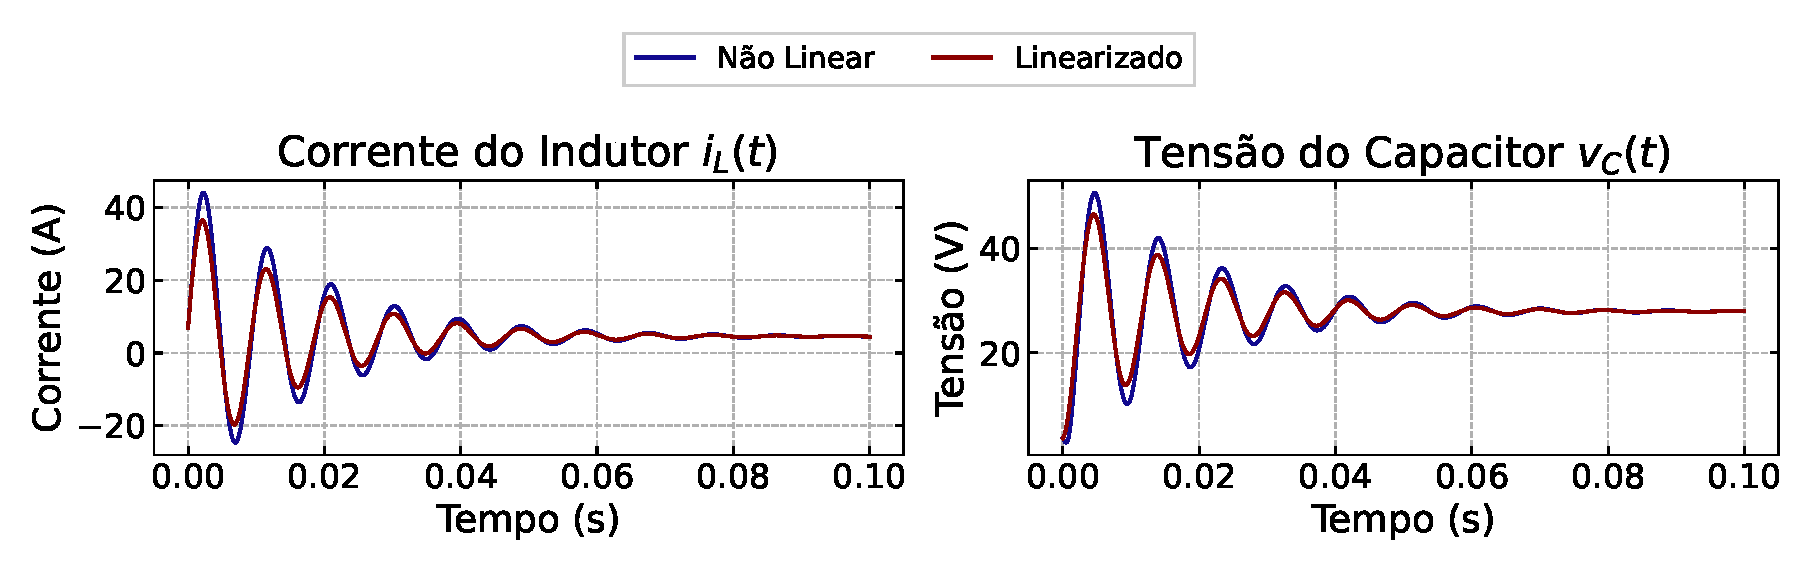
\includegraphics[width=1.\textwidth]{figuras/static-etm/buck/sim1/op1/result.eps}
    \caption{Estados do conversor.}
    \label{fig:buck_converter_constant_pcpl_static_etm_op1_duty_a}
  \end{subfigure}
  \\[6pt]
  \begin{subfigure}{1.\textwidth}
    \centering
    \includegraphics[width=1.\textwidth]{figuras/static-etm/buck/sim1/op1/duty-cycle.eps}
    \caption{Duty Cycle $d(t)$}
    \label{fig:buck_converter_constant_pcpl_static_etm_op1_duty_b}
  \end{subfigure}
  \\[6pt]
  \begin{subfigure}{1.\textwidth}
    \centering
    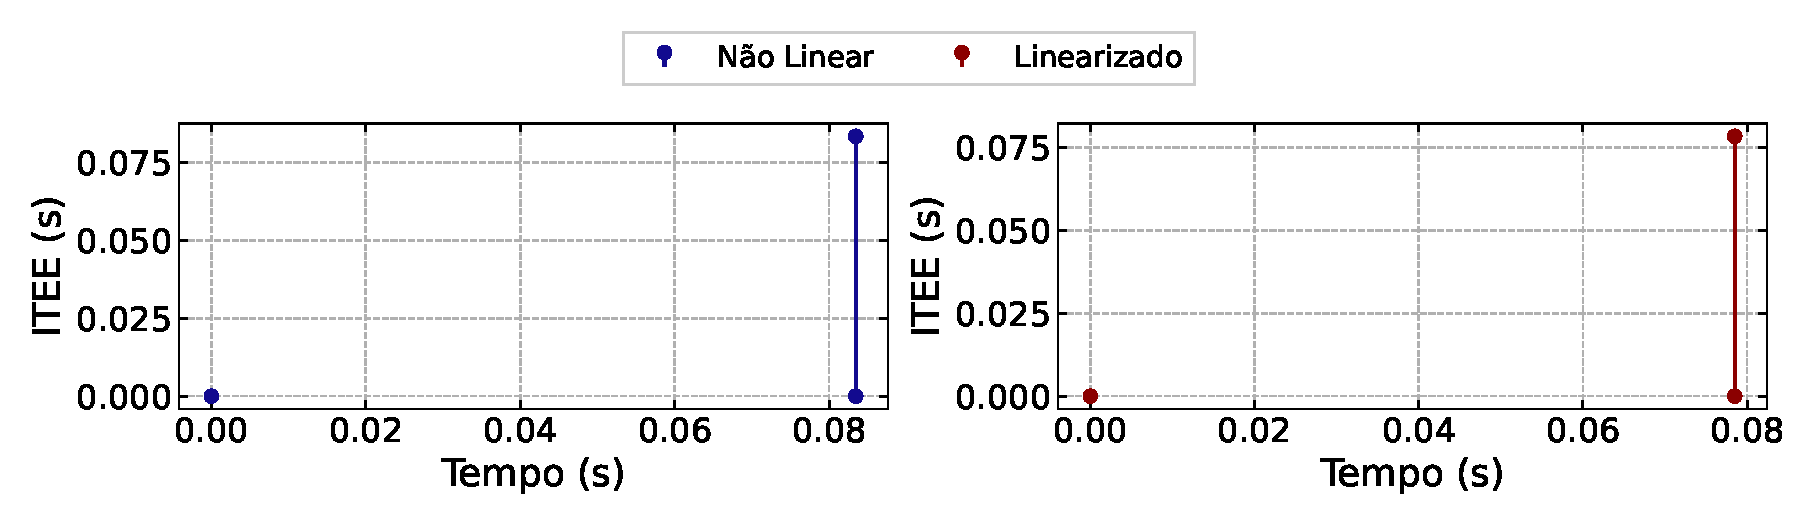
\includegraphics[width=1.\textwidth]{figuras/static-etm/buck/sim1/op1/inter-event-times.eps}
    \caption{Intervalo de tempo entre eventos.}
    \label{fig:buck_converter_constant_pcpl_static_etm_op1_duty_c}
  \end{subfigure}
  \caption{Estados $i_L(t)$ e $v_C(t)$, a entrada duty cycle $d(t)$ e os \acrshortpl{itee} do conversor Buck em torno do ponto $P_{\mathrm{o}, 1}$ sob sinal de pertubação $P_{\mathrm{cpl}}(t)$ constante e \acrshort{etm} estático.}
\end{figure}

Na \autoref{fig:buck_converter_constant_pcpl_static_etm_op1_duty_a}, é apresentada a evolução da entrada do sistema $d(t)$ durante toda a simulação. Durante a simulação do conversor em torno do ponto $P_{\mathrm{o}, 1}$, a entrada permanece constante até 0,08 s, momento em que ocorre um aumento. Este comportamento indica que entre 0 e 0,08 segundos, nenhum novo evento foi acionado para atualizar o controlador com novos estados, ou seja, a condição da lei de acionamento não era atendida e, portanto, o controlador tinha acesso apenas ao último estado transmitido mantido pelo \acrshort{zoh}. Quando atingiu o tempo de 0,08 s, a condição da lei de acionamento do \acrshort{etm} estático foi satisfeita, resultando no acionamento de um novo evento e permitindo a transmissão de um novo estado. Consequentemente, uma nova entrada é obtida e foi mantida até o final da simulação. Portanto, durante a simulação do conversor Buck em torno do ponto $P_{\mathrm{o}, 1}$, apenas dois eventos foram acionados, conforme pode ser confirmado pelo gráfico dos \acrshortpl{itee} na \autoref{fig:buck_converter_constant_pcpl_static_etm_op2_duty_b}.

\begin{figure}[H]
  \centering
  \captionsetup{justification=centering}
  \begin{subfigure}{1.\textwidth}
    \centering
    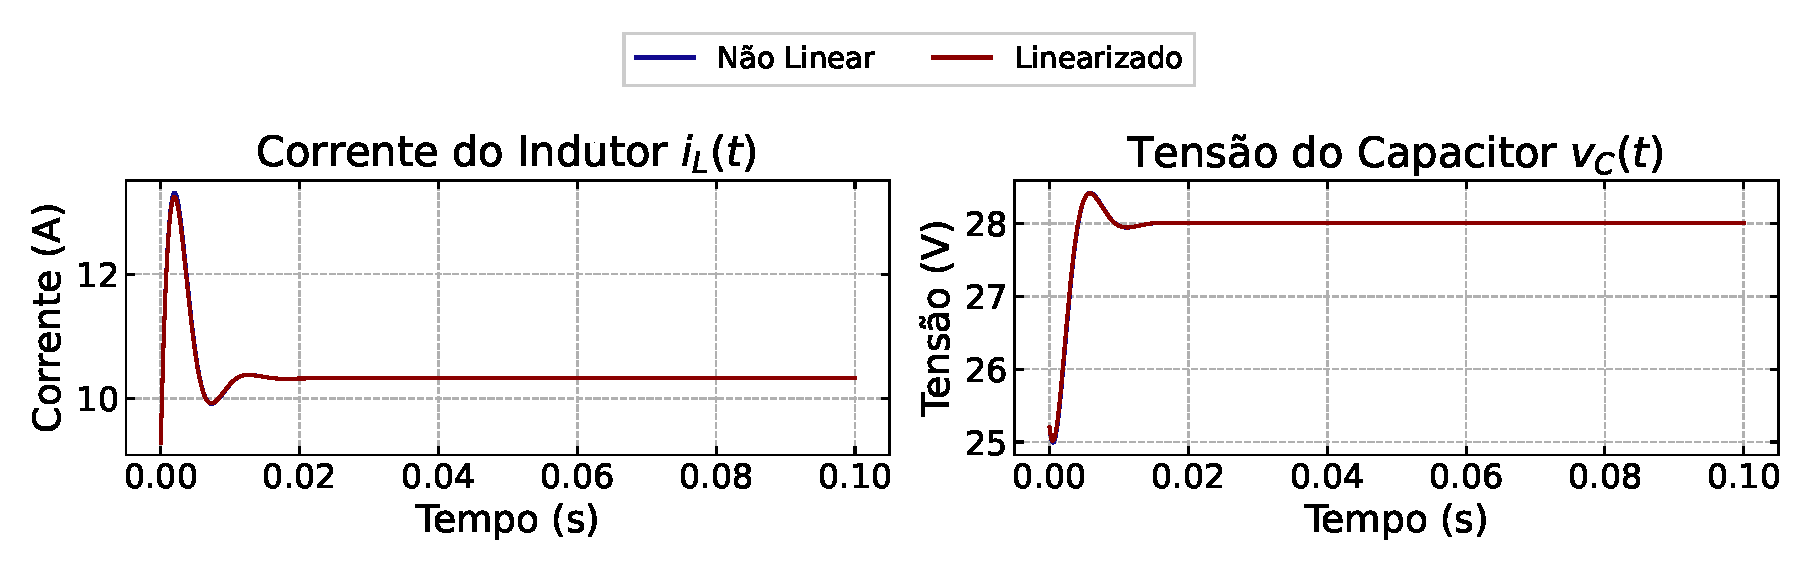
\includegraphics[width=1.\textwidth]{figuras/static-etm/buck/sim1/op2/result.eps}
    \caption{Estados do conversor.}
    \label{fig:buck_converter_constant_pcpl_static_etm_op2_duty_a}
  \end{subfigure}
  \\[6pt]
  \begin{subfigure}{1.\textwidth}
    \centering
    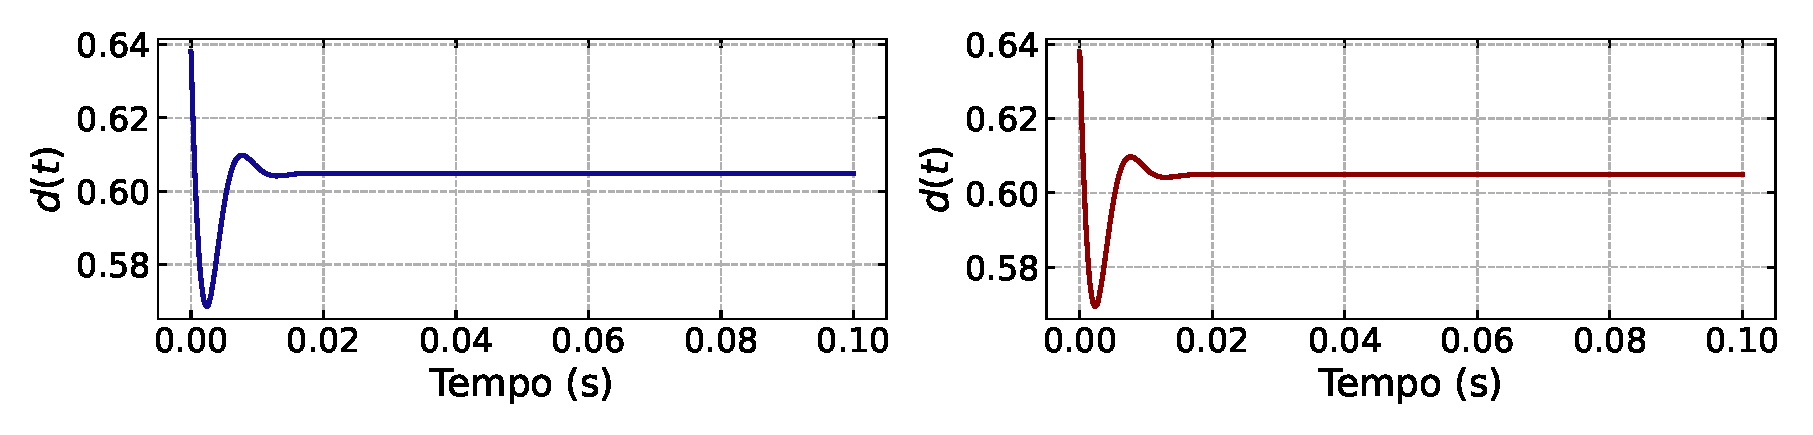
\includegraphics[width=1.\textwidth]{figuras/static-etm/buck/sim1/op2/duty-cycle.eps}
    \caption{Duty Cycle $d(t)$}
    \label{fig:buck_converter_constant_pcpl_static_etm_op2_duty_b}
  \end{subfigure}
  \\[6pt]
  \begin{subfigure}{1.\textwidth}
    \centering
    \includegraphics[width=1.\textwidth]{figuras/static-etm/buck/sim1/op2/inter-event-times.eps}
    \caption{Intervalo de tempo entre eventos.}
    \label{fig:buck_converter_constant_pcpl_static_etm_op2_duty_c}
  \end{subfigure}
  \caption{Estados $i_L(t)$ e $v_C(t)$, a entrada duty cycle $d(t)$ e os \acrshortpl{itee} do conversor Buck em torno do ponto $P_{\mathrm{o}, 2}$ sob sinal de pertubação $P_{\mathrm{cpl}}(t)$ constante e \acrshort{etm} estático.}
\end{figure}

Por outro lado, durante a simulação do conversor Buck em torno do ponto $P_{\mathrm{o}, 2}$, observou-se que o \acrshort{etm} desencadeou uma série de novos eventos, como mostrado na \autoref{fig:buck_converter_constant_pcpl_static_etm_op2_duty_b}. Esse padrão de comportamento era previsto devido à instabilidade associada ao ponto $P_{\mathrm{o}, 2}$. À medida que o sistema tende a se desviar gradualmente nesse ponto, o erro de transmissão aumenta, resultando na função de acionamento $\Gamma$ do \acrshort{etm} tornando-se negativa, o que permite o disparo de novos eventos de transmissão. Esse ciclo pode se repetir várias vezes ao longo do tempo, mesmo que o sistema, em malha fechada, eventualmente se estabilize. Portanto, é esperado que o \acrshort{etm} continue a realizar acionamentos mesmo após a estabilização do sistema.

\begin{figure}[H]
  \centering
  \captionsetup{justification=centering}
  \begin{subfigure}{1.\textwidth}
    \centering
    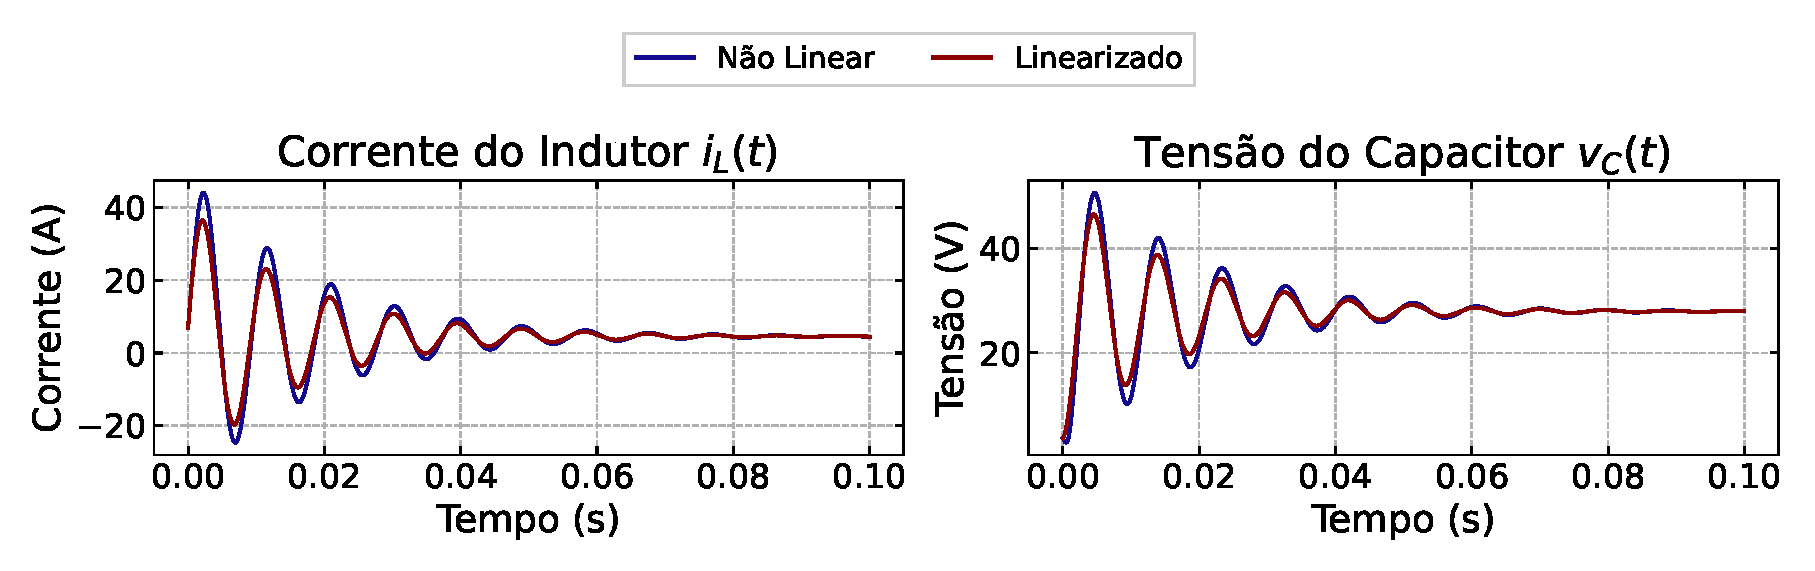
\includegraphics[width=1.\textwidth]{figuras/dynamic-etm/buck/sim1/op1/result.eps}
    \caption{Estados do conversor.}
    \label{fig:buck_converter_constant_pcpl_dynamic_etm_op1_a}
  \end{subfigure}
  \\[6pt]
  \begin{subfigure}{1.\textwidth}
    \centering
    \includegraphics[width=1.\textwidth]{figuras/dynamic-etm/buck/sim1/op1/duty-cycle.eps}
    \caption{Duty Cycle $d(t)$}
    \label{fig:buck_converter_constant_pcpl_dynamic_etm_op1_b}
  \end{subfigure}
  \\[6pt]
  \begin{subfigure}{1.\textwidth}
    \centering
    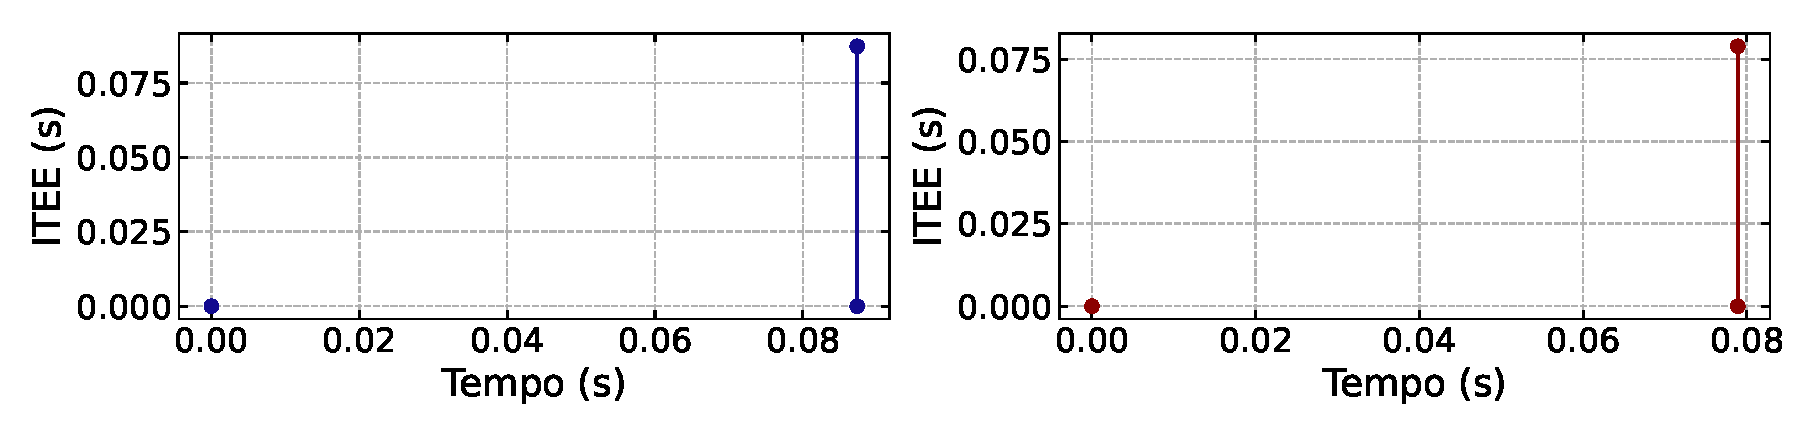
\includegraphics[width=1.\textwidth]{figuras/dynamic-etm/buck/sim1/op1/inter-event-times.eps}
    \caption{Intervalo de tempo entre eventos.}
    \label{fig:buck_converter_constant_pcpl_dynamic_etm_op1_c}
  \end{subfigure}
  \caption{Estados $i_L(t)$, $v_C(t)$ e $\eta(t)$, a entrada duty cycle $d(t)$ e os \acrshortpl{itee} do conversor Buck em torno do ponto $P_{\mathrm{o}, 1}$ sob sinal de pertubação $P_{\mathrm{cpl}}(t)$ constante e \acrshort{etm} estático.}
  \label{fig:buck_converter_constant_pcpl_dynamic_etm_op1}
\end{figure}

\begin{figure}[H]
  \centering
  \captionsetup{justification=centering}
  \begin{subfigure}{1.\textwidth}
    \centering
    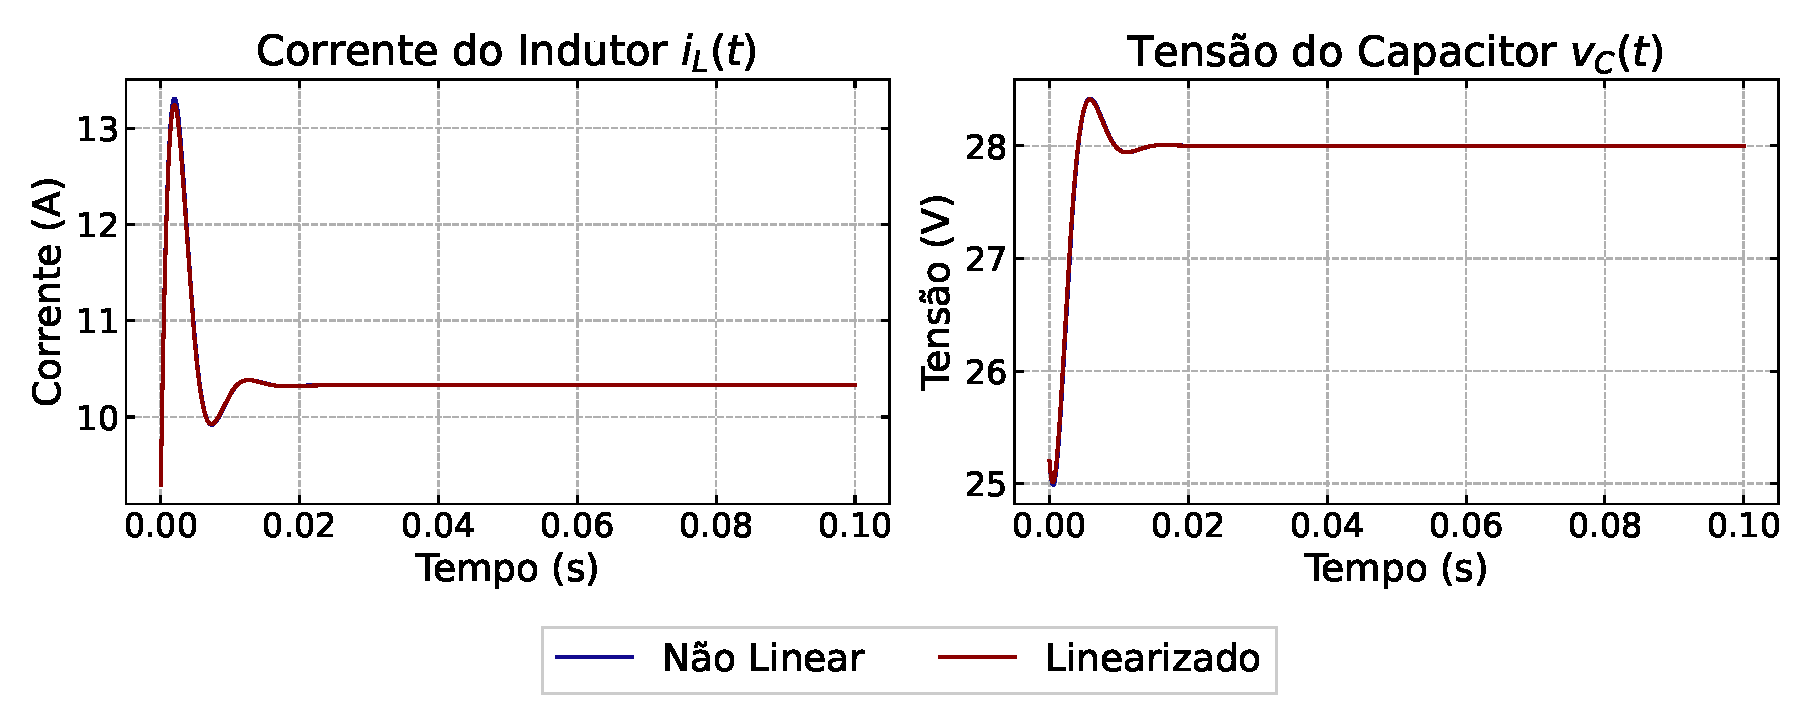
\includegraphics[width=1.\textwidth]{figuras/dynamic-etm/buck/sim1/op2/result.eps}
    \caption{Estados do conversor.}
    \label{fig:buck_converter_constant_pcpl_dynamic_etm_op2_a}
  \end{subfigure}
  \\[6pt]
  \begin{subfigure}{1.\textwidth}
    \centering
    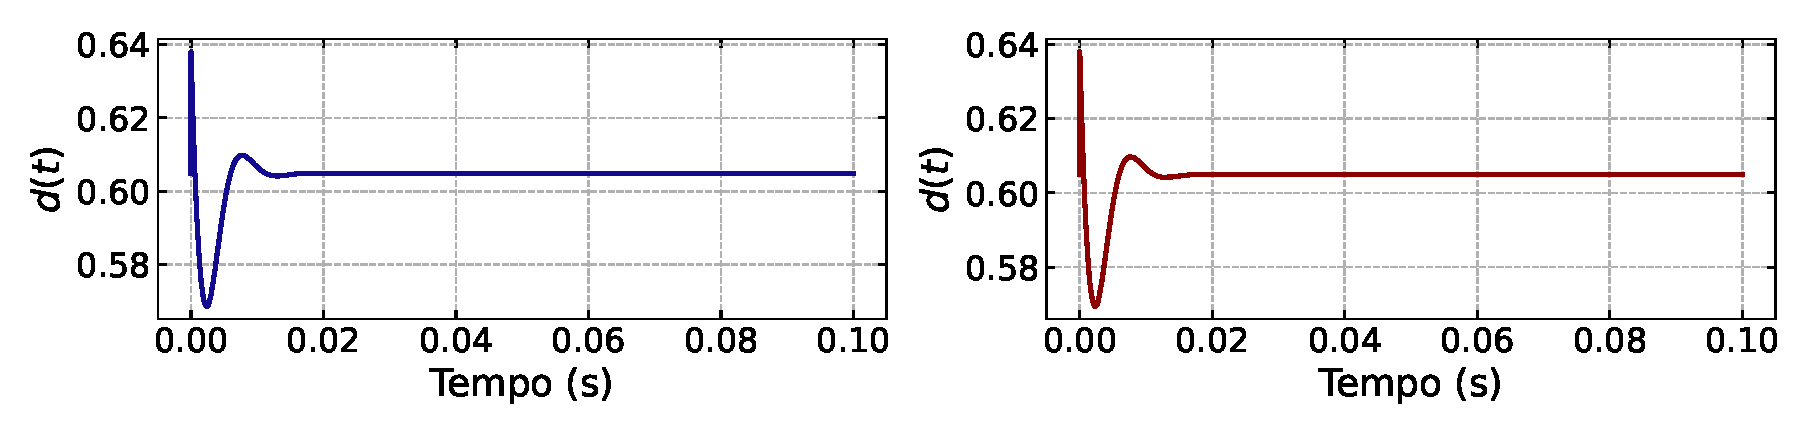
\includegraphics[width=1.\textwidth]{figuras/dynamic-etm/buck/sim1/op2/duty-cycle.eps}
    \caption{Duty Cycle $d(t)$}
    \label{fig:buck_converter_constant_pcpl_dynamic_etm_op2_b}
  \end{subfigure}
  \\[6pt]
  \begin{subfigure}{1.\textwidth}
    \centering
    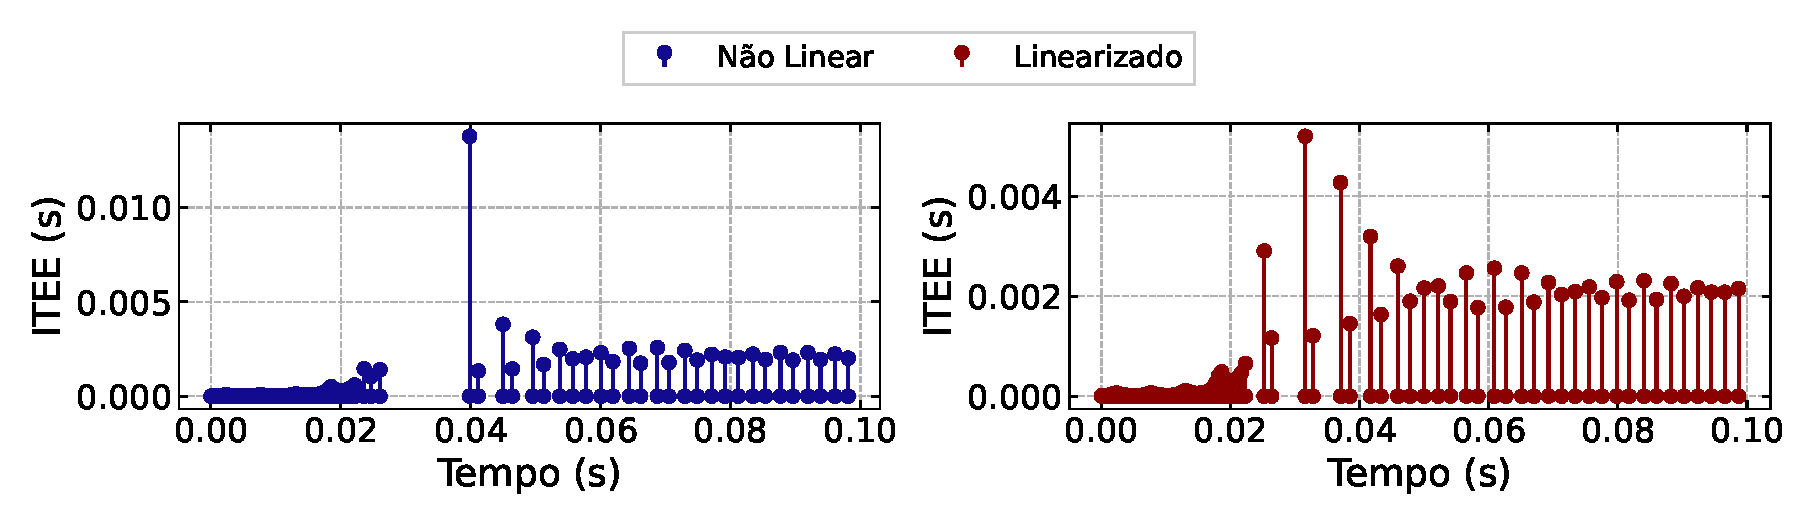
\includegraphics[width=1.\textwidth]{figuras/dynamic-etm/buck/sim1/op2/inter-event-times.eps}
    \caption{Intervalo de tempo entre eventos.}
    \label{fig:buck_converter_constant_pcpl_dynamic_etm_op2_c}
  \end{subfigure}
  \caption{Estados $i_L(t)$, $v_C(t)$ e $\eta(t)$, a entrada duty cycle $d(t)$ e os \acrshortpl{itee} do conversor Buck em torno do ponto $P_{\mathrm{o}, 2}$ no Cenário 1 e \acrshort{etm} estático.}
  \label{fig:buck_converter_constant_pcpl_dynamic_etm_op2}
\end{figure}

Em relação ao \acrshort{etm} dinâmico, durante a simulação foi obtido um comportamento semelhante ao estático em torno do ponto $P_{\mathrm{o}, 1}$, conforme ilustrado pelas Figuras \ref{fig:buck_converter_constant_pcpl_dynamic_etm_op1_a}, \ref{fig:buck_converter_constant_pcpl_dynamic_etm_op1_b} e \ref{fig:buck_converter_constant_pcpl_dynamic_etm_op1_c}. Não foram observadas diferenças significativas nesses casos. No entanto, ao analisar o ponto instável $P_{\mathrm{o}, 2}$ (Figura \ref{fig:buck_converter_constant_pcpl_dynamic_etm_op2}), destacamos uma vantagem do \acrshort{etm} dinâmico. Houve uma redução significativa na ocorrência de eventos perturbadores, especialmente notável após 0,4 segundos. Os intervalos entre esses eventos aumentam para aproximadamente 2 milissegundos, contrastando com os 60 microssegundos observados com o \acrshort{etm} estático. Esses resultados sugerem uma eficácia adicional do \acrshort{etm} dinâmico em pontos de operação instável, promovendo uma maior estabilidade e robustez ao sistema.

\begin{figure}[H]
  \centering
  \captionsetup{justification=centering}
  \begin{subfigure}{1.\textwidth}
    \centering
    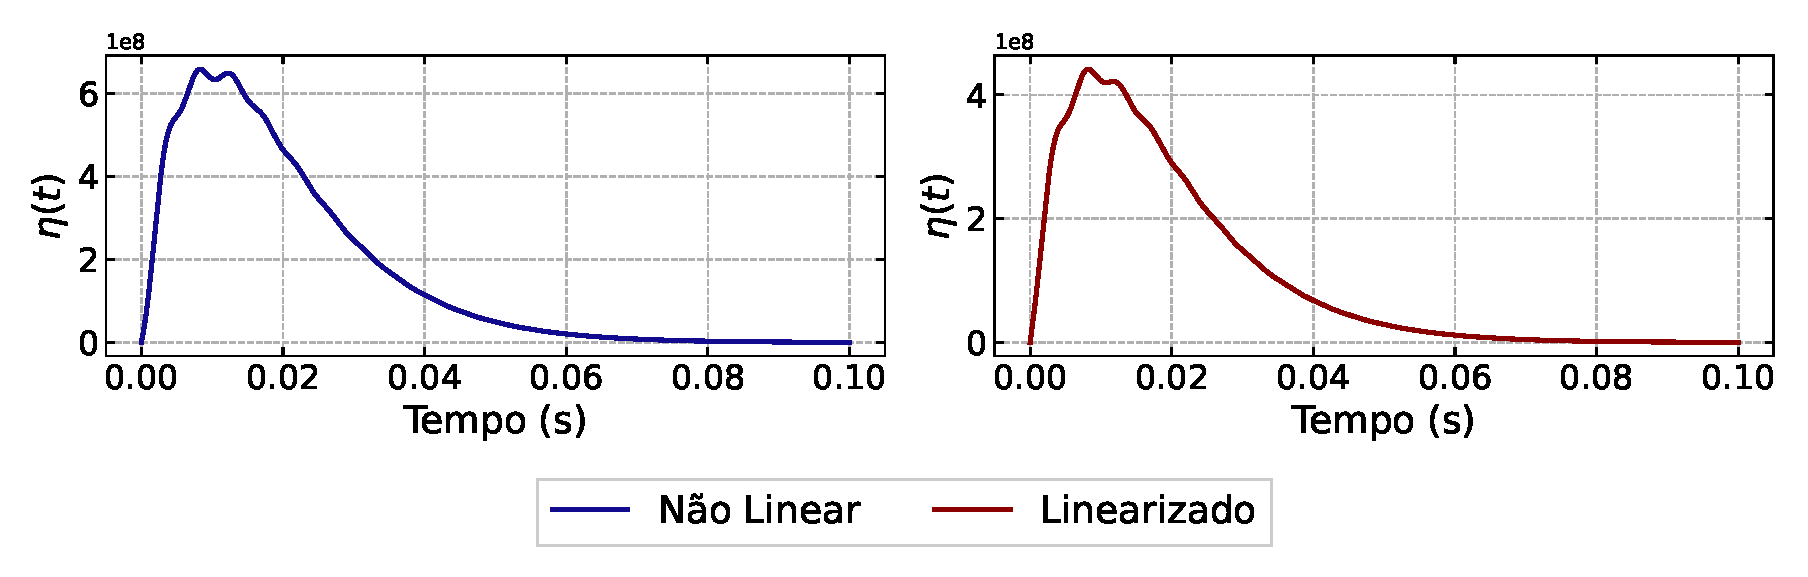
\includegraphics[width=1.\textwidth]{figuras/dynamic-etm/buck/sim1/op1/eta.eps}
    \caption{Ponto de operação $P_{\mathrm{o}, 1}$}
    % \label{fig:buck_converter_dynamic_pcpl_dynamic_etm_op1_d}
  \end{subfigure}
  \\[6pt]
  \begin{subfigure}{1.\textwidth}
    \centering
    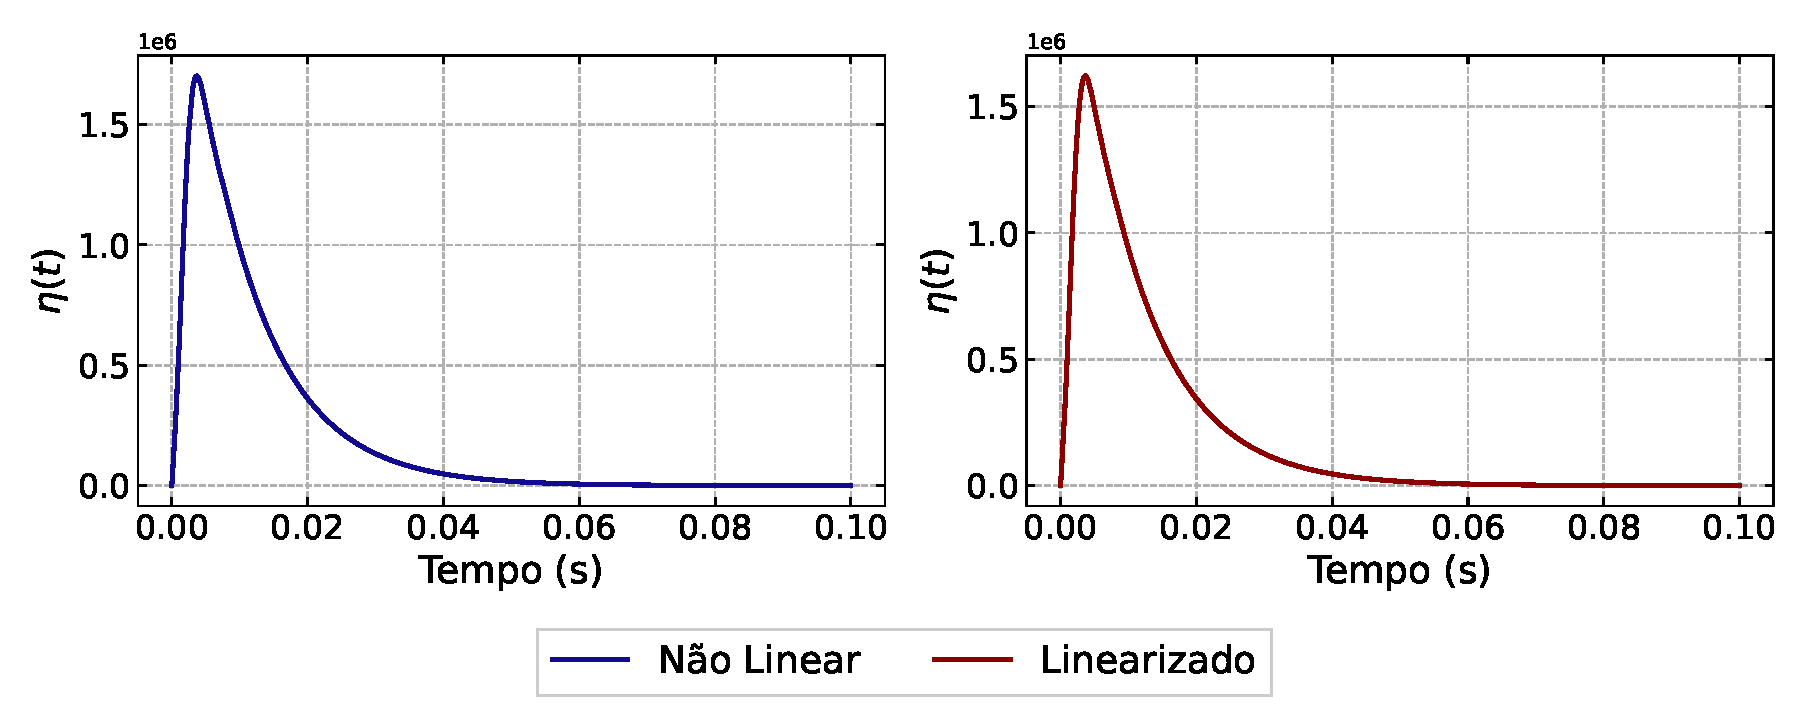
\includegraphics[width=1.\textwidth]{figuras/dynamic-etm/buck/sim1/op2/eta.eps}
    \caption{Ponto de operação $P_{\mathrm{o}, 2}$}
    \label{fig:buck_converter_dynamic_pcpl_dynamic_etm_op2_d}
  \end{subfigure}
  \caption{Variável dinâmica $\eta(t)$ do \acrshort{etm} dinâmico sob sinal de pertubação $P_{\mathrm{cpl}}(t)$ constante.}
  \label{fig:buck_converter_constant_pcpl_dynamic_etm_eta}
\end{figure}

Na \autoref{fig:buck_converter_constant_pcpl_dynamic_etm_eta}, são apresentadas as evoluções temporais da variável dinâmica $\eta(n)$ durante a simulação do conversor Buck nos \acrshortpl{po} estável e instável. É possível observar que $\eta(t)$ é não negativa para todos os valores de $t$, conforme esperado, e converge para o equilíbrio na origem ($\eta = 0$). O efeito de $\eta(t)$ produz o aumento dos \acrshort{itee}, como pode-se observar ao comparar as Figuras \ref{fig:buck_converter_constant_pcpl_dynamic_etm_op1_c} e \ref{fig:buck_converter_constant_pcpl_dynamic_etm_op2_c}, pois se comporta como um buffer que armazena a redução desnecessária da função de Lyapunov $V(x)$.

% Esta análise investiga a relação entre o parâmetro $\mu$ do problema multiobjetivo e o comportamento do sistema em malha fechada. Para isso, o conversor Buck é considerado operando no ponto de operação instável $P_{\mathrm{o}, 2}$  com um sinal de perturbação constante igual ao valor do ponto de operação. O parâmetro $\mu$ variou entre 0 e 1, e foram obtidos o tempo de acomodação de 2\% e o tempo médio dos intervalos de tempo entre eventos.

A \autoref{fig:buck_converter_rho} apresenta os resultados obtidos ao variar o parâmetro $\rho$ da função objetivo do problema de otimização \eqref{eq:optimization_problem}. À medida que $\rho$ aumenta, nota-se uma diminuição gradual na média dos \acrshortpl{itee}, aproximando-se de zero, enquanto os tempos de acomodação aumentam. Os tempos de acomodação entre o \acrshort{etm} dinâmico e estático mostraram-se notavelmente semelhantes, assim como entre os modelos não linear e linearizado. No entanto, é possível observar que as médias dos \acrshortpl{itee} são maiores no \acrshort{etm} dinâmico em comparação com o \acrshort{etm} estático.

\begin{figure}[H]
  \centering
  \captionsetup{justification=centering}
  \begin{subfigure}{1.\textwidth}
    \centering
    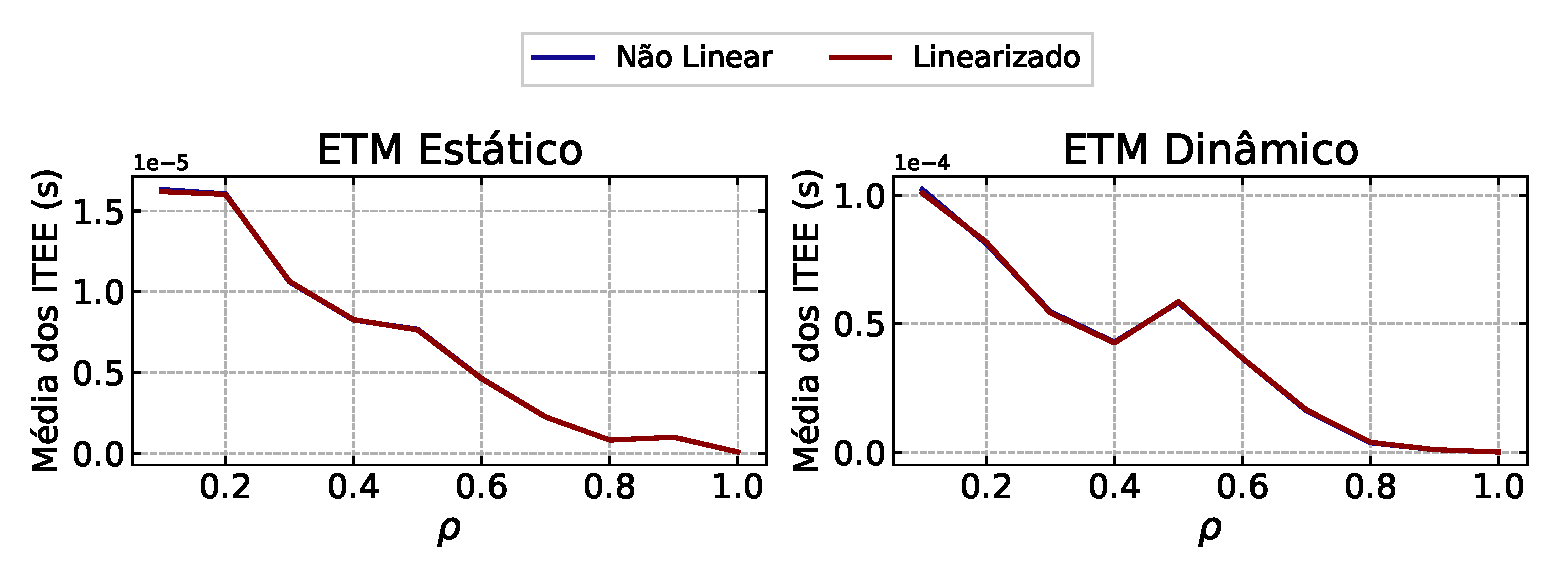
\includegraphics[width=1.\textwidth]{figuras/buck/itee-mean.eps}
    \caption{Médias dos \acrshortpl{itee} em relação a variação de $\rho$}
  \end{subfigure}
  \\[6pt]
  \begin{subfigure}{1.\textwidth} 
    \centering
    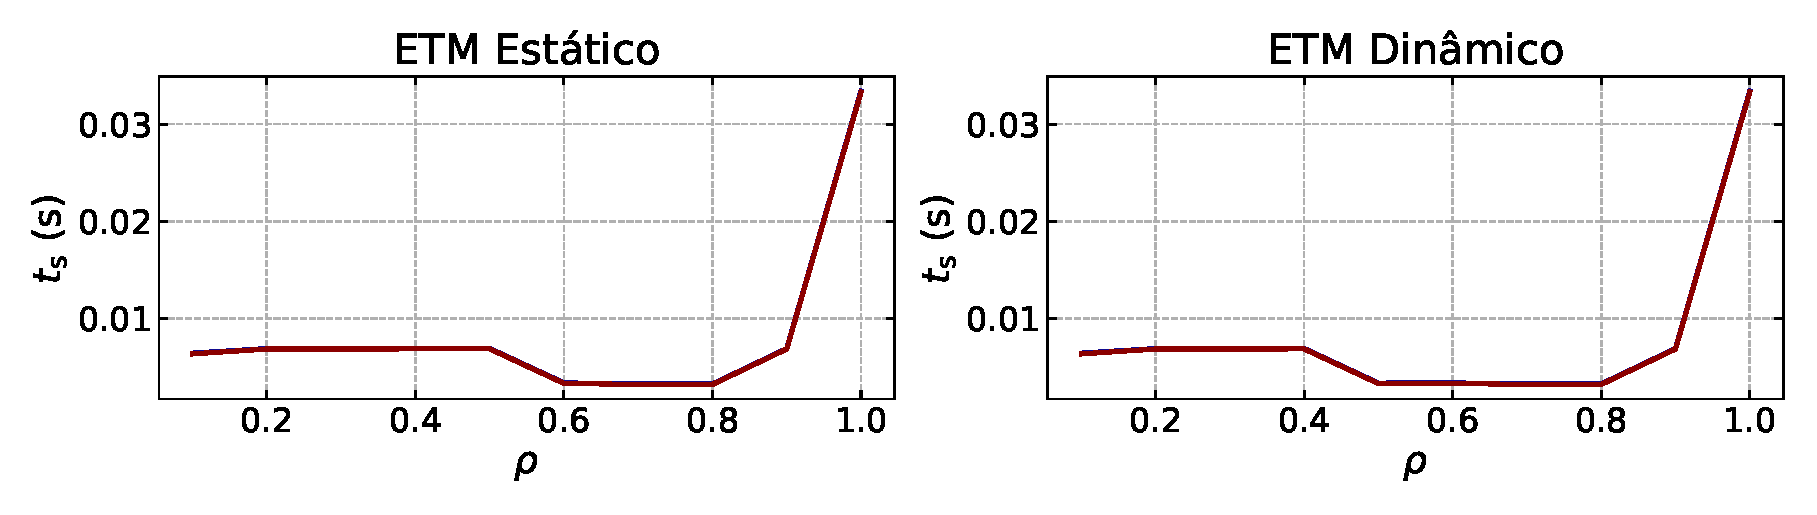
\includegraphics[width=1.\textwidth]{figuras/buck/ts.eps}
    \caption{Os tempos de acomodação dos estados do sistema sob o \acrshort{etm} estático e dinâmico em resposta às mudanças em $\rho$.}
  \end{subfigure}
  \caption{Resposta do conversor Buck sob variação do parâmetro $\rho$.}
  \label{fig:buck_converter_rho}
\end{figure}


As Figuras \ref{fig:classic_buck_cen1_op1} e \ref{fig:classic_buck_cen1_op2} apresentam o comportamento do conversor Buck neste cenário, sob um controlador desenvolvido com base no critério de estabilidade de Hurwitz. É possível observar que o desempenho do sistema é diferente do comportamento sob o ETC. Enquanto o conversor permanece instável em malha fechada ao redor do ponto instável, sua resposta em torno do ponto estável é notavelmente lenta.

\begin{figure}[H]
  \centering
  \captionsetup{justification=centering}
  \begin{subfigure}{1.\textwidth}
    \centering
    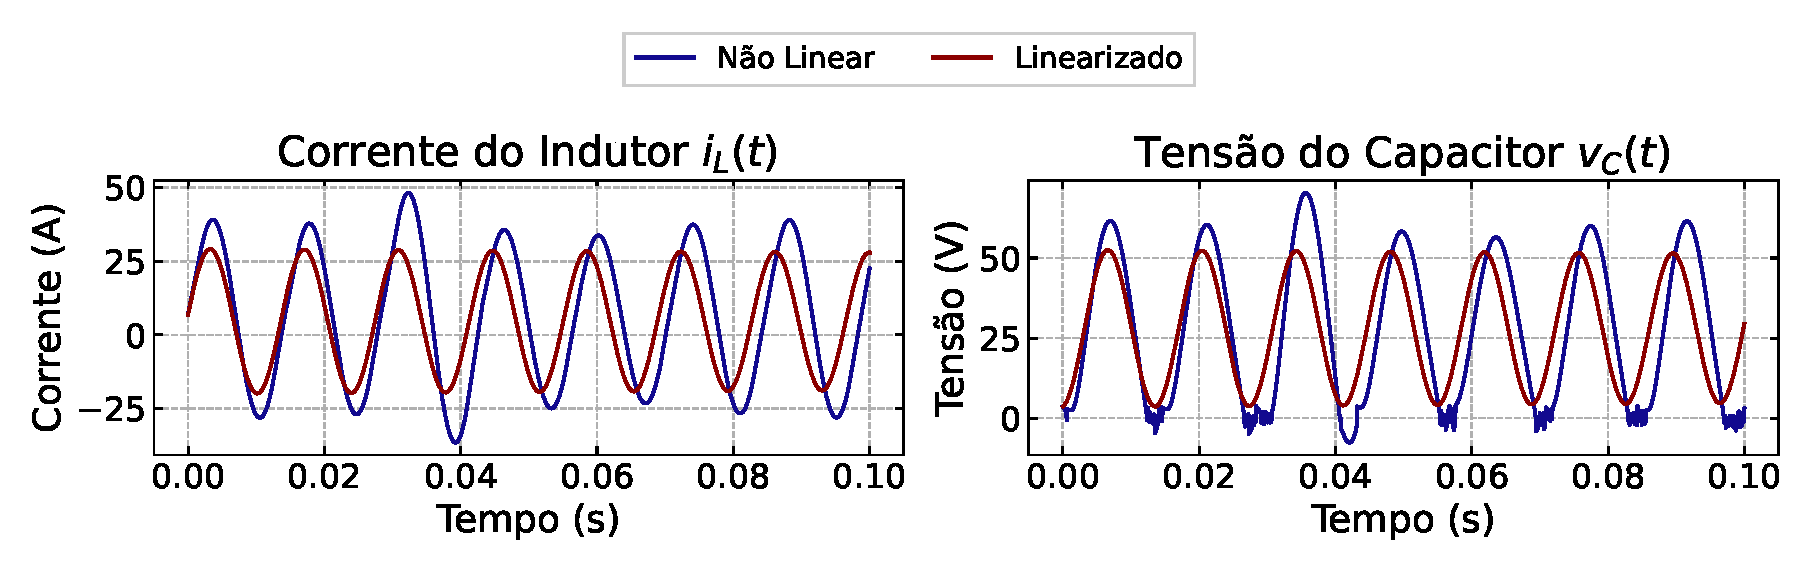
\includegraphics[width=1.\textwidth]{figuras/classic/buck/sim1/op1/result.eps}
    \caption{Estados do Sistema $i_L(t)$  e $v_C(t)$}
    % \label{fig:buck_converter_dynamic_pcpl_dynamic_etm_op1_d}
  \end{subfigure}
  \\[6pt]
  \begin{subfigure}{1.\textwidth}
    \centering
    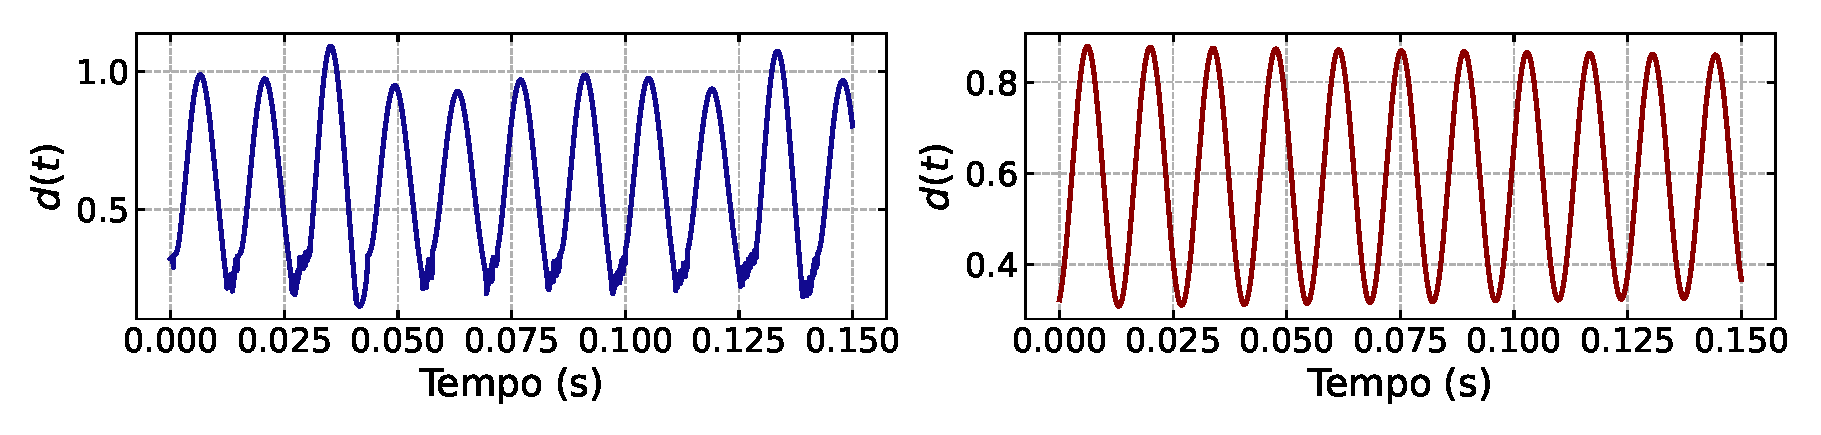
\includegraphics[width=1.\textwidth]{figuras/classic/buck/sim1/op1/duty-cycle.eps}
    \caption{Entrada controlável do Sistema $d(t)$}
  \end{subfigure}
  \caption{Conversor Buck no Cenário 1 operando em torno de $P_{\mathrm{o}, 1}$ sob controlador projetado utilizando o critério de estabilidade de Hurwitz.}
  \label{fig:classic_buck_cen1_op1}
  \begin{subfigure}{1.\textwidth}
    \centering
    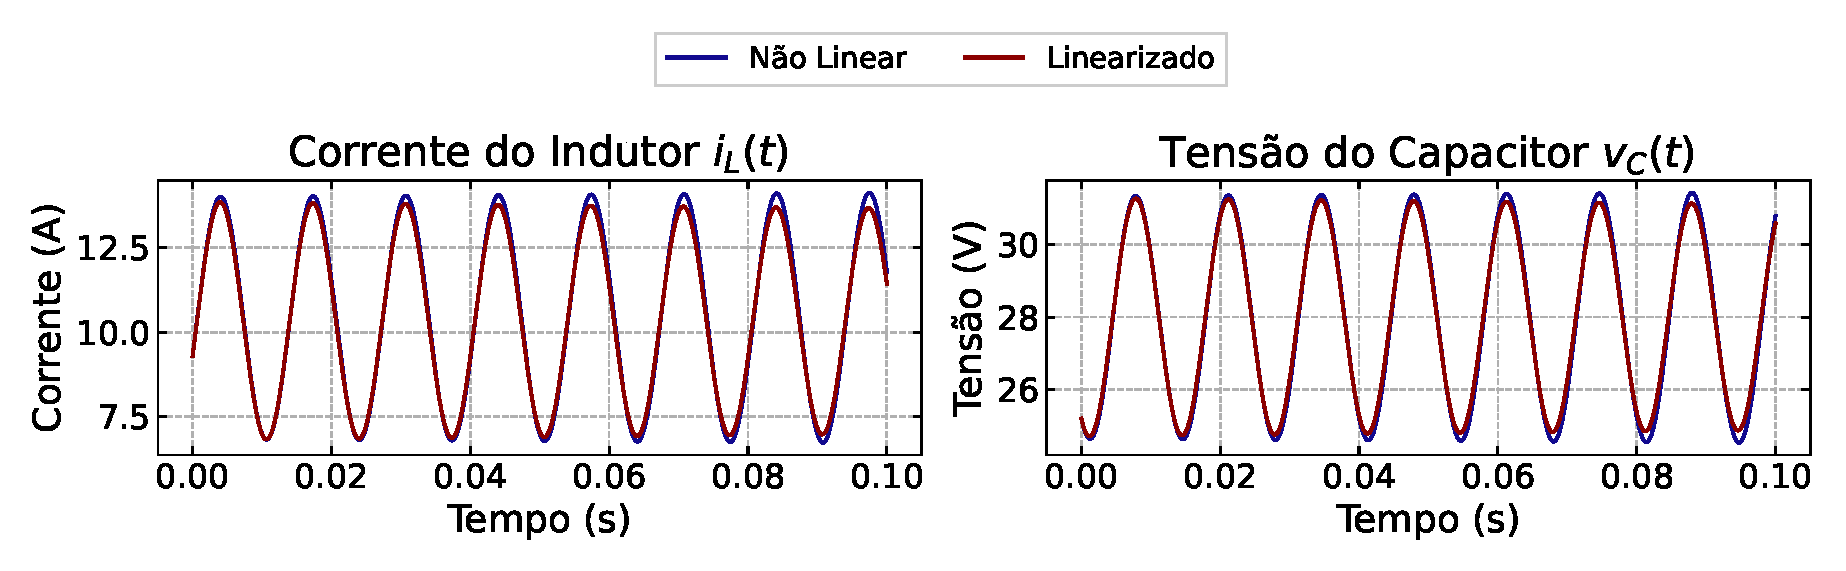
\includegraphics[width=1.\textwidth]{figuras/classic/buck/sim1/op2/result.eps}
    \caption{Estados do Sistema $i_L(t)$  e $v_C(t)$}
  \end{subfigure}
  \\[6pt]
  \begin{subfigure}{1.\textwidth}
    \centering
    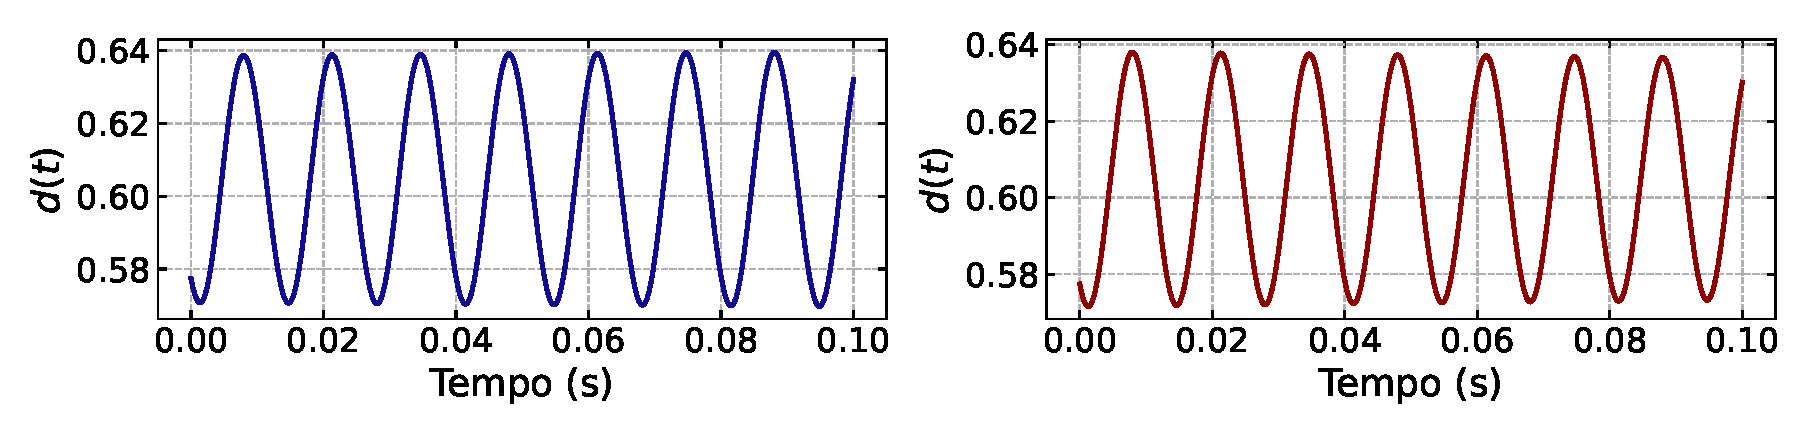
\includegraphics[width=1.\textwidth]{figuras/classic/buck/sim1/op2/duty-cycle.eps}
    \caption{Entrada controlável do Sistema $d(t)$}
  \end{subfigure}
  \caption{Conversor Buck no Cenário 1 em torno de $P_{\mathrm{o}, 2}$ sob controlador projetado utilizando o critério de estabilidade de Hurwitz.}
  \label{fig:classic_buck_cen1_op2}
\end{figure}

\subsubsection{Cenário 2}

Nesta simulação, o conversor Buck em malha fechada foi analisado sob a influência do sinal de perturbação variável. Na Figura \ref{fig:buck_converter_variable_pcpl_static_etm_op1_duty_a}, pode-se observar que o comportamento do conversor em torno do ponto $P_{\mathrm{o}, 1}$ em malha fechada é semelhante ao comportamento obtido em malha aberta. Além disso, foram necessários apenas três eventos de transmissão, como pode ser visto nas Figuras \ref{fig:buck_converter_variable_pcpl_static_etm_op1_duty_b} e \ref{fig:buck_converter_variable_pcpl_static_etm_op1_duty_c}.

\begin{figure}[H]
  \centering
  \captionsetup{justification=centering}
  \begin{subfigure}{1.\textwidth}
    \centering
    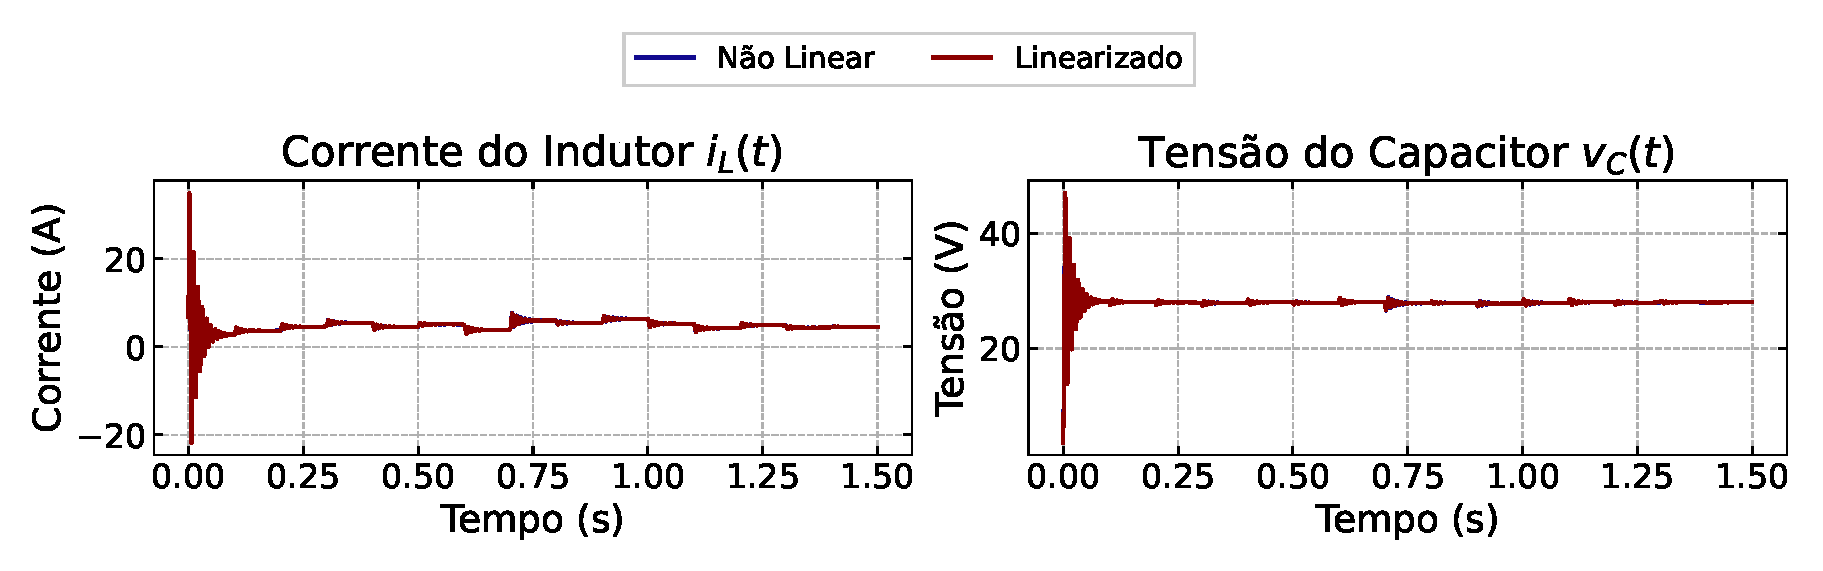
\includegraphics[width=1.\textwidth]{figuras/static-etm/buck/sim2/op1/result.eps}
    \caption{Estados do conversor.}
    \label{fig:buck_converter_variable_pcpl_static_etm_op1_duty_a}
  \end{subfigure}
  \\[6pt]
  \begin{subfigure}{1.\textwidth}
    \centering
    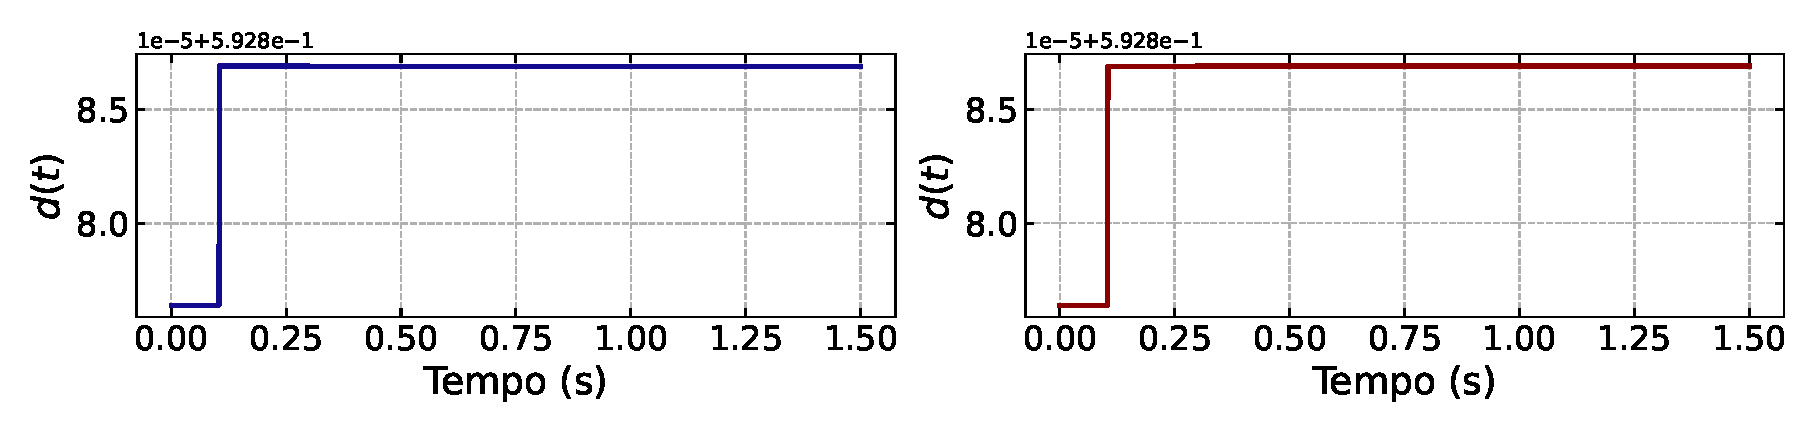
\includegraphics[width=1.\textwidth]{figuras/static-etm/buck/sim2/op1/duty-cycle.eps}
    \caption{Duty Cycle $d(t)$}
    \label{fig:buck_converter_variable_pcpl_static_etm_op1_duty_b}
  \end{subfigure}
  \\[6pt]
  \begin{subfigure}{1.\textwidth}
    \centering
    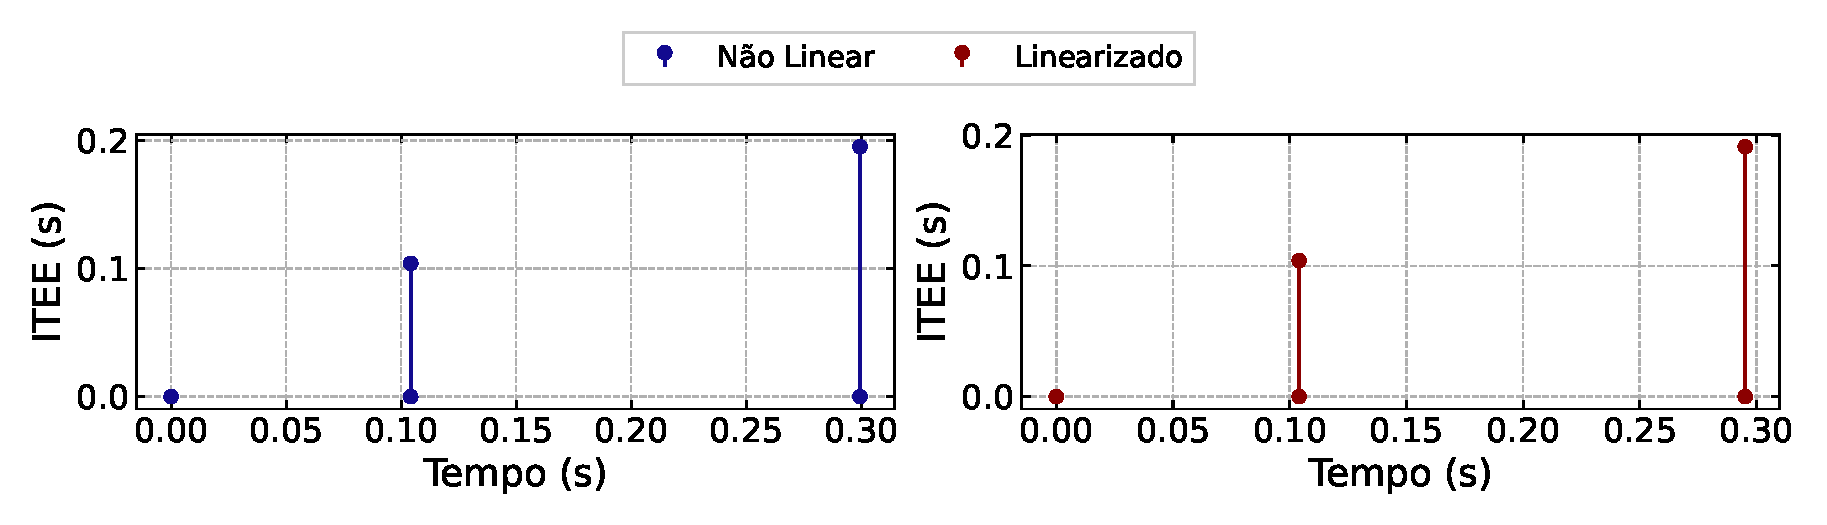
\includegraphics[width=1.\textwidth]{figuras/static-etm/buck/sim2/op1/inter-event-times.eps}
    \caption{Intervalo de tempo entre eventos.}
    \label{fig:buck_converter_variable_pcpl_static_etm_op1_duty_c}
  \end{subfigure}
  \caption{Estados $i_L(t)$ e $v_C(t)$, a entrada duty cycle $d(t)$ e os \acrshortpl{itee} do conversor Buck em torno do ponto $P_{\mathrm{o}, 1}$ sob sinal de pertubação $P_{\mathrm{cpl}}(t)$ variável e \acrshort{etm} estático.}
\end{figure}

Na simulação do conversor Buck em torno do ponto instável sob perturbação variável, o \acrshort{etm} estático assegurou a estabilidade do sistema durante toda a simulação (\autoref{fig:buck_converter_variable_pcpl_static_etm_op2_duty_a}). O aumento da magnitude da perturbação evidenciou a diferença entre os modelos não linear e linearizado. Após a estabilização, o \acrshort{etm} não necessitava acionar novos eventos, exceto em caso de alterações no sinal de perturbação (\autoref{fig:buck_converter_variable_pcpl_static_etm_op2_duty_c}). O sistema não linear apresentou menor demanda por eventos em comparação ao sistema linearizado e, ao final da simulação, o sistema se estabilizou no ponto de operação definido.

\begin{figure}[H]
  \centering
  \captionsetup{justification=centering}
  \begin{subfigure}{1.\textwidth}
    \centering
    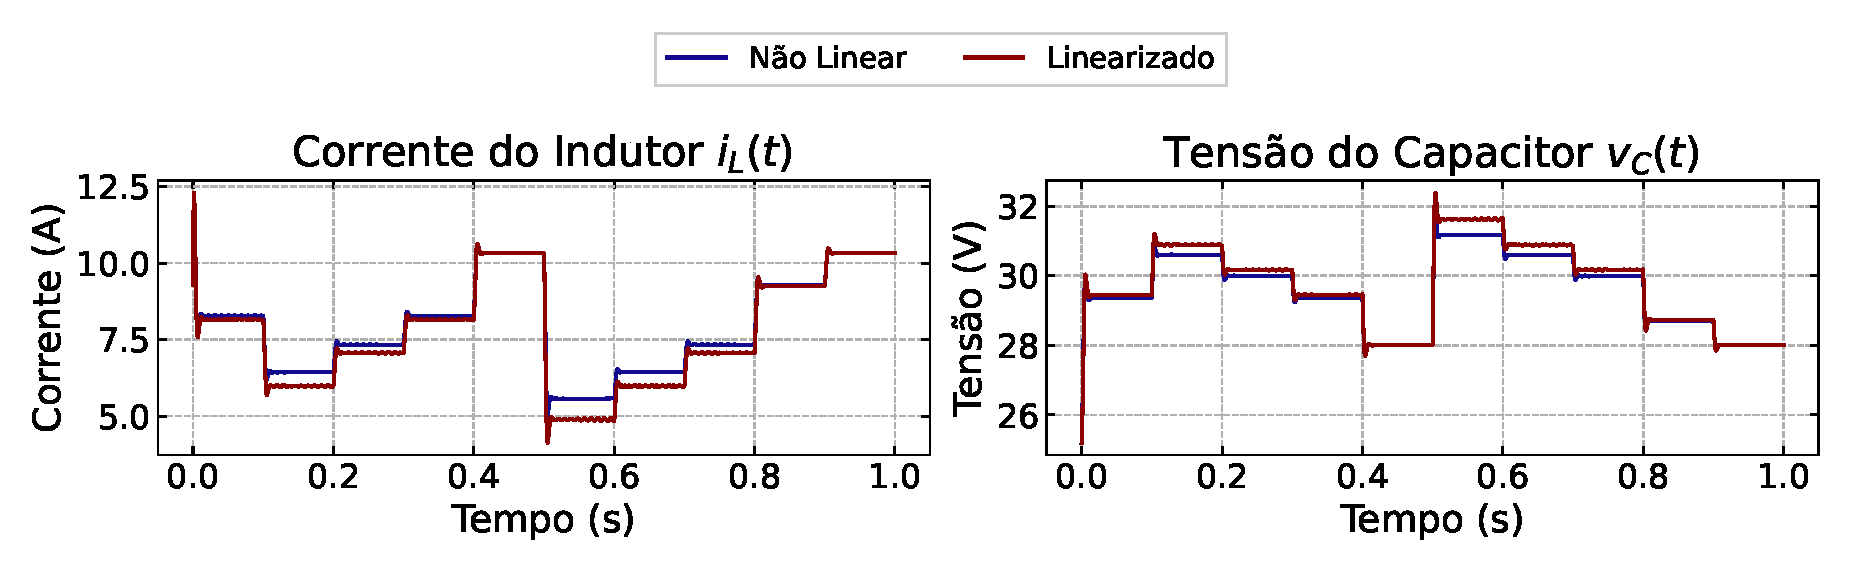
\includegraphics[width=1.\textwidth]{figuras/static-etm/buck/sim2/op2/result.eps}
    \caption{Estados do conversor.}
    \label{fig:buck_converter_variable_pcpl_static_etm_op2_duty_a}
  \end{subfigure}
  \\[6pt]
  \begin{subfigure}{1.\textwidth}
    \centering
    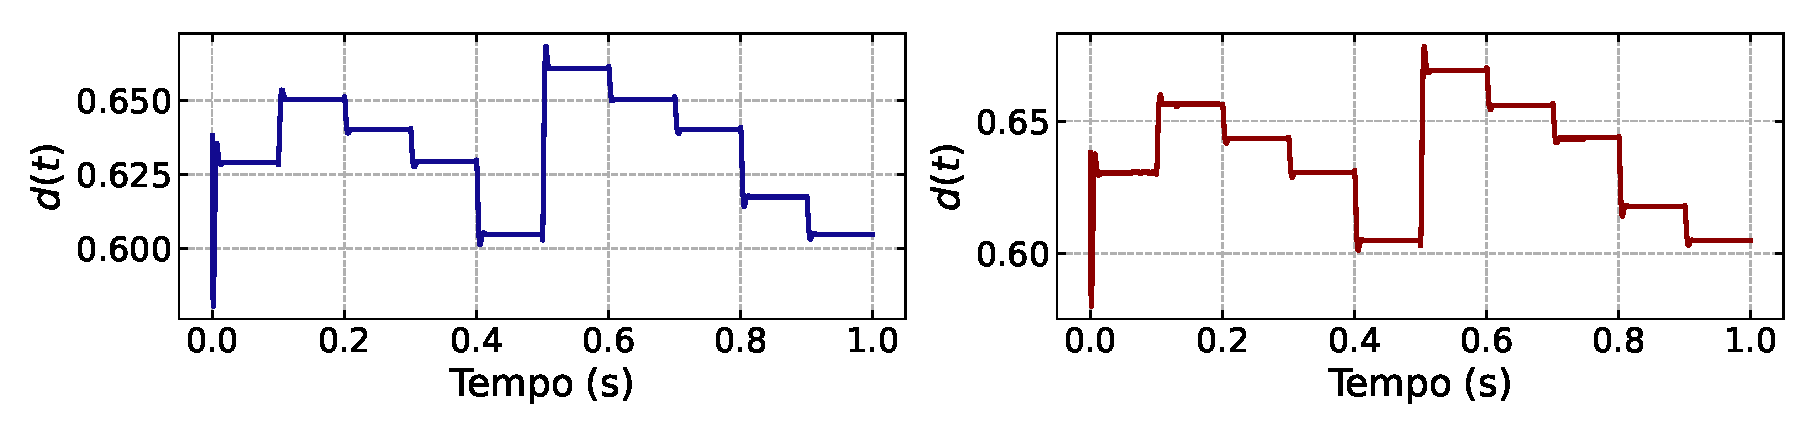
\includegraphics[width=1.\textwidth]{figuras/static-etm/buck/sim2/op2/duty-cycle.eps}
    \caption{Duty Cycle $d(t)$}
    \label{fig:buck_converter_variable_pcpl_static_etm_op2_duty_b}
  \end{subfigure}
  \\[6pt]
  \begin{subfigure}{1.\textwidth}
    \centering
    \includegraphics[width=1.\textwidth]{figuras/static-etm/buck/sim2/op2/inter-event-times.eps}
    \caption{Intervalo de tempo entre eventos.}
    \label{fig:buck_converter_variable_pcpl_static_etm_op2_duty_c}
  \end{subfigure}
  \caption{Estados $i_L(t)$ e $v_C(t)$, a entrada duty cycle $d(t)$ e os \acrshortpl{itee} do conversor Buck em torno do ponto $P_{\mathrm{o}, 2}$ sob sinal de pertubação $P_{\mathrm{cpl}}(t)$ variável e \acrshort{etm} estático.}
\end{figure}

No contexto do \acrshort{etm} dinâmico, ao analisar o comportamento do conversor Buck (Figura \ref{fig:buck_converter_variable_pcpl_dynamic_etm_op1}) em torno dos pontos estáveis, observamos uma semelhança com os resultados obtidos com o \acrshort{etm} estático. Tanto o modelo não linear quanto o linearizado exigem apenas alguns novos eventos, evidenciando uma estabilização da variável dinâmica do \acrshort{etm} na origem, conforme confirmado pela \autoref{fig:buck_converter_variable_pcpl_dynamic_etm_eta_a}.

\begin{figure}[H]
  \centering
  \captionsetup{justification=centering}
  \begin{subfigure}{1.\textwidth}
    \centering
    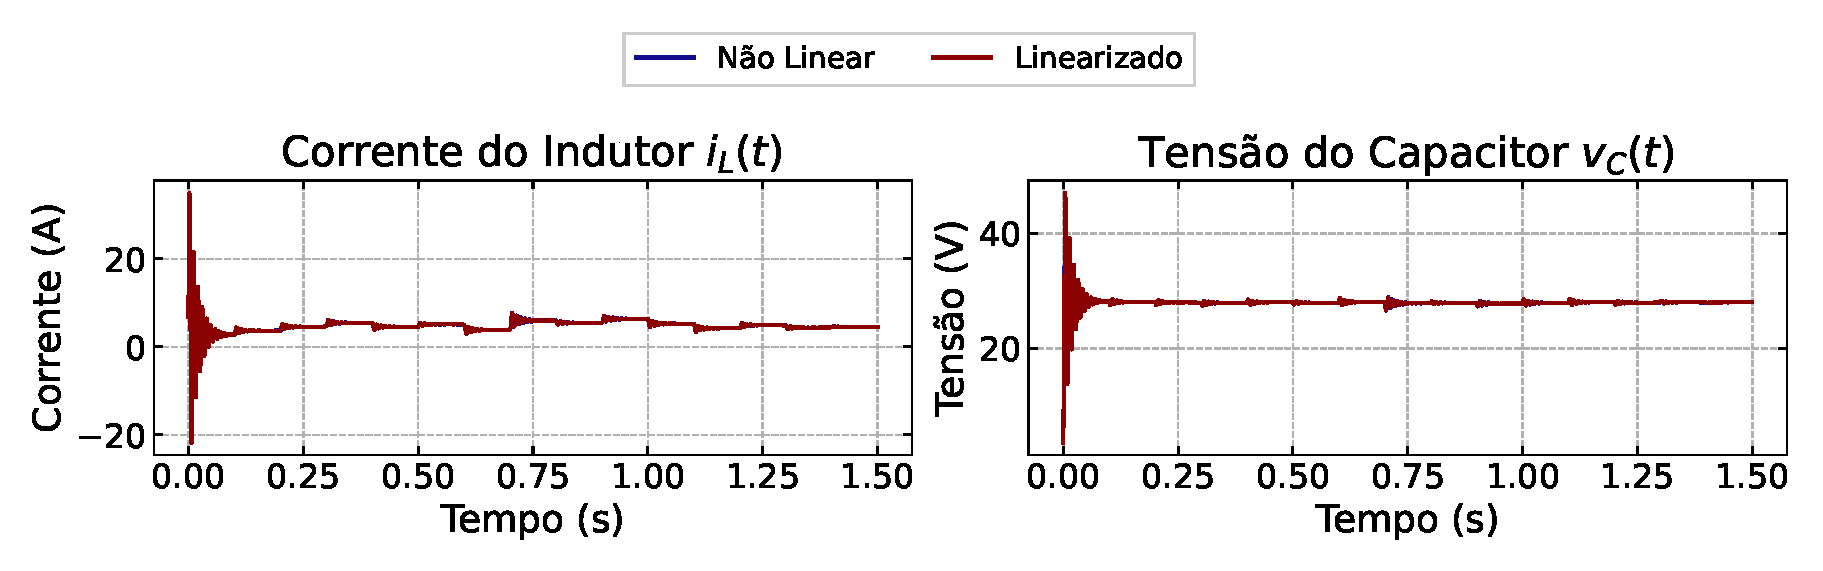
\includegraphics[width=1.\textwidth]{figuras/dynamic-etm/buck/sim2/op1/result.eps}
    \caption{Estados do conversor.}
    \label{fig:buck_converter_variable_pcpl_dynamic_etm_op1_a}
  \end{subfigure}
  \\[6pt]
  \begin{subfigure}{1.\textwidth}
    \centering
    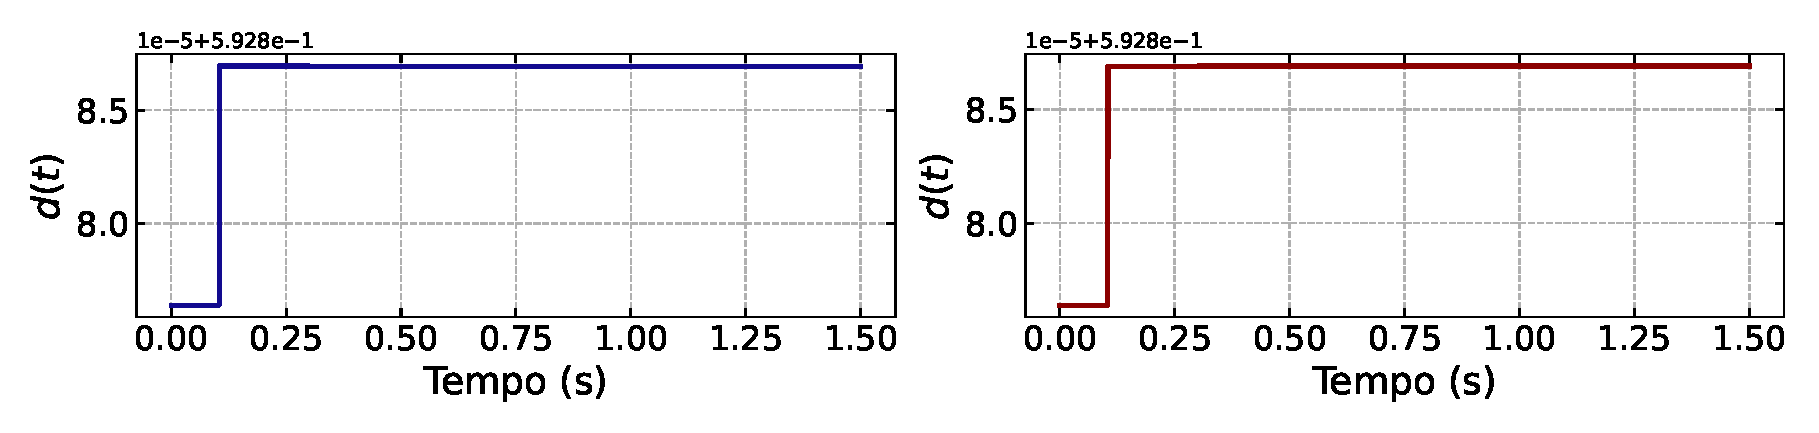
\includegraphics[width=1.\textwidth]{figuras/dynamic-etm/buck/sim2/op1/duty-cycle.eps}
    \caption{Duty Cycle $d(t)$}
    \label{fig:buck_converter_variable_pcpl_dynamic_etm_op1_b}
  \end{subfigure}
  \\[6pt]
  \begin{subfigure}{1.\textwidth}
    \centering
    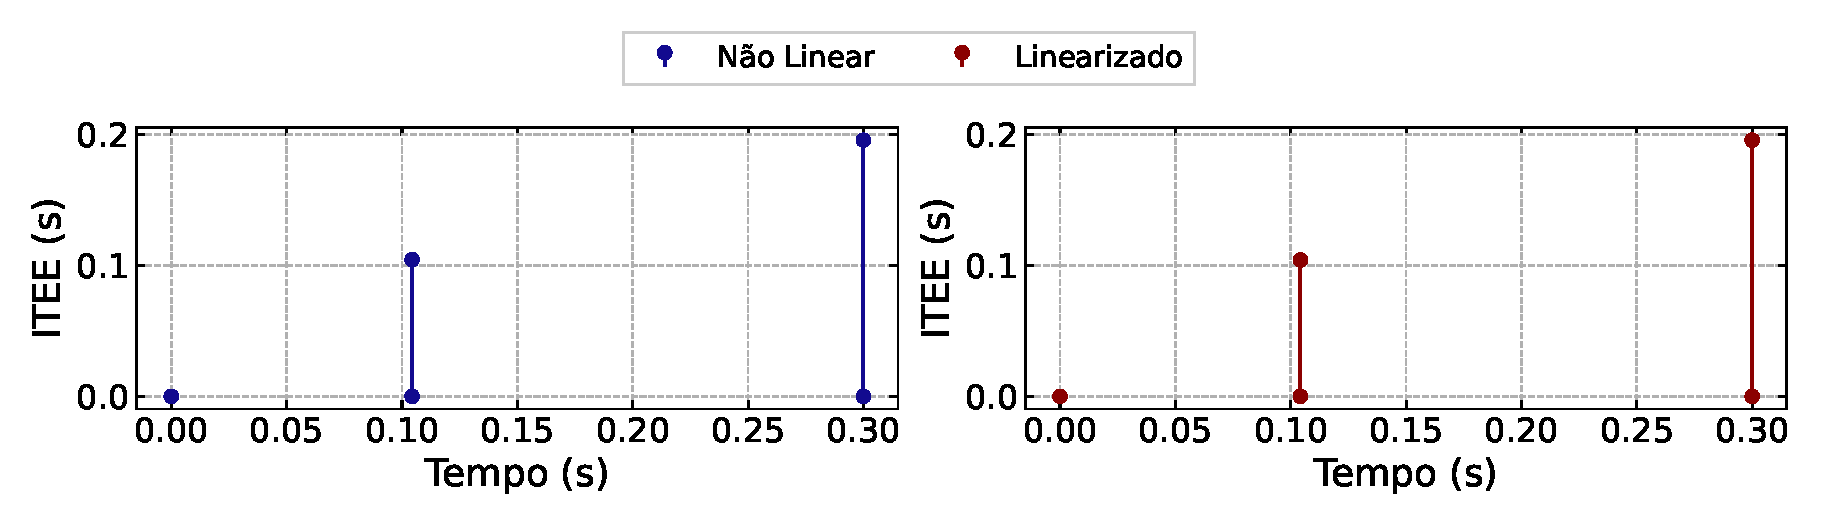
\includegraphics[width=1.\textwidth]{figuras/dynamic-etm/buck/sim2/op1/inter-event-times.eps}
    \caption{Intervalo de tempo entre eventos.}
    \label{fig:buck_converter_variable_pcpl_dynamic_etm_op1_c}
  \end{subfigure}
  \caption{Estados $i_L(t)$, $v_C(t)$ e $\eta(t)$, a entrada duty cycle $d(t)$ e os \acrshortpl{itee} do conversor Buck em torno do ponto $P_{\mathrm{o}, 1}$ sob sinal de pertubação $P_{\mathrm{cpl}}(t)$ variável e \acrshort{etm} estático.}
  \label{fig:buck_converter_variable_pcpl_dynamic_etm_op1}
\end{figure}

\begin{figure}[H]
  \centering
  \captionsetup{justification=centering}
  \begin{subfigure}{1.\textwidth}
    \centering
    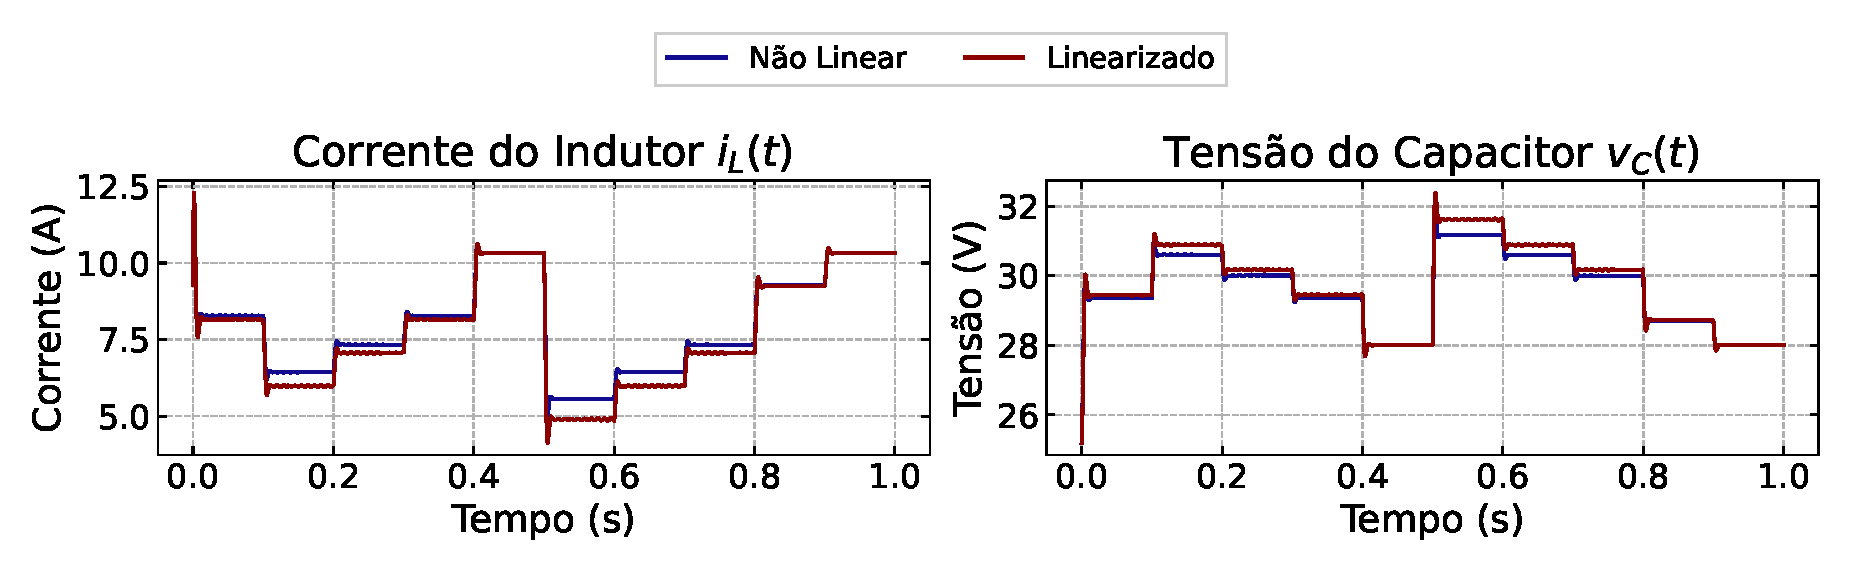
\includegraphics[width=1.\textwidth]{figuras/dynamic-etm/buck/sim2/op2/result.eps}
    \caption{Estados do conversor.}
    \label{fig:buck_converter_variable_pcpl_dynamic_etm_op2_a}
  \end{subfigure}
  \\[6pt]
  \begin{subfigure}{1.\textwidth}
    \centering
    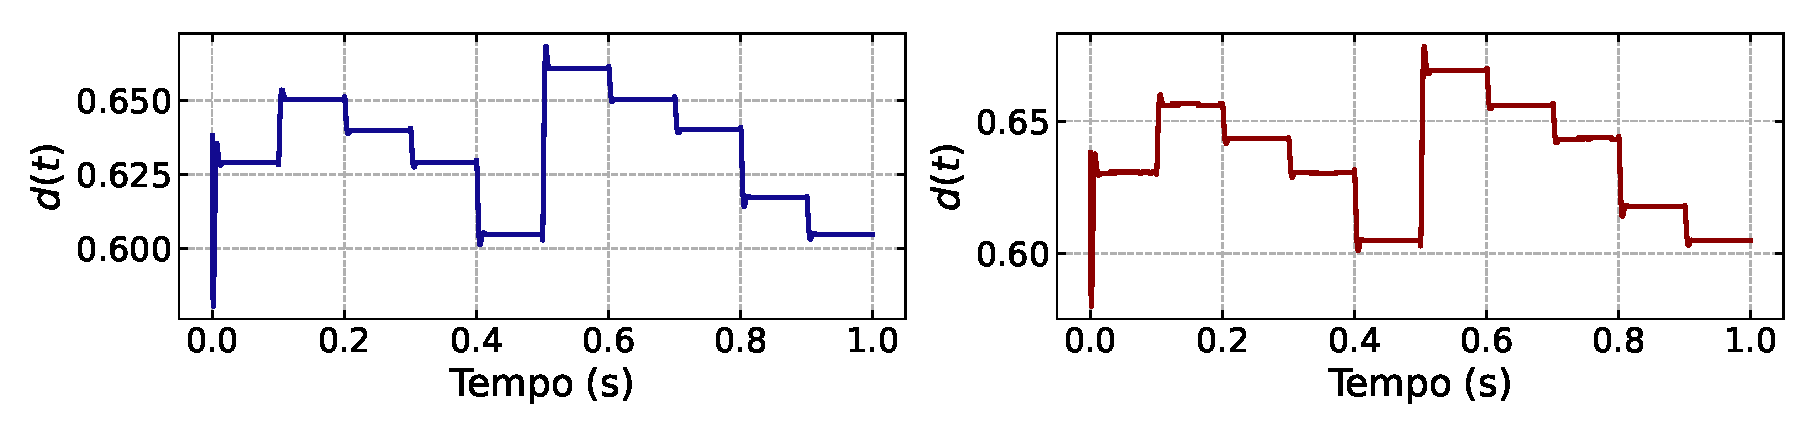
\includegraphics[width=1.\textwidth]{figuras/dynamic-etm/buck/sim2/op2/duty-cycle.eps}
    \caption{Duty Cycle $d(t)$}
    \label{fig:buck_converter_variable_pcpl_dynamic_etm_op2_b}
  \end{subfigure}
  \\[6pt]
  \begin{subfigure}{1.\textwidth}
    \centering
    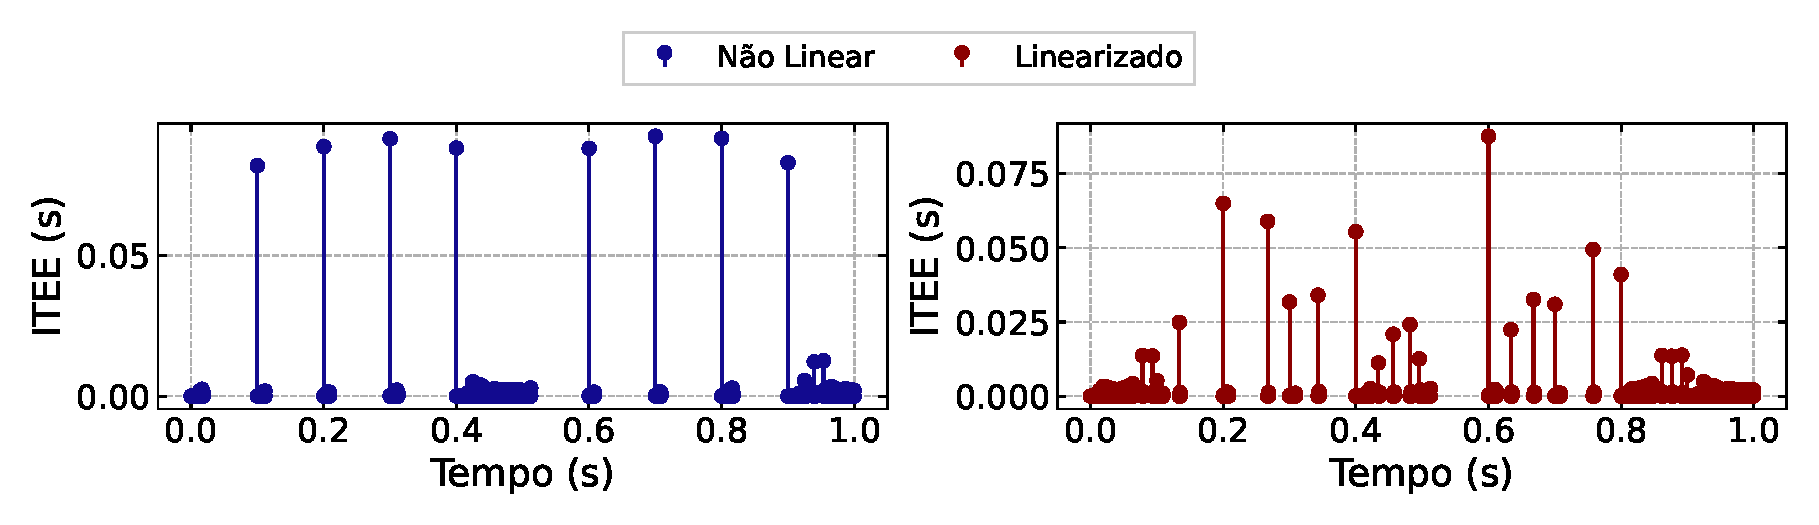
\includegraphics[width=1.\textwidth]{figuras/dynamic-etm/buck/sim2/op2/inter-event-times.eps}
    \caption{Intervalo de tempo entre eventos.}
    \label{fig:buck_converter_variable_pcpl_dynamic_etm_op2_c}
  \end{subfigure}
  \caption{Estados $i_L(t)$, $v_C(t)$ e $\eta(t)$, a entrada duty cycle $d(t)$ e os \acrshortpl{itee} do conversor Buck em torno do ponto $P_{\mathrm{o}, 2}$ sob sinal de pertubação $P_{\mathrm{cpl}}(t)$ variável e \acrshort{etm} estático.}
  \label{fig:buck_converter_variable_pcpl_dynamic_etm_op2}
\end{figure}

No entanto, ao considerar os pontos instáveis, como $P_{\mathrm{o}, 2}$, os intervalos entre eventos aumentam consideravelmente, indicando uma redução na frequência de ocorrências em comparação com a simulação utilizando o \acrshort{etm} estático. Nesses casos, a variável dinâmica não converge para a origem quando a perturbação se afasta do ponto de operação, como pode ser observado na \autoref{fig:buck_converter_variable_pcpl_dynamic_etm_eta}. Apesar disso, o \acrshort{etm} dinâmico assegura a estabilidade global do sistema ao longo de toda a simulação, mantendo-o dentro de limites aceitáveis de operação.

\begin{figure}[H]
  \centering
  \captionsetup{justification=centering}
  \begin{subfigure}{1.\textwidth}
    \centering
    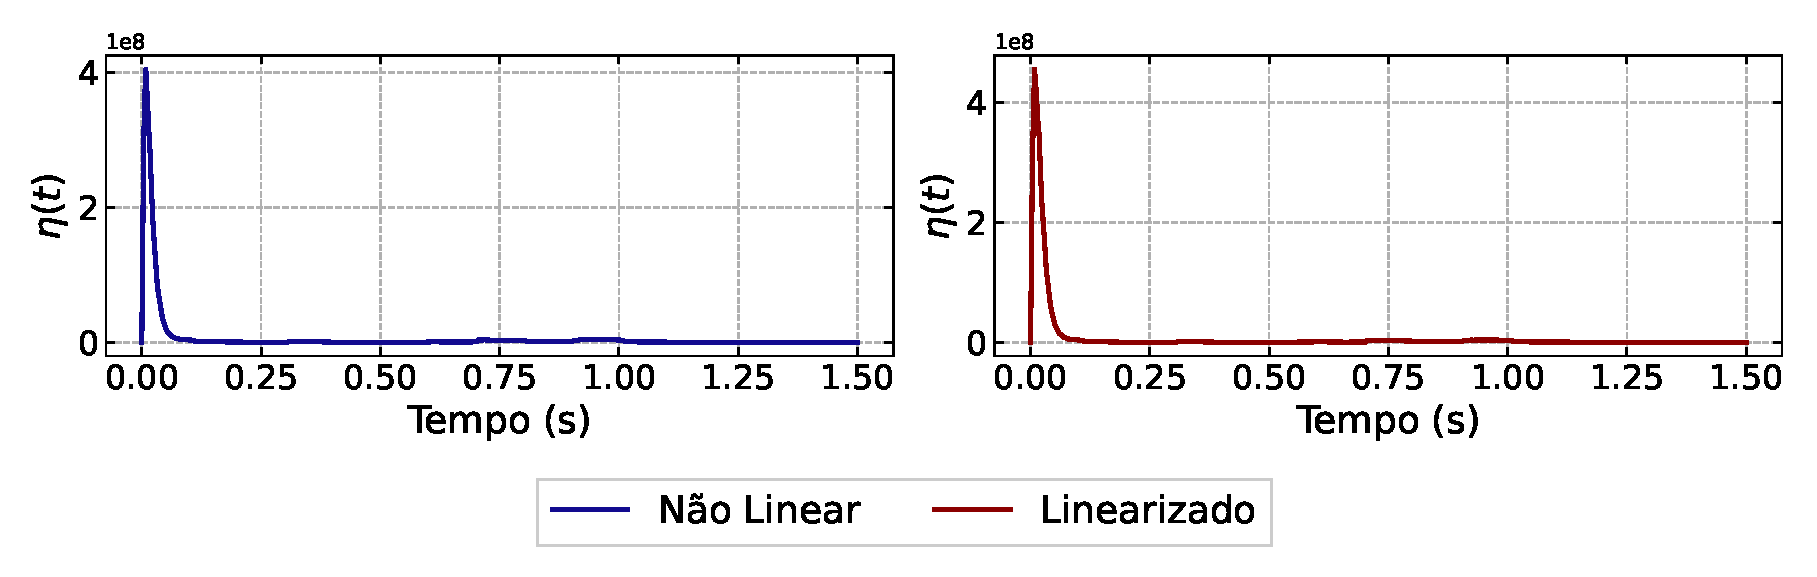
\includegraphics[width=1.\textwidth]{figuras/dynamic-etm/buck/sim2/op1/eta.eps}
    \caption{Ponto de operação $P_{\mathrm{o}, 1}$}
    \label{fig:buck_converter_variable_pcpl_dynamic_etm_eta_a}
  \end{subfigure}
  \\[6pt]
  \begin{subfigure}{1.\textwidth}
    \centering
    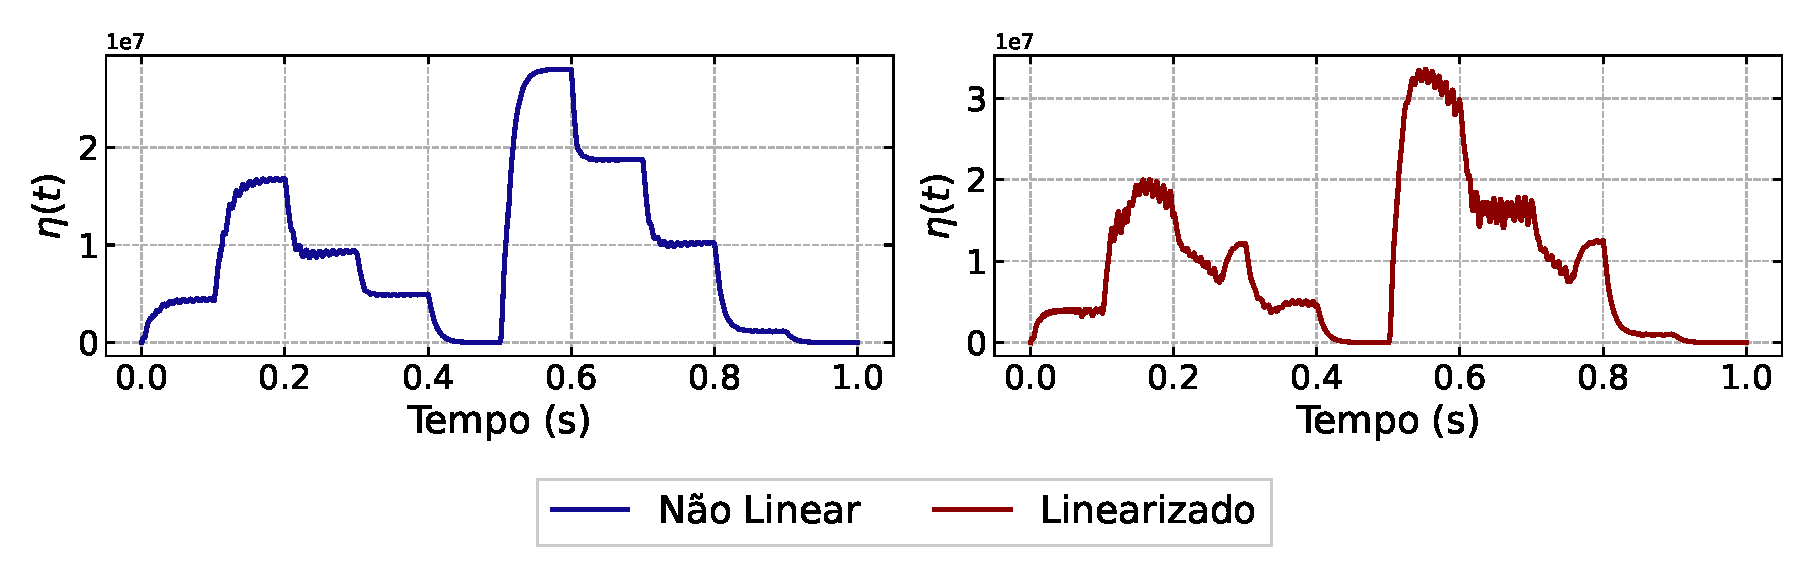
\includegraphics[width=1.\textwidth]{figuras/dynamic-etm/buck/sim2/op2/eta.eps}
    \caption{Ponto de operação $P_{\mathrm{o}, 2}$}
    \label{fig:buck_converter_variable_pcpl_dynamic_etm_eta_b}

  \end{subfigure}
  \caption{Variável dinâmica $\eta(t)$ do \acrshort{etm} dinâmico sob sinal de pertubação $P_{\mathrm{cpl}}(t)$ variável.}
  \label{fig:buck_converter_variable_pcpl_dynamic_etm_eta}
\end{figure}

As Figuras \ref{fig:classic_buck_cen2_op1} e \ref{fig:classic_buck_cen2_op2} demonstram o comportamento do conversor Buck no Cenário 2, submetido por um controlador projetado conforme o critério de estabilidade de Hurwitz. É possível observar uma significativa diferença do desempenho do sistema em relação ao uso do \acrshort{etm}. Sob este controlador, o sistema exibe múltiplas oscilações, contrastando com o comportamento mais estável do \acrshort{etm}. Além disso, a resposta do sistema ainda permanece mais lenta em comparação com o \acrshort{etm}.

\begin{figure}[H]
  \centering
  \captionsetup{justification=centering}
  \begin{subfigure}{1.\textwidth}
    \centering
    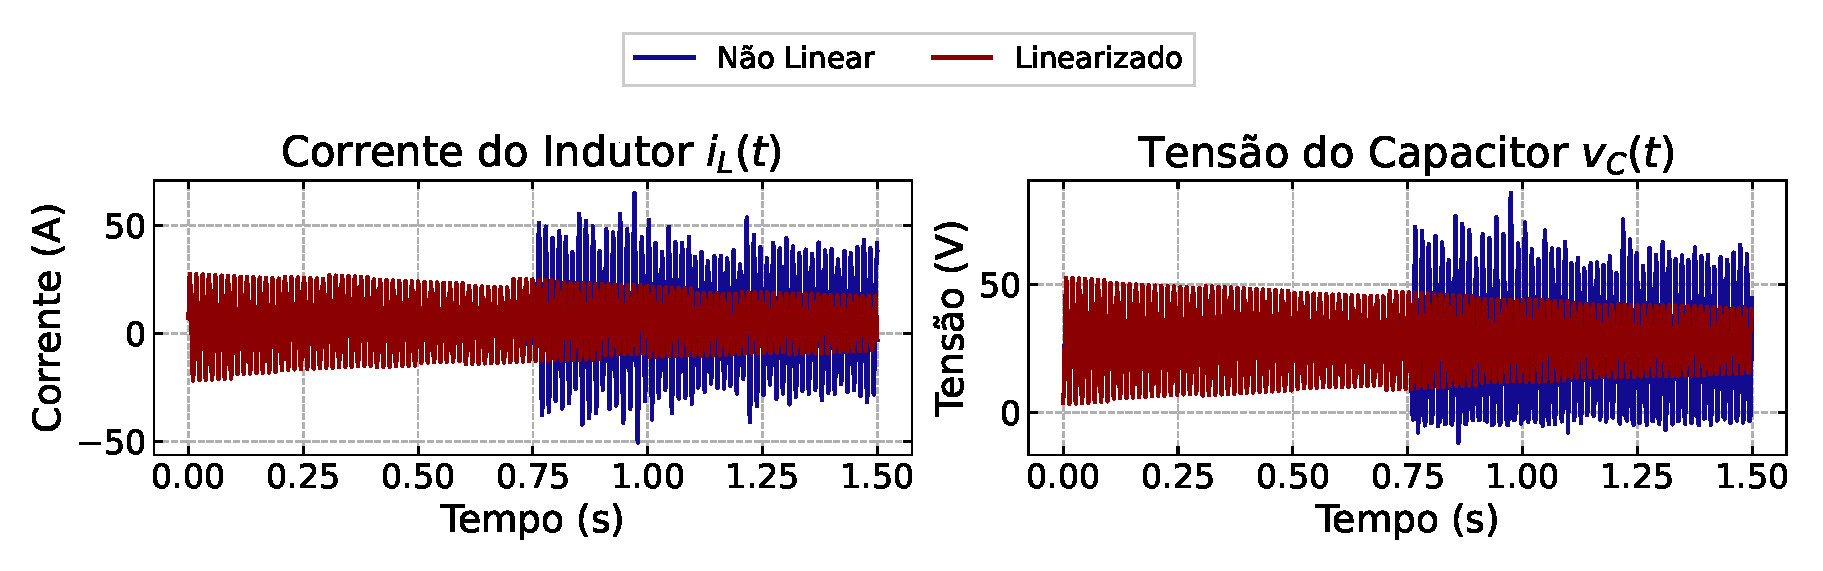
\includegraphics[width=1.\textwidth]{figuras/classic/buck/sim2/op1/result.eps}
    \caption{Estados do Sistema $i_L(t)$  e $v_C(t)$}
  \end{subfigure}
  \\[6pt]
  \begin{subfigure}{1.\textwidth}
    \centering
    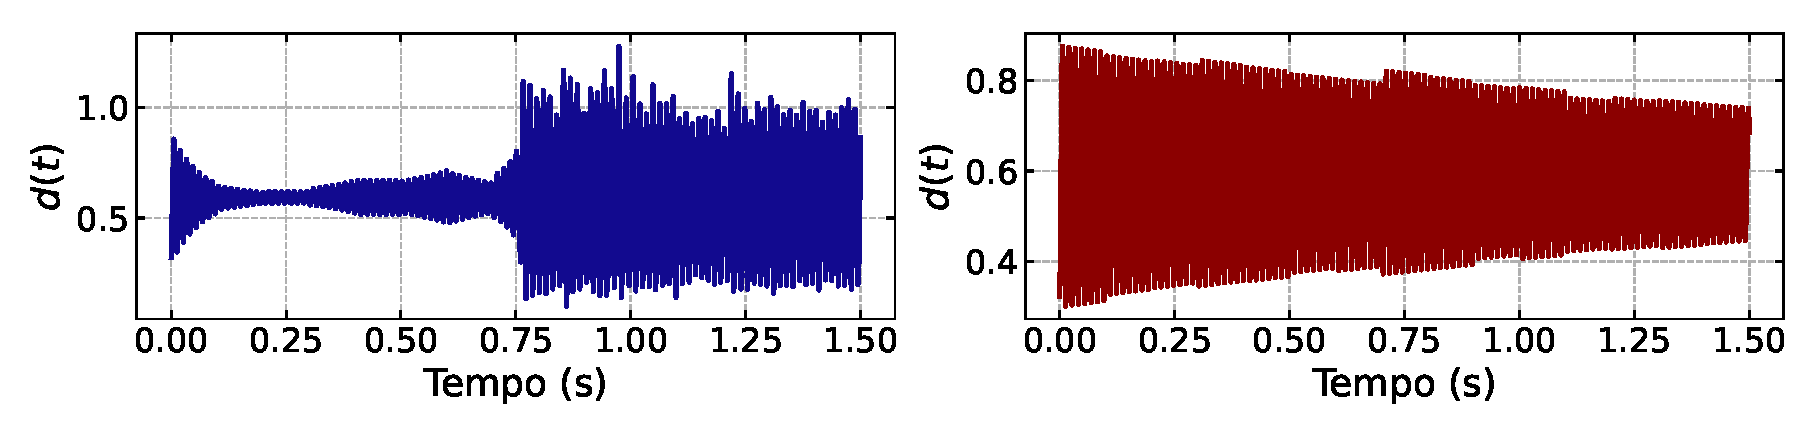
\includegraphics[width=1.\textwidth]{figuras/classic/buck/sim2/op1/duty-cycle.eps}
    \caption{Entrada controlável do Sistema $d(t)$}
  \end{subfigure}
  \caption{Conversor Buck no Cenário 2 operando em torno de $P_{\mathrm{o}, 1}$ sob controlador projetado utilizando o critério de estabilidade de Hurwitz.}
  \label{fig:classic_buck_cen2_op1}
  \begin{subfigure}{1.\textwidth}
    \centering
    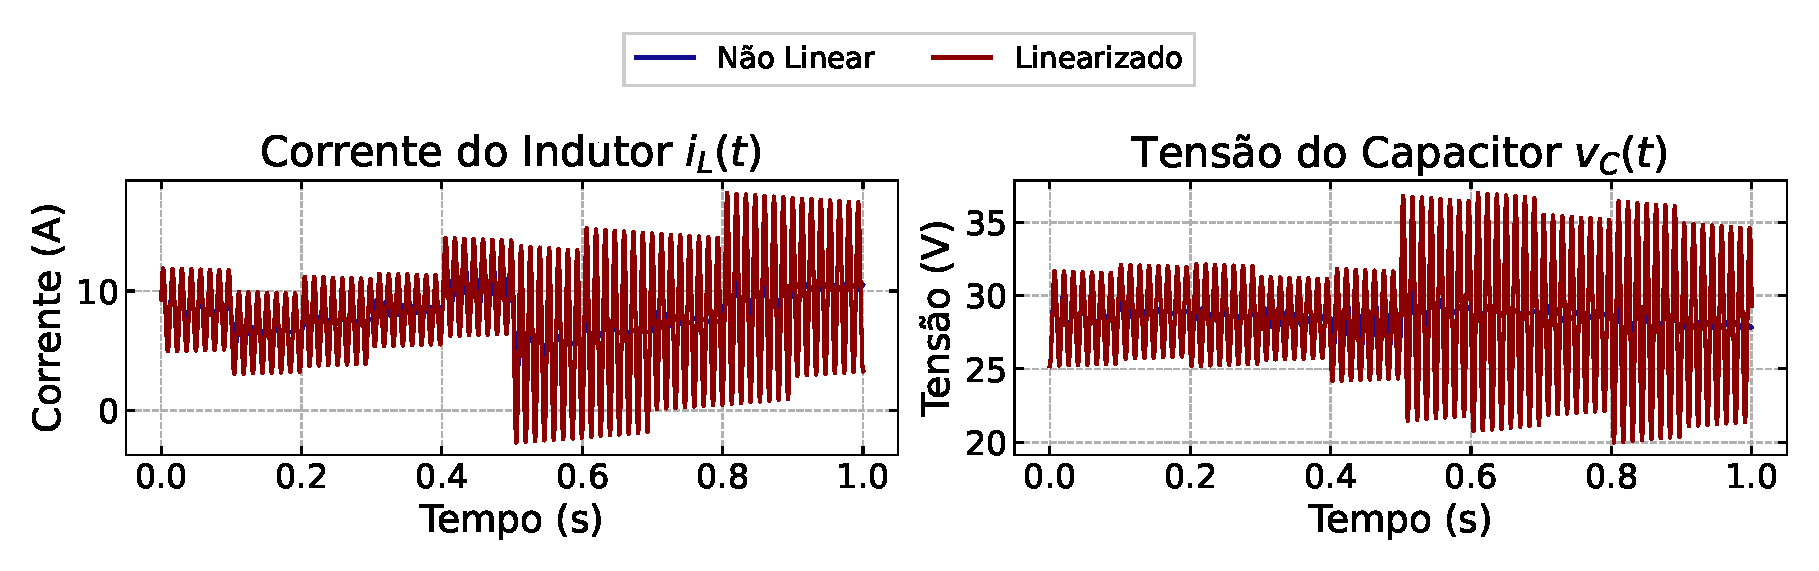
\includegraphics[width=1.\textwidth]{figuras/classic/buck/sim2/op2/result.eps}
    \caption{Estados do Sistema $i_L(t)$  e $v_C(t)$}
  \end{subfigure}
  \\[6pt]
  \begin{subfigure}{1.\textwidth}
    \centering
    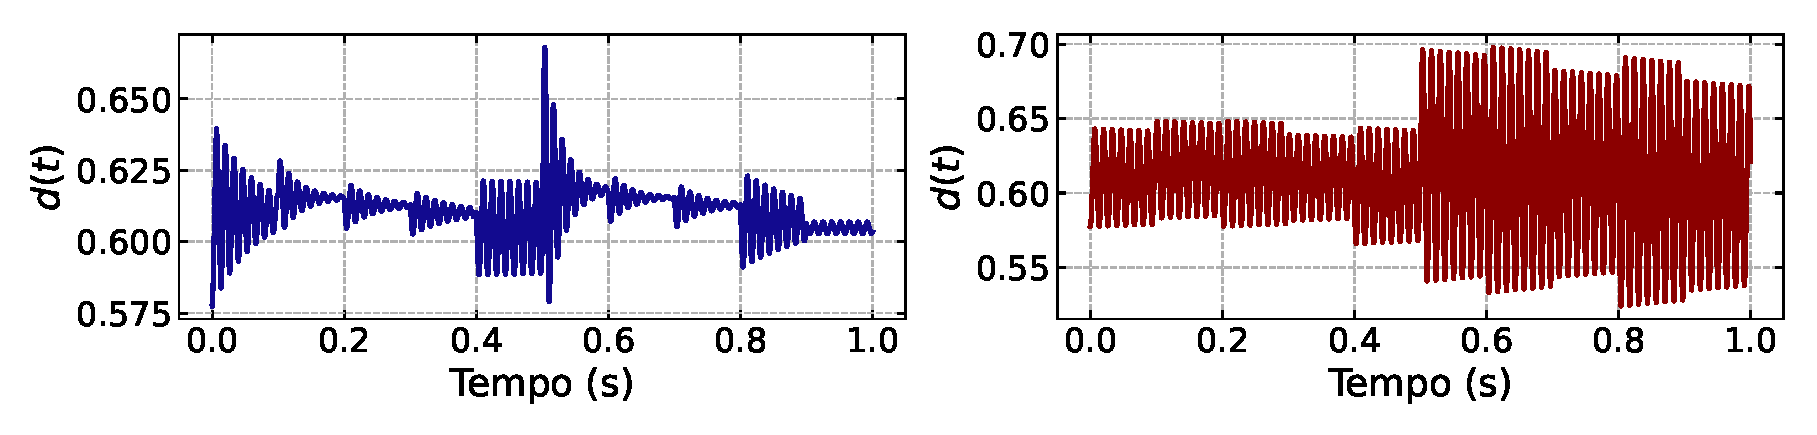
\includegraphics[width=1.\textwidth]{figuras/classic/buck/sim2/op2/duty-cycle.eps}
    \caption{Entrada controlável do Sistema $d(t)$}
  \end{subfigure}
  \caption{Conversor Buck no Cenário 2 em torno de $P_{\mathrm{o}, 2}$ sob controlador projetado utilizando o critério de estabilidade de Hurwitz.}
  \label{fig:classic_buck_cen2_op2}
\end{figure}


\subsubsection{Análise Numérica de Desempenho}

A \autoref{table:imees_buck_static_dynamic} apresenta as médias dos \acrshortpl{itee} obtidas durante a simulação do conversor Buck sob os \acrshort{etm} dinâmico e estático. Ao analisar os resultados para o ponto de operação $P_{\mathrm{o}, 1}$, observa-se que a diferença entre os \acrshortpl{itee} obtidos com o ETM estático e dinâmico não é expressiva. Isso indica que, neste ponto de operação, o ETM estático já apresenta um desempenho satisfatório. No entanto, no ponto de operação $P_{\mathrm{o}, 2}$, os \acrshortpl{itee} obtidos com o ETM dinâmico são consideravelmente superiores aos do ETM estático. Essa diferença evidencia a capacidade do ETM dinâmico em reduzir o número de eventos acionados. Os resultados demonstram que o ETM dinâmico apresenta um desempenho superior ao ETM estático ao reduzir o número de eventos.

\vspace{12pt}
\begin{table}[H]
  \centering
  \captionsetup{justification=centering}
  \setlength{\tabcolsep}{10pt}
  \begin{tabular}{cccccccc}
    \toprule
    \multirow{2}{*}{\centering Cenário} & \multirow{2}{*}{\centering \acrshort{po}} & \multicolumn{2}{c}{\centering Modelo} & \multirow{2}{*}{\centering Cenário} & \multirow{2}{*}{\centering \acrshort{po}} & \multicolumn{2}{c}{\centering Modelo}                     \\
    \cmidrule(lr){3-4} \cmidrule(lr){7-8}                      &                                           & NL                                    & L                                   &                                           &                                       & NL      & L       \\
    \midrule
    1                                   & $P_{\mathrm{o}, 1}$                       & 0,28 ms                               & 0,26 ms                             & 1                                         & $P_{\mathrm{o}, 1}$                   & 0,29 ms & 0,16 ms \\
    2                                   & $P_{\mathrm{o}, 1}$                       & 0,60 ms                               & 0,42 ms                             & 2                                         & $P_{\mathrm{o}, 1}$                   & 0,60 ms & 0,60 ms \\
    1                                   & $P_{\mathrm{o}, 2}$                       & 7,67 $\mu$s                           & 7,64 $\mu$s                         & 1                                         & $P_{\mathrm{o}, 2}$                   & 0,06 ms & 0,06 ms \\
    2                                   & $P_{\mathrm{o}, 2}$                       & 39,19 $\mu$s                          & 38,89 $\mu$s                        & 2                                         & $P_{\mathrm{o}, 2}$                   & 0,24 ms & 0,22 ms \\
    \bottomrule
  \end{tabular}
  \caption{\acrshortpl{imee} do conversor Buck sob \acrshort{etm} estático (à esquerda) e dinâmico (à direita).}
  \label{table:imees_buck_static_dynamic}
\end{table}

As Tabelas \ref{table:indices_desempenho_etm_estático} e \ref{table:indices_desempenho_etm_dinamico} detalham os tempos de acomodação, os \acrshortpl{ise}, os \acrshortpl{itse} e os \acrshortpl{isc} do conversor Buck operando no Cenário 1, tanto no contexto do \acrshort{etm} estático quanto no dinâmico, considerando a saída $v_C(t)$ do conversor e a entrada $d(t)$ determinada pelo controlador. Notavelmente, os valores obtidos são praticamente idênticos em ambas as configurações, sugerindo que não há diferenças significativas entre a saída $v_C(t)$ e a entrada $d(t)$ quando o conversor opera sob o \acrshort{etm} dinâmico ou estático. Além disso, observa-se que o controlador apresenta um acúmulo de esforço semelhante em todos os casos. 

\vspace{8pt}
\begin{table}[H]
  \centering
  \captionsetup{justification=centering}
  \setlength{\tabcolsep}{10pt}
  \begin{tabular}{ccccccc}
    \toprule
    Cenário & Modelo      & Tempo de acomodação & \acrshort{ise} & \acrshort{itse}       & \acrshort{isc} \\
    \midrule
    1       & NL  & 99,99 ms            & 3,98           & 0,04                  & 0,04           \\
    1       & L & 99,99 ms            & 2,57           & 0,02                  & 0,04           \\
    2       & NL  & 3,35 ms             & 0,02           & 21,70 $\cdot 10^{-6}$ & 0,04           \\
    2       & L & 3,30 ms             & 0,02           & 20,40 $\cdot 10^{-6}$ & 0,04           \\
    \bottomrule
  \end{tabular}
  \caption{Tempo de acomodação, \acrshort{ise}, \acrshort{itse} e \acrshort{isc} do conversor Buck sob \acrshort{etm} estático.}
  \label{table:indices_desempenho_etm_estático}
\end{table}

\vspace{8pt}
\begin{table}[H]
  \centering
  \captionsetup{justification=centering}
  \setlength{\tabcolsep}{10pt}
  \begin{tabular}{ccccccc}
    \toprule
    Cenário & Modelo      & Tempo de acomodação & \acrshort{ise} & \acrshort{itse}       & \acrshort{isc} \\
    \midrule
    1       & NL  & 100,00 ms           & 3,98           & 0,04                  & 0,04           \\
    1       & L & 100,00 ms           & 2,57           & 0,02                  & 0,04           \\
    2       & NL  & 3,35 ms             & 0,02           & 21,70 $\cdot 10^{-6}$ & 0,04           \\
    2       & L & 3,30 ms             & 0,02           & 20,40 $\cdot 10^{-6}$ & 0,04           \\
    \bottomrule
  \end{tabular}
  \caption{Tempo de acomodação, \acrshort{ise}, \acrshort{itse} e \acrshort{isc} do conversor Buck sob \acrshort{etm} dinâmico.}
  \label{table:indices_desempenho_etm_dinamico}
\end{table}

\subsection{Conversor Boost}

O conversor Boost, que anteriormente passou por análise em malha aberta conforme descrito na \autoref{section:open_loop}, foi submetido a simulações em malha fechada, mantendo as mesmas condições de operação. A avaliação foi realizada em dois pontos de operação distintos, $P_{\mathrm{o}, 3}$ e $P_{\mathrm{o}, 4}$, em duas situações diferentes: uma com o sinal de perturbação $P_{\mathrm{cpl}}$ mantido constante e outra com variação desse sinal. Os pontos de operação e os sinais de perturbação utilizados nas duas situações são idênticos aos utilizados na análise em malha aberta.

No desenvolvimento do \acrshort{etm} para as simulações com o sinal de perturbação mantido constante e variável, adotou-se o valor constante $\mu = 0,5$. Os parâmetros de projeto obtidos do problema de otimização multiobjetivo para o conversor Boost em torno do ponto de operação $P_{\mathrm{o}, 3}$ são os seguintes: \begin{gather}
  \Xi = \begin{bmatrix}
    4,30 \cdot 10^5  & -3,26 \cdot 10^4 \\
    -3,26 \cdot 10^4 & 2,01 \cdot 10^6  \\
  \end{bmatrix}, \hspace{.5cm}
  \Psi = \begin{bmatrix}
    1,51 \cdot 10^8    & 1,03 \cdot 10^{-6} \\
    1,03 \cdot 10^{-6} & 1,77 \cdot 10^8    \\
  \end{bmatrix} \text{ e } \notag \\[12pt]
  K = \begin{bmatrix}
    -2,81 \cdot 10^{-7} & 3,08 \cdot 10^{-8}
  \end{bmatrix} . \notag
\end{gather} E, para o conversor em torno do ponto $P_{\mathrm{o}, 4}$, os parâmetros são: \begin{gather}
  \Xi = \begin{bmatrix}
    2,77\cdot 10^{13} & 1,03\cdot 10^{13} \\
    1,03\cdot 10^{13} & 1,12\cdot 10^{13} \\
  \end{bmatrix}, \hspace{.5cm}
  \Psi = \begin{bmatrix}
    6,18\cdot 10^{8}  & 4,44\cdot 10^{-5} \\
    4,44\cdot 10^{-5} & 6,17\cdot 10^{8}  \\
  \end{bmatrix} \text{ e } \notag \\[12pt]
  K = \begin{bmatrix}
    -2,24 \cdot 10^{-2} & -7,45\cdot 10^{-3}
  \end{bmatrix} . \notag
\end{gather} Os parâmetros $\theta$ e $\lambda$ da lei de acionamento dos \acrshortpl{etm} dinâmicos utilizados nas simulações foram estabelecidos como 0.1 e 100, respectivamente.

\subsubsection{Cenário 1}

Na simulação em malha aberta, a análise mostrou que conversor Boost em torno dos pontos de operação $P_{\mathrm{o}, 3}$ apresentava estabilidade, enquanto que em torno do ponto $P_{\mathrm{o}, 4}$ apresentava instabilidade. No entanto, ao considerarmos o comportamento do conversor em malha fechada com o \acrshort{etm} estático, observa-se uma estabilização em ambos os pontos, conforme apresentado na \autoref{fig:boost_converter_constant_pcpl_static_etm_op1_duty_a} e \autoref{fig:boost_converter_constant_pcpl_static_etm_op2_duty_a}. 

\begin{figure}[H]
  \centering
  \captionsetup{justification=centering}
  \begin{subfigure}{1.\textwidth}
    \centering
    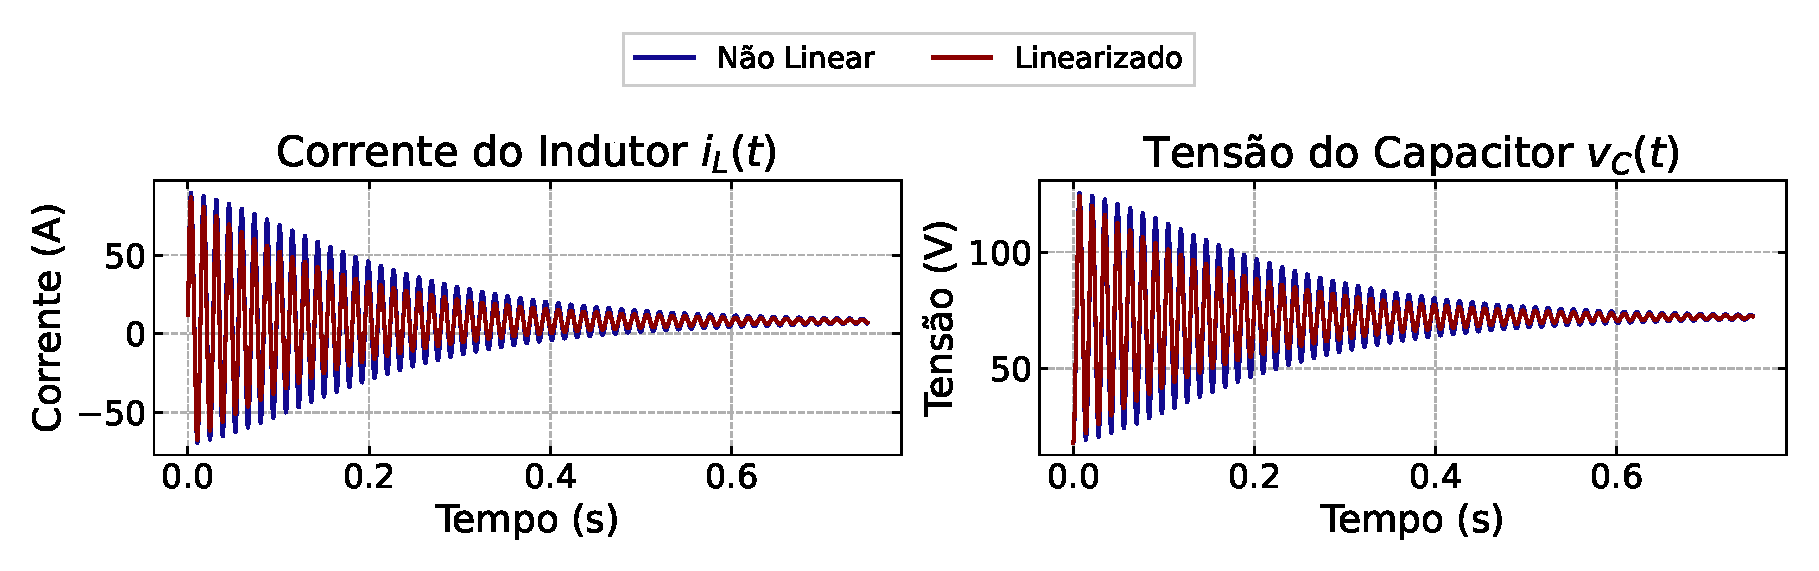
\includegraphics[width=1.\textwidth]{figuras/static-etm/boost/sim1/op1/result.eps}
    \caption{Estados do conversor.}
    \label{fig:boost_converter_constant_pcpl_static_etm_op1_duty_a}
  \end{subfigure}
  \\[6pt]
  \begin{subfigure}{1.\textwidth}
    \centering
    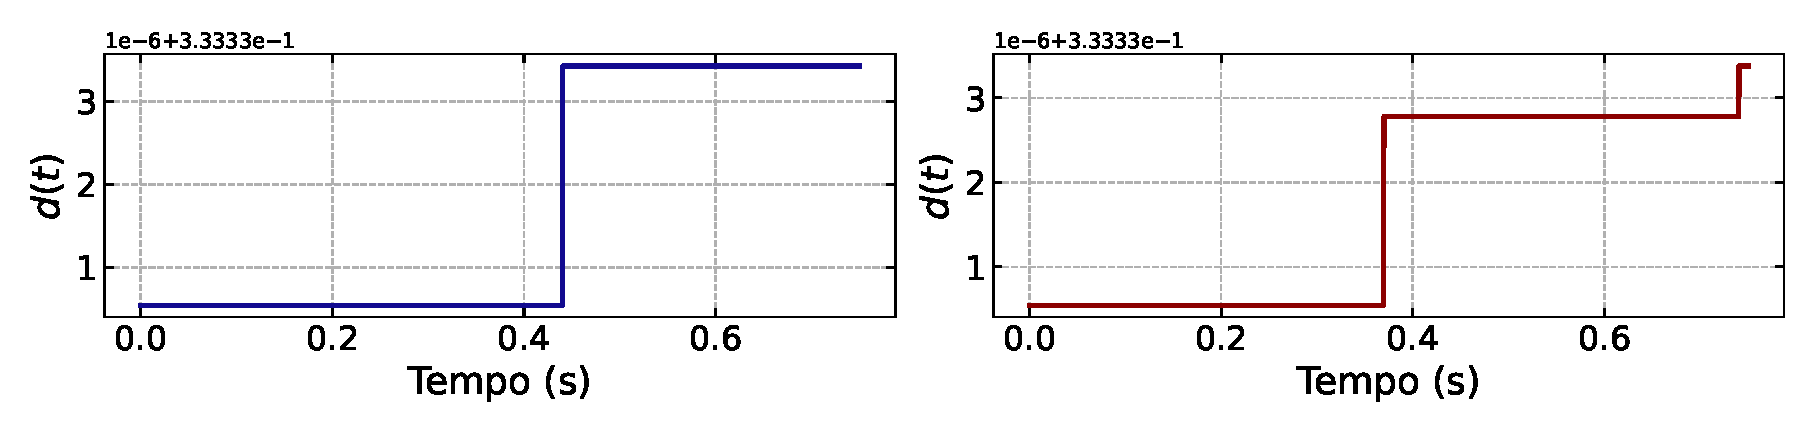
\includegraphics[width=1.\textwidth]{figuras/static-etm/boost/sim1/op1/duty-cycle.eps}
    \caption{Duty Cycle $d(t)$}
    \label{fig:boost_converter_constant_pcpl_static_etm_op1_duty_b}
  \end{subfigure}
  \\[6pt]
  \begin{subfigure}{1.\textwidth}
    \centering
    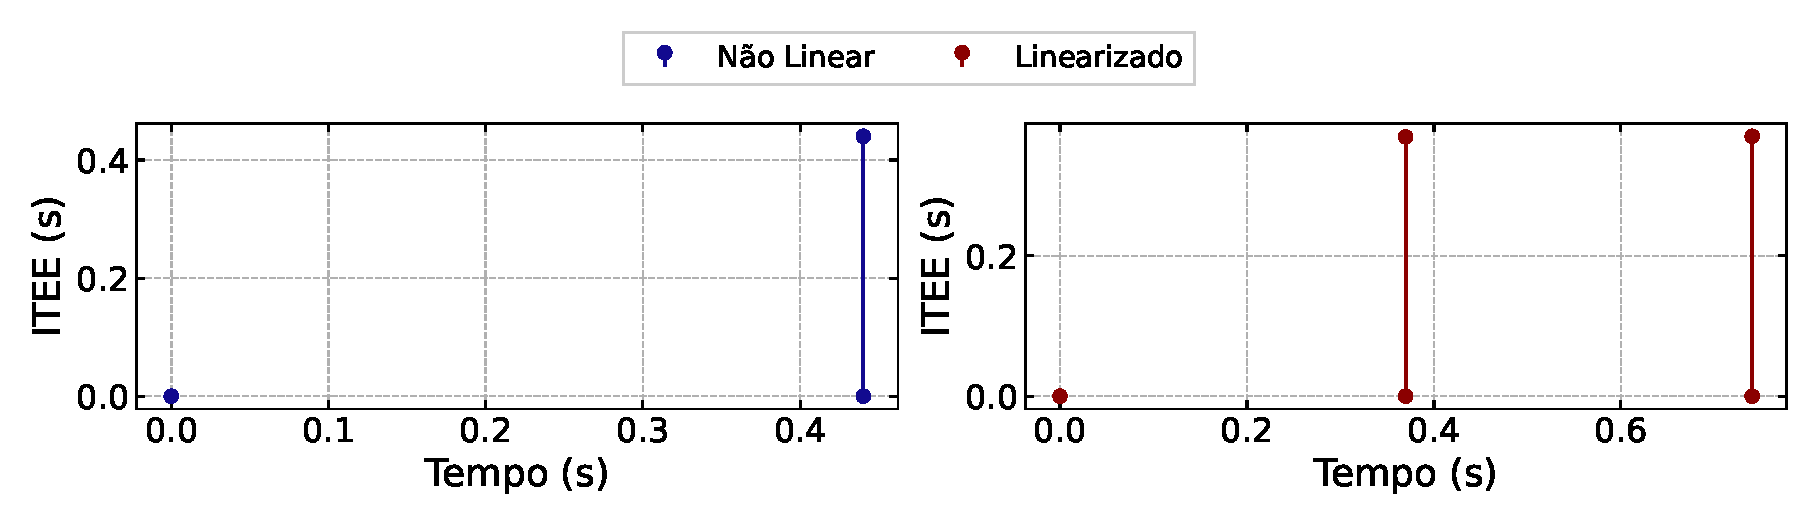
\includegraphics[width=1.\textwidth]{figuras/static-etm/boost/sim1/op1/inter-event-times.eps}
    \caption{Intervalo de tempo entre eventos.}
    \label{fig:boost_converter_constant_pcpl_static_etm_op1_duty_c}
  \end{subfigure}
  \caption{Estados $i_L(t)$ e $v_C(t)$, a entrada duty cycle $d(t)$ e os \acrshortpl{itee} do conversor Boost em torno do ponto $P_{\mathrm{o}, 3}$ sob sinal de pertubação $P_{\mathrm{cpl}}(t)$ constante e \acrshort{etm} estático.}
\end{figure}

Em $P_{\mathrm{o}, 3}$, não houve diferenças significativas entre os comportamentos em malha aberta e fechada. Já em $P_{\mathrm{o}, 4}$, embora os modelos linear e não linear tenham divergido em malha aberta, a estabilidade foi alcançada em malha fechada, com ambos os modelos se alinhando ao ponto de operação definido. Durante a simulação do conversor em torno de $P_{\mathrm{o}, 3}$ (\autoref{fig:boost_converter_constant_pcpl_static_etm_op1_duty_c}), foram necessários apenas dois eventos no modelo não linear e três eventos no modelo linearizado, durante todo o período de simulação, resultando em maiores intervalos de tempo entre os eventos. Entretanto, a variação causada na entrada duty cycle é bastante pequena em torno do ponto de operação do duty cycle, da ordem de $10^{-6}$. Essa pequena variação não causa mudanças significativas no sistema, o que justifica a semelhança observada com o sistema em malha aberta nessas circunstâncias.

\begin{figure}[H]
  \centering
  \captionsetup{justification=centering}
  \begin{subfigure}{1.\textwidth}
    \centering
    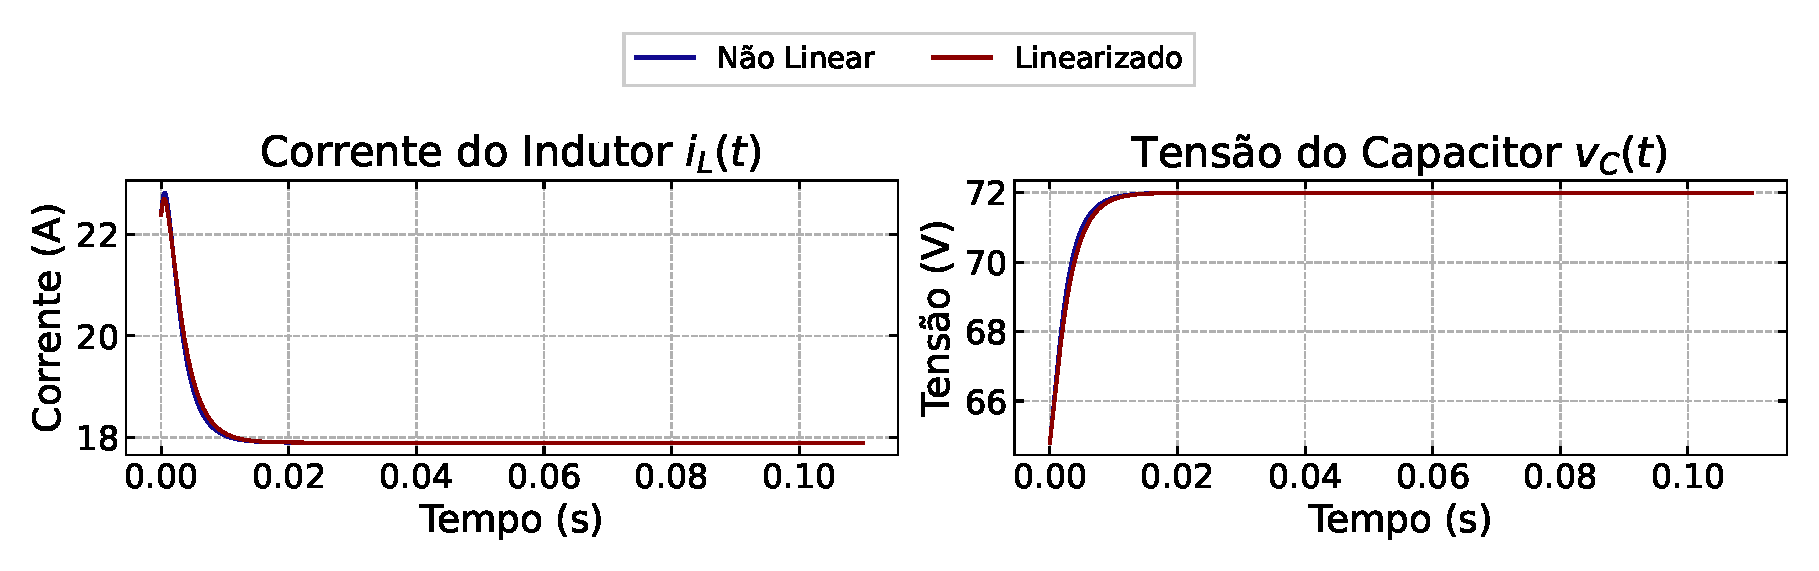
\includegraphics[width=1.\textwidth]{figuras/static-etm/boost/sim1/op2/result.eps}
    \caption{Estados do conversor.}
    \label{fig:boost_converter_constant_pcpl_static_etm_op2_duty_a}
  \end{subfigure}
  \\[6pt]
  \begin{subfigure}{1.\textwidth}
    \centering
    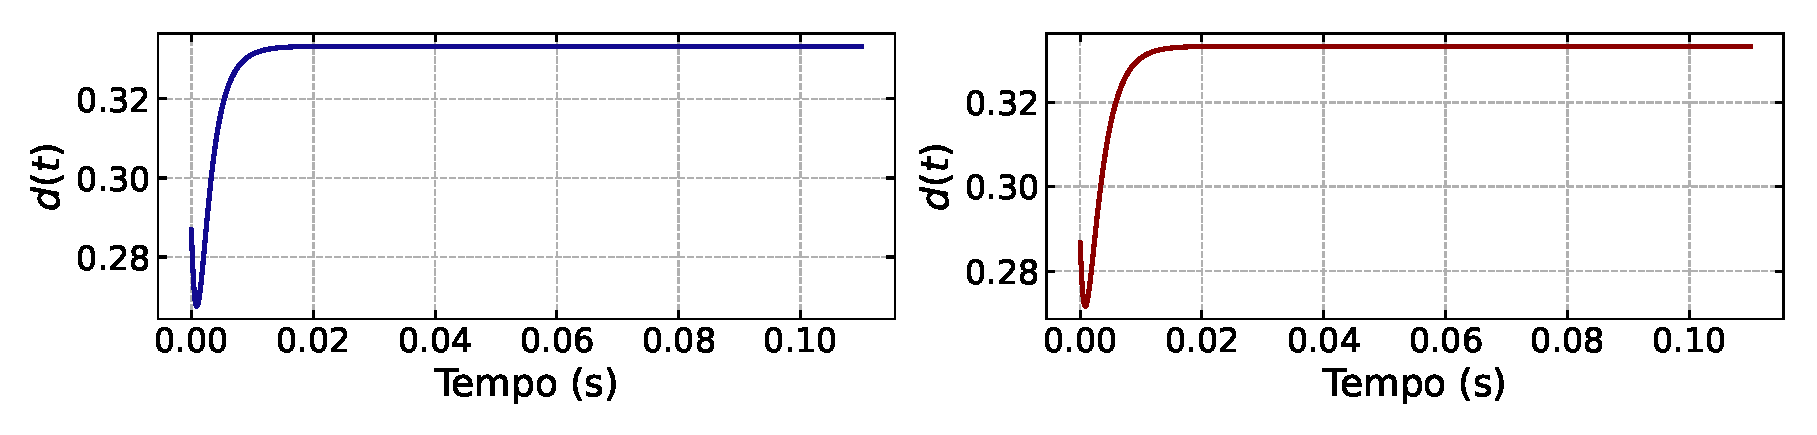
\includegraphics[width=1.\textwidth]{figuras/static-etm/boost/sim1/op2/duty-cycle.eps}
    \caption{Duty Cycle $d(t)$}
    \label{fig:boost_converter_constant_pcpl_static_etm_op2_duty_b}
  \end{subfigure}
  \\[6pt]
  \begin{subfigure}{1.\textwidth}
    \centering
    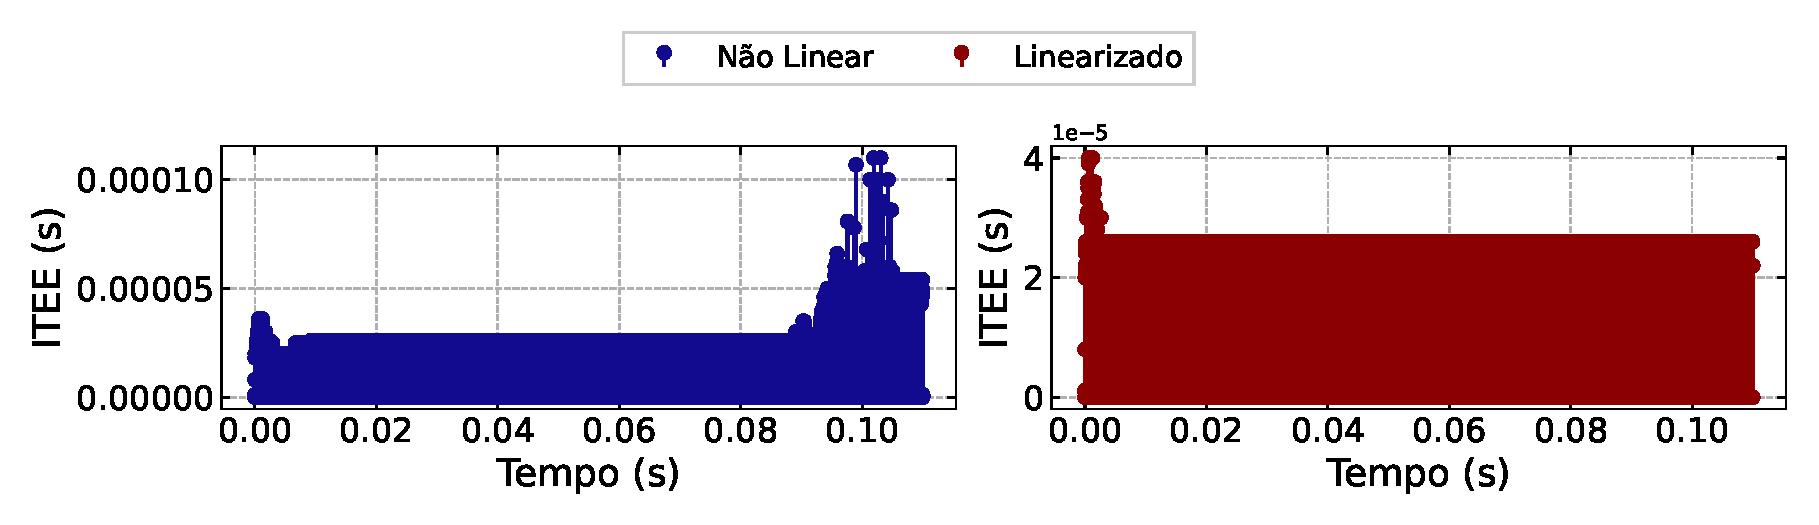
\includegraphics[width=1.\textwidth]{figuras/static-etm/boost/sim1/op2/inter-event-times.eps}
    \caption{Intervalo de tempo entre eventos.}
    \label{fig:boost_converter_constant_pcpl_static_etm_op2_duty_c}
  \end{subfigure}
  \caption{Estados $i_L(t)$ e $v_C(t)$, a entrada duty cycle $d(t)$ e os \acrshortpl{itee} do conversor Boost em torno do ponto $P_{\mathrm{o}, 4}$ sob sinal de pertubação $P_{\mathrm{cpl}}(t)$ constante e \acrshort{etm} estático.}
\end{figure}

A simulação do conversor Boost em torno do ponto instável $P_{\mathrm{o}, 4}$ revelou um comportamento similar ao do conversor Buck (\autoref{fig:boost_converter_constant_pcpl_static_etm_op2_duty_c}). O \acrshort{etm} gerou sucessivos eventos devido à instabilidade inerente a este ponto de operação. À medida que o sistema tende a se desviar gradualmente, o erro de transmissão aumenta, tornando a função de acionamento do \acrshort{etm}  negativa e permitindo o disparo de novos eventos. Esse ciclo pode se repetir mesmo após a estabilização do sistema em malha fechada, justificando a contínua atuação do \acrshort{etm}.

\begin{figure}[H]
  \centering
  \captionsetup{justification=centering}
  \begin{subfigure}{1.\textwidth}
    \centering
    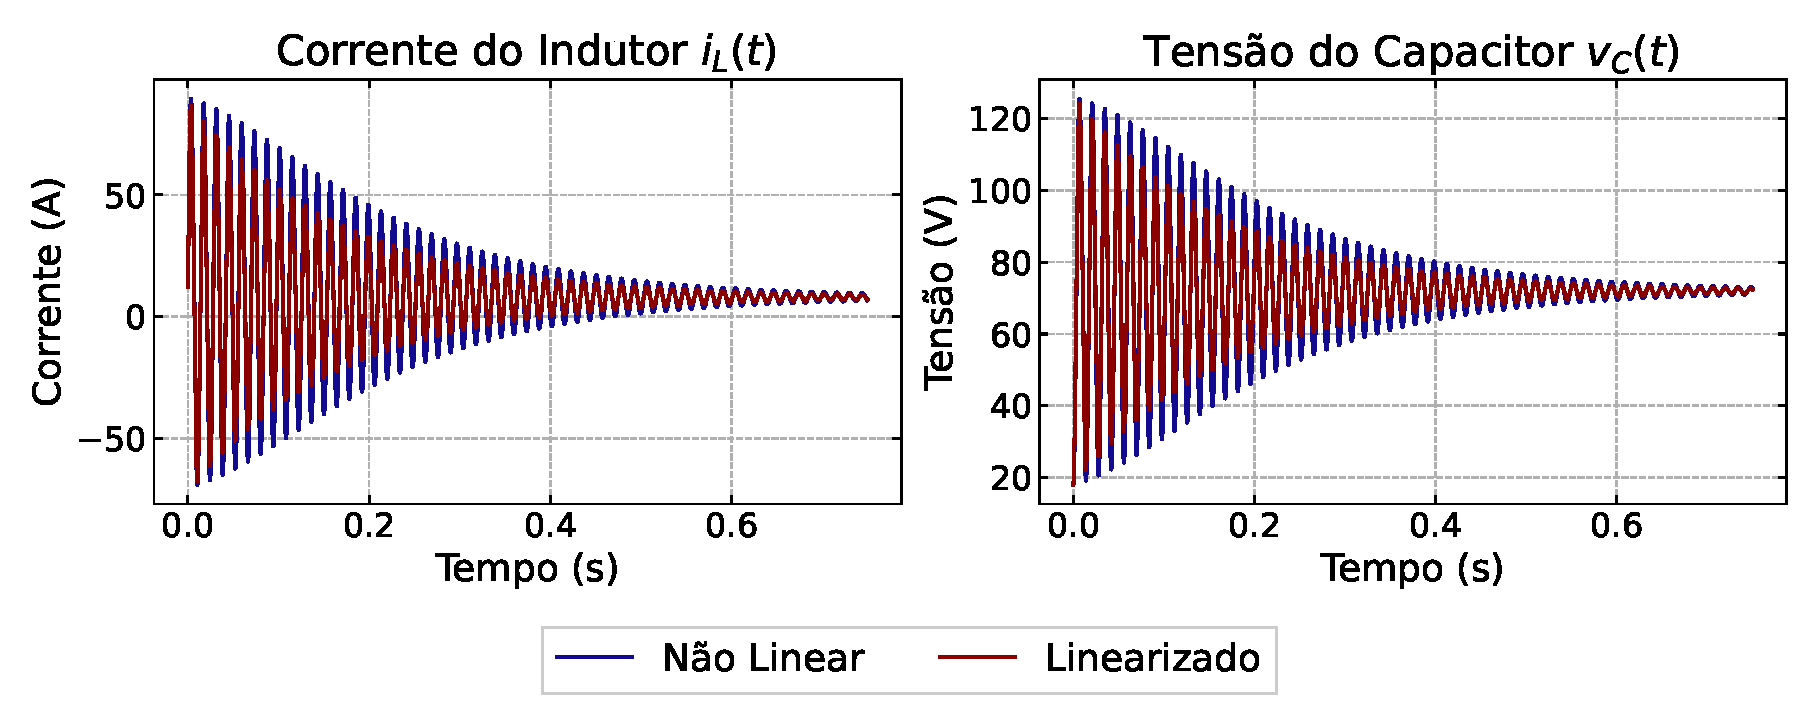
\includegraphics[width=1.\textwidth]{figuras/dynamic-etm/boost/sim1/op1/result.eps}
    \caption{Estados do conversor.}
    \label{fig:boost_converter_constant_pcpl_dynamic_etm_op1_a}
  \end{subfigure}
  \\[6pt]
  \begin{subfigure}{1.\textwidth}
    \centering
    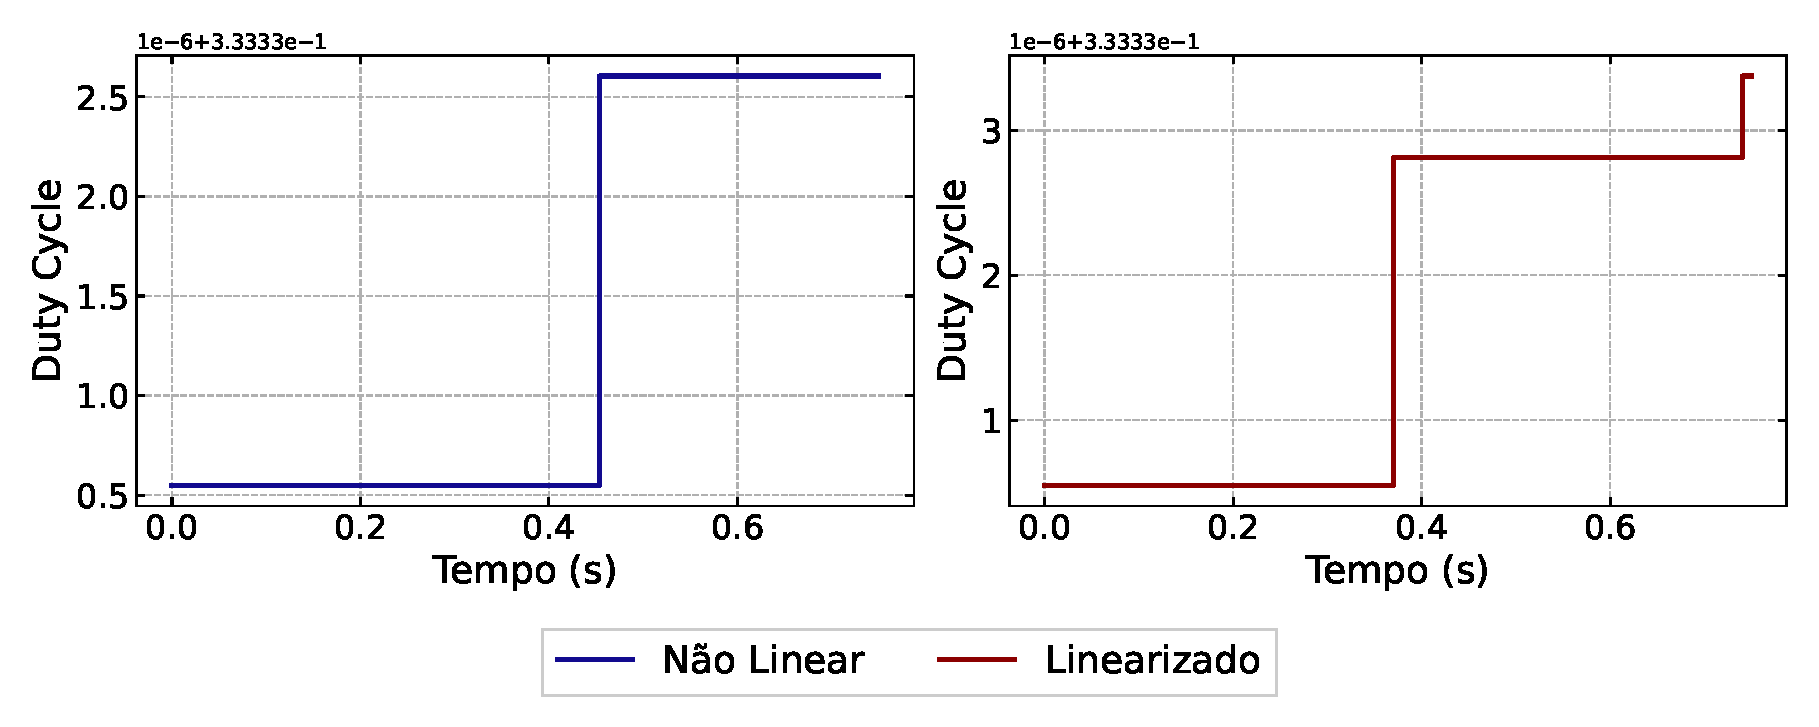
\includegraphics[width=1.\textwidth]{figuras/dynamic-etm/boost/sim1/op1/duty-cycle.eps}
    \caption{Duty Cycle $d(t)$}
    \label{fig:boost_converter_constant_pcpl_dynamic_etm_op1_b}
  \end{subfigure}
  \\[6pt]
  \begin{subfigure}{1.\textwidth}
    \centering
    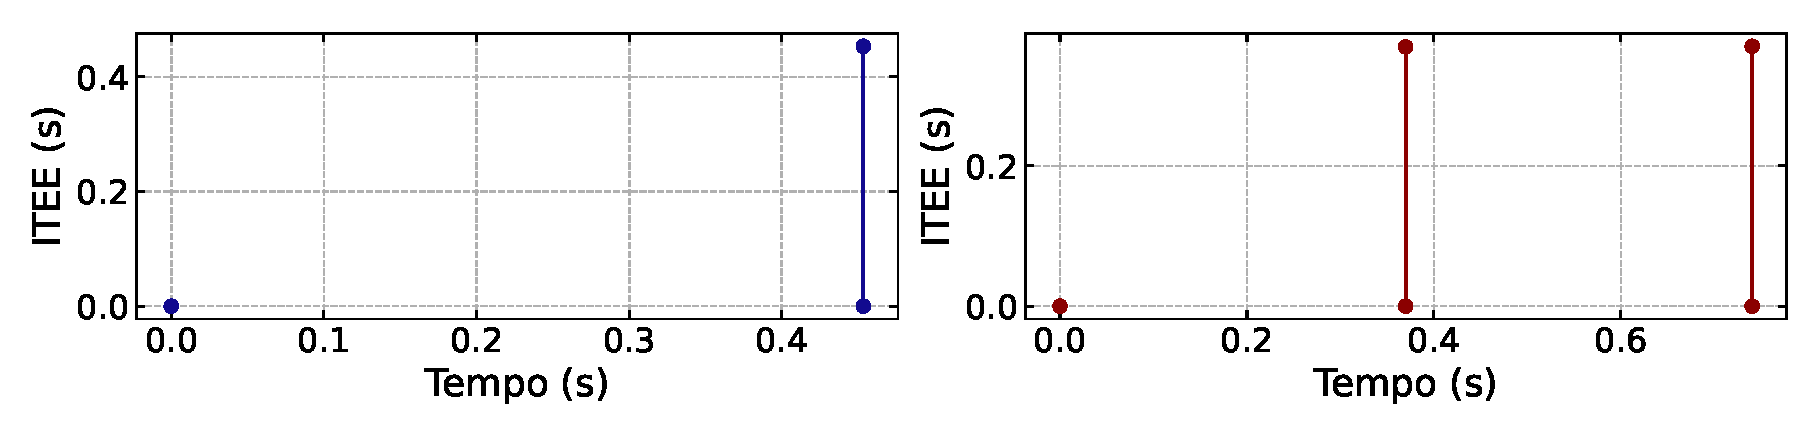
\includegraphics[width=1.\textwidth]{figuras/dynamic-etm/boost/sim1/op1/inter-event-times.eps}
    \caption{Intervalo de tempo entre eventos.}
    \label{fig:boost_converter_constant_pcpl_dynamic_etm_op1_c}
  \end{subfigure}
  \caption{Estados $i_L(t)$, $v_C(t)$ e $\eta(t)$, a entrada duty cycle $d(t)$ e os \acrshortpl{itee} do conversor boost em torno do ponto $P_{\mathrm{o}, 1}$ sob sinal de pertubação $P_{\mathrm{cpl}}(t)$ constante e \acrshort{etm} estático.}
  \label{fig:boost_converter_constant_pcpl_dynamic_etm_op1}
\end{figure}

\begin{figure}[H]
  \centering
  \captionsetup{justification=centering}
  \begin{subfigure}{1.\textwidth}
    \centering
    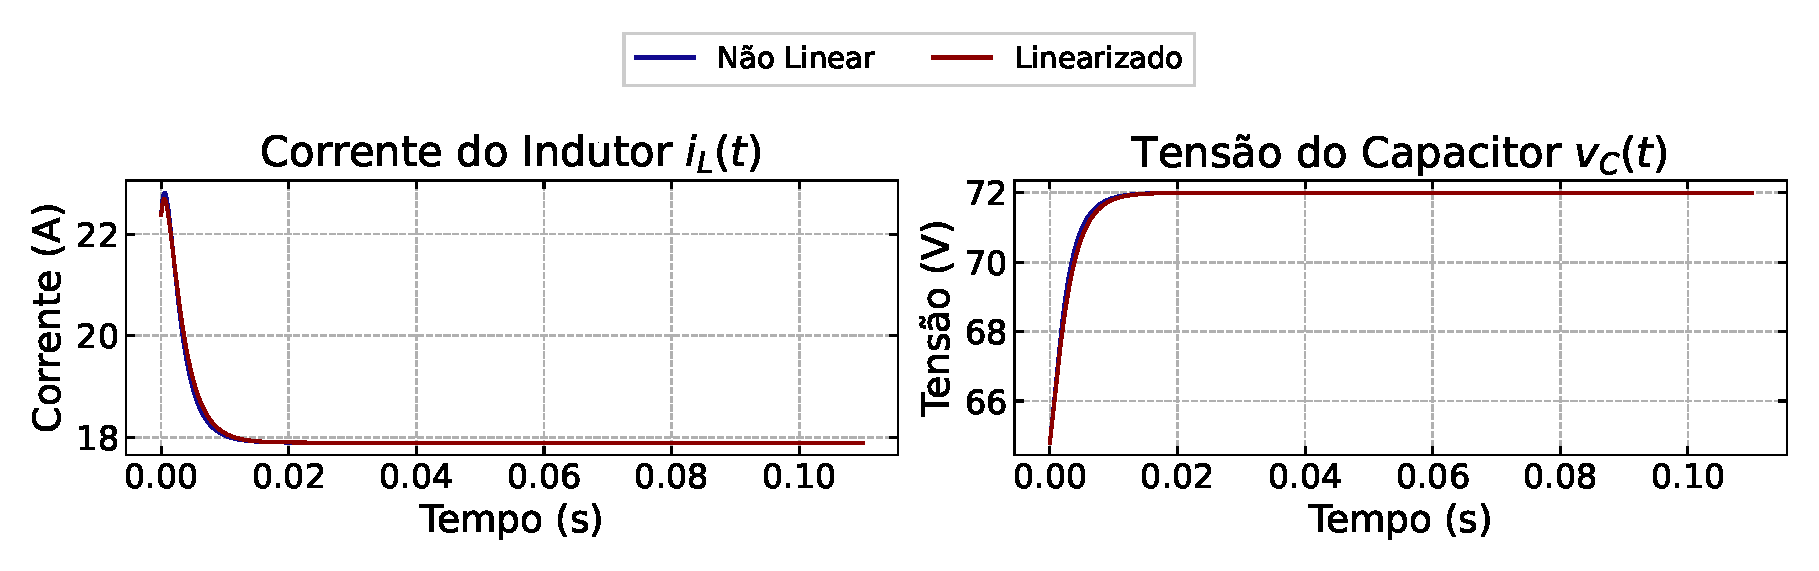
\includegraphics[width=1.\textwidth]{figuras/dynamic-etm/boost/sim1/op2/result.eps}
    \caption{Estados do conversor.}
    \label{fig:boost_converter_constant_pcpl_dynamic_etm_op2_a}
  \end{subfigure}
  \\[6pt]
  \begin{subfigure}{1.\textwidth}
    \centering
    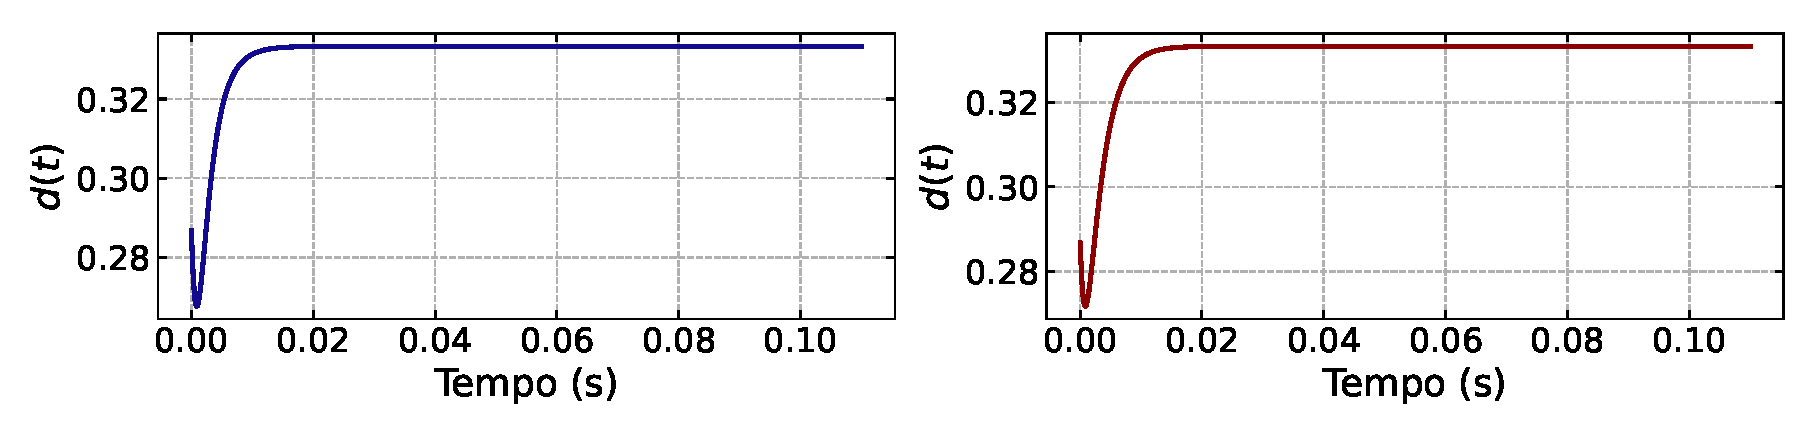
\includegraphics[width=1.\textwidth]{figuras/dynamic-etm/boost/sim1/op2/duty-cycle.eps}
    \caption{Duty Cycle $d(t)$}
    \label{fig:boost_converter_constant_pcpl_dynamic_etm_op2_b}
  \end{subfigure}
  \\[6pt]
  \begin{subfigure}{1.\textwidth}
    \centering
    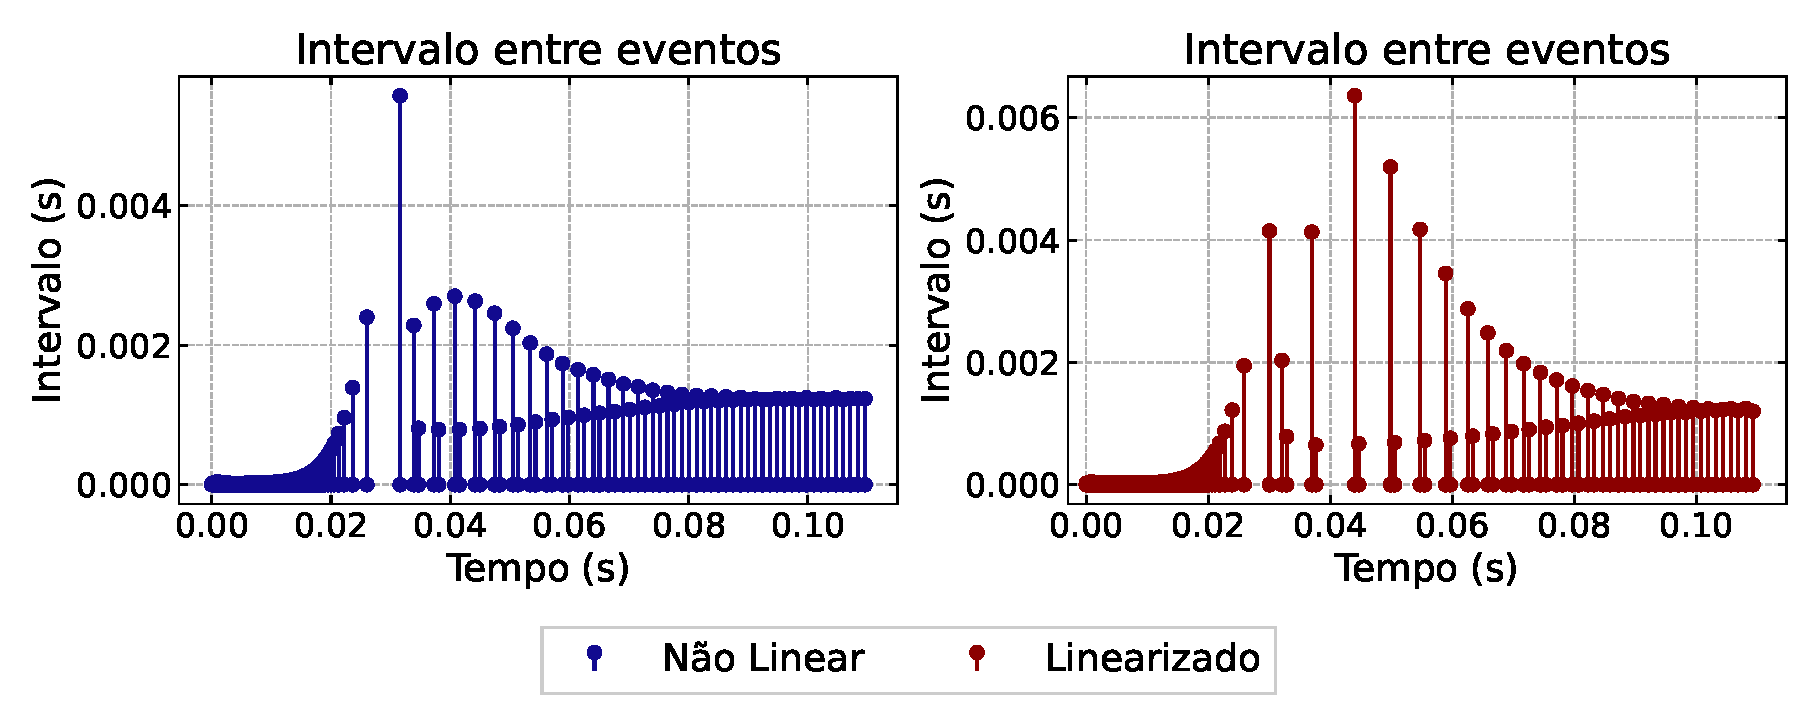
\includegraphics[width=1.\textwidth]{figuras/dynamic-etm/boost/sim1/op2/inter-event-times.eps}
    \caption{Intervalo de tempo entre eventos.}
    \label{fig:boost_converter_constant_pcpl_dynamic_etm_op2_c}
  \end{subfigure}
  \caption{Estados $i_L(t)$, $v_C(t)$ e $\eta(t)$, a entrada duty cycle $d(t)$ e os \acrshortpl{itee} do conversor boost em torno do ponto $P_{\mathrm{o}, 2}$ sob sinal de pertubação $P_{\mathrm{cpl}}(t)$ constante e \acrshort{etm} estático.}
  \label{fig:boost_converter_constant_pcpl_dynamic_etm_op2}
\end{figure}

No contexto do \acrshort{etm} dinâmico, ao analisar o comportamento do conversor Boost, nota-se uma semelhança entre o desempenho do \acrshort{etm} dinâmico e estático em torno do ponto $P_{\mathrm{o}, 3}$, como indicado pelas Figuras \ref{fig:boost_converter_constant_pcpl_dynamic_etm_op1_a}, \ref{fig:boost_converter_constant_pcpl_dynamic_etm_op1_b} e \ref{fig:boost_converter_constant_pcpl_dynamic_etm_op1_c}. Não foram observadas discrepâncias significativas nessas condições. No entanto, ao examinar a distribuição de eventos perturbadores, observamos uma diferença marcante na Figura \ref{fig:boost_converter_constant_pcpl_dynamic_etm_op1_c}. Com o \acrshort{etm} dinâmico, houve uma redução significativa na quantidade de eventos, com uma distribuição mais uniforme ao longo do tempo, em contraste com a concentração de eventos vista com o \acrshort{etm} estático. Essa uniformidade na distribuição de eventos sugere uma maior estabilidade e controle do sistema, destacando a eficácia do \acrshort{etm} dinâmico em cenários de perturbação constante no contexto de conversores Boost.

\begin{figure}[H]
  \centering
  \captionsetup{justification=centering}
  \begin{subfigure}{1.\textwidth}
    \centering
    \includegraphics[width=1.\textwidth]{figuras/dynamic-etm/boost/sim1/op1/eta.eps}
    \caption{Ponto de operação $P_{\mathrm{o}, 1}$}
  \end{subfigure}
  \\[6pt]
  \begin{subfigure}{1.\textwidth}
    \centering
    \includegraphics[width=1.\textwidth]{figuras/dynamic-etm/boost/sim1/op2/eta.eps}
    \caption{Ponto de operação $P_{\mathrm{o}, 2}$}
  \end{subfigure}
  \caption{Variável dinâmica $\eta(t)$ do \acrshort{etm} dinâmico sob sinal de pertubação $P_{\mathrm{cpl}}(t)$ constante.}
  \label{fig:boost_converter_constant_pcpl_dynamic_etm_eta}
\end{figure}

Na \autoref{fig:boost_converter_constant_pcpl_dynamic_etm_eta}, é mostrada as variações temporais de $\eta(n)$ durante a simulação do conversor Boost em operações estáveis e instáveis, no Cenário 1. Observa-se que $\eta(t)$ permanece não negativa e converge para o equilíbrio na origem. Esse comportamento resulta em um aumento nos \acrshortpl{itee}, conforme evidenciado pela comparação entre as operações estáveis e instáveis.

A \autoref{fig:boost_converter_mu} apresenta os resultados obtidos ao variar o parâmetro $\rho$ da função objetivo do problema de otimização \eqref{eq:optimization_problem}. Conforme $\rho$ aumenta, observa-se uma diminuição gradual na média dos \acrshortpl{itee}, aproximando-se de zero, enquanto os tempos de acomodação aumentam. Durante a simulação do conversor sob \acrshort{etm} dinâmico, notaram-se diferenças nas médias dos \acrshortpl{itee} entre o modelo não linear e o linearizado, especialmente para valores de $\rho$ entre 0 e 0,8. Nesse intervalo, o modelo linearizado registrou médias superiores em relação ao modelo não linear. Esta diferenças também podem ser observadas nas simulações anteriores, apresentadas nas Figuras \ref{fig:boost_converter_constant_pcpl_static_etm_op2_duty_c} e \ref{fig:boost_converter_constant_pcpl_dynamic_etm_op2_c}, onde, com $\rho = 0,5$, o modelo linear demonstrou acionar menos eventos em comparação ao modelo não linear. No \acrshort{etm} estático, as diferenças nas médias dos \acrshortpl{itee} não foram muito diferentes. Por outro lado, as médias dos \acrshortpl{itee} são maiores no \acrshort{etm} dinâmico que no estático. Além disso, os tempos de acomodação entre o \acrshort{etm} dinâmico e estático mostraram-se bastante semelhantes, assim como entre os modelos não linear e linearizado.

\begin{figure}[H]
  \centering
  \captionsetup{justification=centering}
  \begin{subfigure}{1.\textwidth}
    \centering
    \includegraphics[width=1.\textwidth]{figuras/boost/itee-mean.eps}
    \caption{Médias dos \acrshortpl{itee} em relação a variação de $\rho$}
  \end{subfigure}
  \\[6pt]
  \begin{subfigure}{1.\textwidth} 
    \centering
    \includegraphics[width=1.\textwidth]{figuras/boost/ts.eps}
    \caption{Os tempos de acomodação dos estados do sistema sob o \acrshort{etm} estático e dinâmico em resposta às mudanças em $\rho$.}
  \end{subfigure}
  \caption{Resposta do conversor Boost sob variação do parâmetro $\rho$.}
  \label{fig:boost_converter_mu}
\end{figure}

Nas Figuras \ref{fig:classic_boost_cen1_op1} e \ref{fig:classic_boost_cen1_op2}, é possível observar o comportamento do conversor Boost no Cenário 1, quando submetido a um controlador projetado com base no critério de estabilidade de Hurwitz. Em contrapartida ao \acrshort{etc}, no ponto de operação $P_{\mathrm{o}, 3}$, o sistema não linear não conseguiu estabilizar no ponto de operação estável, embora os demais modelos tenham mantido estabilidade. Além disso, em torno do ponto instável, o conversor apresentou várias oscilações, enquanto o \acrshort{etc} não demonstrou oscilações significativas.

\begin{figure}[H]
  \centering
  \captionsetup{justification=centering}
  \begin{subfigure}{1.\textwidth}
    \centering
    \includegraphics[width=1.\textwidth]{figuras/classic/boost/sim1/op1/result.eps}
    \caption{Estados do Sistema $i_L(t)$  e $v_C(t)$}
  \end{subfigure}
  \\[6pt]
  \begin{subfigure}{1.\textwidth}
    \centering
    \includegraphics[width=1.\textwidth]{figuras/classic/boost/sim1/op1/duty-cycle.eps}
    \caption{Entrada controlável do Sistema $d(t)$}
  \end{subfigure}
  \caption{Conversor Boost no Cenário 1 operando em torno de $P_{\mathrm{o}, 3}$ sob controlador projetado utilizando o critério de estabilidade de Hurwitz.}
  \label{fig:classic_boost_cen1_op1}
  \begin{subfigure}{1.\textwidth}
    \centering
    \includegraphics[width=1.\textwidth]{figuras/classic/boost/sim1/op2/result.eps}
    \caption{Estados do Sistema $i_L(t)$  e $v_C(t)$}
  \end{subfigure}
  \\[6pt]
  \begin{subfigure}{1.\textwidth}
    \centering
    \includegraphics[width=1.\textwidth]{figuras/classic/boost/sim1/op2/duty-cycle.eps}
    \caption{Entrada controlável do Sistema $d(t)$}
  \end{subfigure}
  \caption{Conversor Boost no Cenário 1 em torno de $P_{\mathrm{o}, 4}$ sob controlador projetado utilizando o critério de estabilidade de Hurwitz.}
  \label{fig:classic_boost_cen1_op2}
\end{figure}

\subsubsection{Cenário 2}

Na simulação do conversor Boost em malha fechada com perturbação variável, a mesma perturbação da simulação em malha aberta foi usada. O comportamento do conversor em torno do ponto $P_{\mathrm{o}, 3}$ foi similar em ambas as condições, com resposta rápida e poucos eventos, apesar das variações na perturbação, conforme apresentado na \autoref{fig:boost_converter_variable_pcpl_static_etm_op1_duty_a}. A pequena variação na entrada, da ordem de $10^{-6}$, não afetou significativamente o sistema, justificando a similaridade com a malha aberta. Isso ressalta a eficácia do \acrshort{etm} em manter a estabilidade da saída do conversor Boost no ponto de operação, mesmo sob perturbações.

\begin{figure}[H]
  \centering
  \captionsetup{justification=centering}
  \begin{subfigure}{1.\textwidth}
    \centering
    \includegraphics[width=1.\textwidth]{figuras/static-etm/boost/sim2/op1/result.eps}
    \caption{Estados do conversor.}
    \label{fig:boost_converter_variable_pcpl_static_etm_op1_duty_a}
  \end{subfigure}
  \\[6pt]
  \begin{subfigure}{1.\textwidth}
    \centering
    \includegraphics[width=1.\textwidth]{figuras/static-etm/boost/sim2/op1/duty-cycle.eps}
    \caption{Duty Cycle $d(t)$}
    \label{fig:boost_converter_variable_pcpl_static_etm_op1_duty_b}
  \end{subfigure}
  \\[6pt]
  \begin{subfigure}{1.\textwidth}
    \centering
    \includegraphics[width=1.\textwidth]{figuras/static-etm/boost/sim2/op1/inter-event-times.eps}
    \caption{Intervalo de tempo entre eventos.}
    \label{fig:boost_converter_variable_pcpl_static_etm_op1_duty_c}
  \end{subfigure}
  \caption{Estados $i_L(t)$ e $v_C(t)$, a entrada duty cycle $d(t)$ e os \acrshortpl{itee} do conversor Boost em torno do ponto $P_{\mathrm{o}, 3}$ sob sinal de pertubação $P_{\mathrm{cpl}}(t)$ variável e \acrshort{etm} estático.}
\end{figure}

O ETM estático assegurou a estabilidade do conversor Boost sob perturbação variável em torno do ponto de operação instável $P_{o, 4}$, conforme ilustrado na \autoref{fig:boost_converter_variable_pcpl_static_etm_op2_duty_a}. Apesar dos afastamentos da perturbação em determinados momentos em relação ao ponto de operação, não foram observadas diferenças significativas entre os modelos não linear e linearizado sob malha fechada, tornando-os praticamente idênticos. Embora haja semelhanças nos estados e na entrada do sistema, é evidente na \autoref{fig:boost_converter_variable_pcpl_static_etm_op2_duty_c} que os conjuntos de \acrshortpl{itee} são distintos entre o modelo não linear e o linearizado.

\begin{figure}[H]
  \centering
  \captionsetup{justification=centering}
  \begin{subfigure}{1.\textwidth}
    \centering
    \includegraphics[width=1.\textwidth]{figuras/static-etm/boost/sim2/op2/result.eps}
    \caption{Estados do conversor.}
    \label{fig:boost_converter_variable_pcpl_static_etm_op2_duty_a}
  \end{subfigure}
  \\[6pt]
  \begin{subfigure}{1.\textwidth}
    \centering
    \includegraphics[width=1.\textwidth]{figuras/static-etm/boost/sim2/op2/duty-cycle.eps}
    \caption{Duty Cycle $d(t)$}
    \label{fig:boost_converter_variable_pcpl_static_etm_op2_duty_b}
  \end{subfigure}
  \\[6pt]
  \begin{subfigure}{1.\textwidth}
    \centering
    \includegraphics[width=1.\textwidth]{figuras/static-etm/boost/sim2/op2/inter-event-times.eps}
    \caption{Intervalo de tempo entre eventos.}
    \label{fig:boost_converter_variable_pcpl_static_etm_op2_duty_c}
  \end{subfigure}
  \caption{Estados $i_L(t)$ e $v_C(t)$, a entrada duty cycle $d(t)$ e os \acrshortpl{itee} do conversor Boost em torno do ponto $P_{\mathrm{o}, 4}$ sob sinal de pertubação $P_{\mathrm{cpl}}(t)$ variável e \acrshort{etm} estático.}
\end{figure}

No contexto do \acrshort{etm} dinâmico, ao estudar o comportamento dos conversores Boost em situações de perturbação variável, notamos padrões semelhantes aos observados nos conversores Buck. Em torno dos pontos estáveis, como $P_{\mathrm{o}, 4}$ para o Boost (Figura \ref{fig:buck_converter_variable_pcpl_dynamic_etm_op2}), tanto o \acrshort{etm} dinâmico quanto o estático demonstram comportamentos comparáveis, com poucos novos eventos necessários para estabilização. No entanto, ao considerar pontos instáveis, os intervalos entre eventos aumentam, indicando uma menor frequência de ocorrências com o \acrshort{etm} dinâmico em comparação com o estático. Embora a variável dinâmica não convirja para a origem nessas situações, o \acrshort{etm} dinâmico garante a estabilidade global do sistema ao longo da simulação, mantendo-o operando dentro de limites aceitáveis e garantindo sua robustez diante de perturbações variáveis.

\begin{figure}[H]
  \centering
  \captionsetup{justification=centering}
  \begin{subfigure}{1.\textwidth}
    \centering
    \includegraphics[width=1.\textwidth]{figuras/dynamic-etm/boost/sim2/op1/result.eps}
    \caption{Estados do conversor.}
    \label{fig:boost_converter_variable_pcpl_dynamic_etm_op1_a}
  \end{subfigure}
  \\[6pt]
  \begin{subfigure}{1.\textwidth}
    \centering
    \includegraphics[width=1.\textwidth]{figuras/dynamic-etm/boost/sim2/op1/duty-cycle.eps}
    \caption{Duty Cycle $d(t)$}
    \label{fig:boost_converter_variable_pcpl_dynamic_etm_op1_b}
  \end{subfigure}
  \\[6pt]
  \begin{subfigure}{1.\textwidth}
    \centering
    \includegraphics[width=1.\textwidth]{figuras/dynamic-etm/boost/sim2/op1/inter-event-times.eps}
    \caption{Intervalo de tempo entre eventos.}
    \label{fig:boost_converter_variable_pcpl_dynamic_etm_op1_c}
  \end{subfigure}
  \caption{Estados $i_L(t)$, $v_C(t)$ e $\eta(t)$, a entrada duty cycle $d(t)$ e os \acrshortpl{itee} do conversor boost em torno do ponto $P_{\mathrm{o}, 1}$ sob sinal de pertubação $P_{\mathrm{cpl}}(t)$ variável e \acrshort{etm} estático.}
  \label{fig:boost_converter_variable_pcpl_dynamic_etm_op1}
\end{figure}

\begin{figure}[H]
  \centering
  \captionsetup{justification=centering}
  \begin{subfigure}{1.\textwidth}
    \centering
    \includegraphics[width=1.\textwidth]{figuras/dynamic-etm/boost/sim2/op2/result.eps}
    \caption{Estados do conversor.}
    \label{fig:boost_converter_variable_pcpl_dynamic_etm_op2_a}
  \end{subfigure}
  \\[6pt]
  \begin{subfigure}{1.\textwidth}
    \centering
    \includegraphics[width=1.\textwidth]{figuras/dynamic-etm/boost/sim2/op2/duty-cycle.eps}
    \caption{Duty Cycle $d(t)$}
    \label{fig:boost_converter_variable_pcpl_dynamic_etm_op2_b}
  \end{subfigure}
  \\[6pt]
  \begin{subfigure}{1.\textwidth}
    \centering
    \includegraphics[width=1.\textwidth]{figuras/dynamic-etm/boost/sim2/op2/inter-event-times.eps}
    \caption{Intervalo de tempo entre eventos.}
    \label{fig:boost_converter_variable_pcpl_dynamic_etm_op2_c}
  \end{subfigure}
  \caption{Estados $i_L(t)$, $v_C(t)$ e $\eta(t)$, a entrada duty cycle $d(t)$ e os \acrshortpl{itee} do conversor boost em torno do ponto $P_{\mathrm{o}, 2}$ sob sinal de pertubação $P_{\mathrm{cpl}}(t)$ variável e \acrshort{etm} estático.}
  \label{fig:boost_converter_variable_pcpl_dynamic_etm_op2}
\end{figure}

Ao considerar o ponto instável $P_{\mathrm{o}, 4}$, nota-se um aumento significativo nos intervalos entre eventos, indicando uma redução na frequência de ocorrências em comparação com a simulação utilizando o \acrshort{etm} estático. Nessas situações, a variável dinâmica não converge para a origem quando a perturbação se distancia do ponto de operação, conforme demonstrado na \autoref{fig:boost_converter_variable_pcpl_dynamic_etm_eta}. Apesar dessas observações, é importante ressaltar que o \acrshort{etm} dinâmico assegura a estabilidade global do sistema ao longo de toda a simulação.

\begin{figure}[H]
  \centering
  \captionsetup{justification=centering}
  \begin{subfigure}{1.\textwidth}
    \centering
    \includegraphics[width=1.\textwidth]{figuras/dynamic-etm/boost/sim2/op1/eta.eps}
    \caption{Ponto de operação $P_{\mathrm{o}, 1}$}
  \end{subfigure}
  \\[6pt]
  \begin{subfigure}{1.\textwidth}
    \centering
    \includegraphics[width=1.\textwidth]{figuras/dynamic-etm/boost/sim2/op2/eta.eps}
    \caption{Ponto de operação $P_{\mathrm{o}, 2}$}
  \end{subfigure}
  \caption{Variável dinâmica $\eta(t)$ do \acrshort{etm} dinâmico sob sinal de pertubação $P_{\mathrm{cpl}}(t)$ variável.}
  \label{fig:boost_converter_variable_pcpl_dynamic_etm_eta}
\end{figure}

Nas Figuras \ref{fig:classic_boost_cen2_op1} e \ref{fig:classic_boost_cen2_op2}, é possível observar o desempenho do conversor Boost no Cenário 2, quando sujeito a um controlador desenvolvido com base no critério de estabilidade de Hurwitz. Em contraste com o \acrshort{etc}, o sistema não linear falhou em estabilizar no ponto de operação estável, notavelmente em $P_{\mathrm{o}, 3}$, embora os outros modelos tenham mantido a estabilidade, da mesma forma como foi visto no Cenário 1. Além disso, ao redor do ponto instável, o comportamento do conversor divergiu das análises do \acrshort{etc}. Sob este último, os sinais parecem seguir um padrão de primeira ordem, ao passo que com o controlador baseado no critério de estabilidade de Hurwitz, essa característica não é observada.

\begin{figure}[H]
  \centering
  \captionsetup{justification=centering}
  \begin{subfigure}{1.\textwidth}
    \centering
    \includegraphics[width=1.\textwidth]{figuras/classic/boost/sim2/op1/result.eps}
    \caption{Estados do Sistema $i_L(t)$  e $v_C(t)$}
  \end{subfigure}
  \\[6pt]
  \begin{subfigure}{1.\textwidth}
    \centering
    \includegraphics[width=1.\textwidth]{figuras/classic/boost/sim2/op1/duty-cycle.eps}
    \caption{Entrada controlável do Sistema $d(t)$}
  \end{subfigure}
  \caption{Conversor Boost no Cenário 2 operando em torno de $P_{\mathrm{o}, 3}$ sob controlador projetado utilizando o critério de estabilidade de Hurwitz.}
  \label{fig:classic_boost_cen2_op1}
  \begin{subfigure}{1.\textwidth}
    \centering
    \includegraphics[width=1.\textwidth]{figuras/classic/boost/sim2/op2/result.eps}
    \caption{Estados do Sistema $i_L(t)$  e $v_C(t)$}
  \end{subfigure}
  \\[6pt]
  \begin{subfigure}{1.\textwidth}
    \centering
    \includegraphics[width=1.\textwidth]{figuras/classic/boost/sim2/op2/duty-cycle.eps}
    \caption{Entrada controlável do Sistema $d(t)$}
  \end{subfigure}
  \caption{Conversor Boost no Cenário 2 em torno de $P_{\mathrm{o}, 4}$ sob controlador projetado utilizando o critério de estabilidade de Hurwitz.}
  \label{fig:classic_boost_cen2_op2}
\end{figure}


\subsection{Análise Numérica de Desempenho}

A \autoref{table:imees_boost_static_dynamic} exibe as médias dos \acrshortpl{itee} durante a simulação do conversor Boost com os \acrshort{etm} dinâmico e estático. Ao analisar os resultados para o ponto de operação $P_{\mathrm{o}, 1}$, observa-se uma diferença mínima entre os \acrshortpl{itee} obtidos com o \acrshort{etm} estático e dinâmico, sugerindo que o \acrshort{etm} estático atinge um desempenho satisfatório nesse ponto de operação. No entanto, para o ponto de operação $P_{\mathrm{o}, 2}$, os \acrshortpl{itee} obtidos com o \acrshort{etm} dinâmico são consideravelmente maiores do que os do \acrshort{etm} estático, evidenciando a capacidade do \acrshort{etm} dinâmico em reduzir o número de eventos acionados. Esses resultados destacam o desempenho superior do \acrshort{etm} dinâmico na redução do número de eventos.

\vspace{12pt}
\begin{table}[H]
  \centering
  \captionsetup{justification=centering}
  \setlength{\tabcolsep}{10pt}
  \begin{tabular}{cccccccc}
    \toprule
    \multirow{2}{*}{\centering Cenário} & \multirow{2}{*}{\centering \acrshort{po}} & \multicolumn{2}{c}{\centering Modelo} & \multirow{2}{*}{\centering Cenário} & \multirow{2}{*}{\centering \acrshort{po}} & \multicolumn{2}{c}{\centering Modelo}                     \\
    \cmidrule(lr){3-4} \cmidrule(lr){7-8}                      &                                           & NL                                    & L                                   &                                           &                                       & NL      & L       \\
    \midrule
    1  & $P_{\mathrm{o}, 3}$                                  & 0,147 s                               & 0,148 s      &
    1   & $P_{\mathrm{o}, 3}$                                 & 0,091 s                               & 0,148 s      \\
    1  & $P_{\mathrm{o}, 4}$                                  & 10,01 $\mu$s                    & 8,897 $\mu$s & 
    1   & $P_{\mathrm{o}, 4}$                                 & 83,47 $\mu$s                          & 91,45 $\mu$s \\
    2  & $P_{\mathrm{o}, 3}$                                  & 0,142 s                               & 0,077 s      &
    2   & $P_{\mathrm{o}, 3}$                                 & 0,159 s                               & 0,128 s      \\
    2   & $P_{\mathrm{o}, 4}$                                 & 21,62 $\mu$s                          & 21,65 $\mu$s &
      2 & $P_{\mathrm{o}, 4}$                                    & 33,07 $\mu$s                          & 34,21 $\mu$s \\
    \bottomrule
  \end{tabular}
  \caption{\acrshortpl{imee} do conversor Buck sob \acrshort{etm} estático (à esquerda) e dinâmico (à direita).}
  \label{table:imees_boost_static_dynamic}
\end{table}

As Tabelas \ref{table:indices_desempenho_etm_estático_boost} e \ref{table:indices_desempenho_etm_dinamico_boost} detalham os tempos de acomodação, índices de desempenho como \acrshort{ise}, \acrshort{itse} e \acrshort{isc} do conversor Boost, considerando tanto o \acrshort{etm} estático quanto o dinâmico, operando no Cenário 1. Os dados são analisados em relação à saída e à entrada determinadas pelo controlador. É notável que os valores obtidos são praticamente idênticos em ambas as configurações, sugerindo consistência entre a saída e a entrada independentemente do \acrshort{etm} utilizado. 

\vspace{8pt}
\begin{table}[H]
  \centering
  \setlength{\tabcolsep}{10pt}
  \begin{tabular}{ccccccc}
    \toprule
    Cenário & Modelo      & Tempo de acomodação & \acrshort{ise} & \acrshort{itse}        & \acrshort{isc} \\
    \midrule
    $P_{\mathrm{o}, 3}$       & Não linear  & 0,75 s              & 201            & 21,30                  & 0,08           \\
    $P_{\mathrm{o}, 3}$       & Linearizado & 0,75 s              & 124            & 10,60                  & 0,08           \\
    $P_{\mathrm{o}, 4}$       & Não linear  & 0,11 ms             & 0,08           & 96,80 $\cdot 10^{-6}$  & 0,01           \\
    $P_{\mathrm{o}, 4}$       & Linearizado & 0,01 ms             & 0,08           & 120,00 $\cdot 10^{-6}$ & 0,01           \\
    \bottomrule
  \end{tabular}
  \caption{Pontos de operação do dois modelos do conversor Buck. Estático}
  \label{table:indices_desempenho_etm_estático_boost}
\end{table}

\vspace{8pt}
\begin{table}[H]
  \centering
  \setlength{\tabcolsep}{10pt}
  \begin{tabular}{ccccccc}
    \toprule
    Cenário & Modelo      & Tempo de acomodação & \acrshort{ise} & \acrshort{itse}        & \acrshort{isc} \\
    \midrule
    $P_{\mathrm{o}, 3}$       & Não linear  & 0,75 s              & 201            & 21,30                  & 0,08           \\
    $P_{\mathrm{o}, 3}$       & Linearizado & 0,75 s              & 124            & 10,60                  & 0,08           \\
    $P_{\mathrm{o}, 4}$       & Não linear  & 0,11 ms             & 0,08           & 96,80 $\cdot 10^{-6}$  & 0,01           \\
    $P_{\mathrm{o}, 4}$       & Linearizado & 0,11 ms             & 0,08           & 120,00 $\cdot 10^{-6}$ & 0,01           \\
    \bottomrule
  \end{tabular}
  \caption{Pontos de operação do dois modelos do conversor Buck. Dinâmico}
  \label{table:indices_desempenho_etm_dinamico_boost}
\end{table}
